\documentclass[a4paper,twoside,11pt]{report}

\usepackage{../Includes/ia_urb_thesis}
\usepackage[italian]{babel}
\usepackage[utf8]{inputenc}
%\UseRawInputEncoding
\usepackage[T1]{fontenc}
\usepackage{lmodern}
\usepackage{amsmath,
	amsfonts,
	amstext,
	amssymb,
	mathrsfs,
	stmaryrd,
	latexsym,
	%enumitem,
	proof,
	graphicx,
	epsfig,
	%color,
	xcolor,
	hyperref,
	comment}

% Images
\usepackage{caption}
\usepackage{subcaption}
\usepackage{float}
\graphicspath{ {../Images} }

% To include code
\usepackage{listings}
\usepackage{lstautogobble}
\usepackage{etoolbox}

% To set margins
\usepackage[top=3cm, bottom=3cm]{geometry}

%%% Defining syntax highlighting %%%

%% Defien colors
%% Colore giallo per i commenti: EDC31B
%\definecolor{comment}{HTML}{FF8000}
\definecolor{comment}{HTML}{EDC31B}
\definecolor{text}{HTML}{000000}
\definecolor{background}{HTML}{F0F0F0}

%-------------------------------------------------------------------------------------------
%%% PHP %%%

%Colors
\definecolor{PHP_keyword}{HTML}{6c9c11}
\definecolor{PHP_emph1}{HTML}{0F58A2}
%\definecolor{PHP_emph2}{HTML}{CCAA00}
\definecolor{PHP_emph2}{HTML}{2EB62C}
\definecolor{PHP_emph4}{HTML}{C60484}
\definecolor{PHP_string}{HTML}{C78F0A}
\definecolor{PHP_variable}{HTML}{C82210}%C82210
\definecolor{PHP_number}{HTML}{BF1CA6}
\definecolor{PHP_tag}{HTML}{CF03CE}

%Logics
\newtoggle{InString}{}% Keep track of if we are within a string
\togglefalse{InString}% Assume not initally in string
\newcommand*{\ColorIfNotInString}[1]{\iftoggle{InString}{#1}{\color{PHP_number}#1}}%
\newcommand{\PHPhighlightvar}[1]{\ifnum\theDollarFlag=1 \color{PHP_variable} \fi#1\setcounter{DollarFlag}{0}}
\newcounter{DollarFlag}

%Definition
\lstset{
	language        = php,
	sensitive       =true,
	basicstyle      = \footnotesize\ttfamily,
	keywordstyle    = \color{PHP_keyword},
	frame           =single,
	rulecolor       ={\color{text}},
	backgroundcolor ={\color{background}},
	autogobble      =true
	stringstyle     = \color{PHP_string!90!black}\toggletrue{InString},
	%this allows highlighting of variables:
	literate        =  {\$}{{\iftoggle{InString}{\$}{\setcounter{DollarFlag}{1}\color{PHP_variable}\$\color{text}}}}1
	{0}{{{\ColorIfNotInString{0}}}}1
	{1}{{{\ColorIfNotInString{1}}}}1
	{2}{{{\ColorIfNotInString{2}}}}1
	{3}{{{\ColorIfNotInString{3}}}}1
	{4}{{{\ColorIfNotInString{4}}}}1
	{5}{{{\ColorIfNotInString{5}}}}1
	{6}{{{\ColorIfNotInString{6}}}}1
	{7}{{{\ColorIfNotInString{7}}}}1
	{8}{{{\ColorIfNotInString{8}}}}1
	{9}{{{\ColorIfNotInString{9}}}}1,
	identifierstyle = \color{text}\PHPhighlightvar,
	commentstyle    = \color{comment}\slshape,
	emph            =[1]{require_once, require, include_once, include, namespace, use, class, function, new},
	emphstyle       =[1]\color{PHP_emph1},%\bf,
	emph            =[2]{echo, empty, isset, array, instanceof},
	emphstyle       =[2]\color{PHP_emph2},%\bf,
	emph            =[3]{var, const, abstract,
		protected, private, public,
		static, final, extends, implements,
		global, if, else, foreach ,for,
		endforeach, endif, endfor, elseif,
		as},
	emphstyle       =[3]\color{PHP_keyword},%\bf,
	emph            =[4]{return, throw, exit, __halt_compiler, continue, break},
	emphstyle       =[4]\color{PHP_emph4},%\bf,
	breaklines      = true,
	captionpos      = b,
	keywords        ={__halt_compiler,    abstract,   and,    array,
		as, break,  callable,   case,   catch,  class,
		clone,  const,  continue,   declare,    default,
		die,    do, echo,   else,   elseif,
		empty,  enddeclare, endfor, endforeach, endif,
		endswitch,  endwhile,   eval,   exit,   extends,
		final,  finally,    for,    foreach,    function,
		global, goto, if,   implements, include,
		include_once,   instanceof, insteadof,
		interface,  isset, list,    namespace,
		new,    or, print, private, protected,  public,
		require,    require_once, return,   static,
		switch, throw,  trait, try, unset, use, var,
		while,  xor,    yield,
	},
	numbers         =left,
	stepnumber      =1,
	firstnumber     =1,
	numberfirstline =true,
	numberstyle     =\footnotesize,
	xleftmargin     =4.0ex,
	upquote         =true,
	showlines       =true,
	tabsize         =2,
	showtabs        =false,
	showspaces      =false,
	showstringspaces=false
}

%-------------------------------------------------------------------------------------------
%%% HTML %%%

\definecolor{HTML_string}{HTML}{FF7F00}
\definecolor{HTML_keyword}{HTML}{007C00}

\lstset{
language=html,
sensitive       =true,
basicstyle=\footnotesize\ttfamily,
alsoletter      ={<>=-},
keywords={% HTML tags
	>,
	<,
	</,
	</a, <a, </a>,
	</abbr, <abbr, </abbr>,
	</address, <address, </address>,
	</area, <area, </area>,
	</area, <area, </area>,
	</article, <article, </article>,
	</aside, <aside, </aside>,
	</audio, <audio, </audio>,
	</audio, <audio, </audio>,
	</b, <b, </b>,
	</base, <base, </base>,
	</bdi, <bdi, </bdi>,
	</bdo, <bdo, </bdo>,
	</blockquote, <blockquote, </blockquote>,
	</body, <body, </body>,
	</br, <br, </br>,
	</button, <button, </button>,
	</canvas, <canvas, </canvas>,
	</caption, <caption, </caption>,
	</cite, <cite, </cite>,
	</code, <code, </code>,
	</col, <col, </col>,
	</colgroup, <colgroup, </colgroup>,
	</data, <data, </data>,
	</datalist, <datalist, </datalist>,
	</dd, <dd, </dd>,
	</del, <del, </del>,
	</details, <details, </details>,
	</dfn, <dfn, </dfn>,
	</div, <div, </div>,
	</dl, <dl, </dl>,
	</dt, <dt, </dt>,
	</em, <em, </em>,
	</embed, <embed, </embed>,
	</fieldset, <fieldset, </fieldset>,
	</figcaption, <figcaption, </figcaption>,
	</figure, <figure, </figure>,
	</footer, <footer, </footer>,
	</form, <form, </form>,
	</h1, <h1, </h1>,
	</h2, <h2, </h2>,
	</h3, <h3, </h3>,
	</h4, <h4, </h4>,
	</h5, <h5, </h5>,
	</h6, <h6, </h6>,
	</head, <head, </head>,
	</header, <header, </header>,
	</hr, <hr, </hr>,
	</html, <html, </html>,
	</i, <i, </i>,
	</iframe, <iframe, </iframe>,
	</img, <img, </img>,
	</input, <input, </input>,
	</ins, <ins, </ins>,
	</kbd, <kbd, </kbd>,
	</keygen, <keygen, </keygen>,
	</label, <label, </label>,
	</legend, <legend, </legend>,
	</li, <li, </li>,
	</link, <link, </link>,
	</main, <main, </main>,
	</map, <map, </map>,
	</mark, <mark, </mark>,
	</math, <math, </math>,
	</menu, <menu, </menu>,
	</menuitem, <menuitem, </menuitem>,
	</meta, <meta, </meta>,
	</meter, <meter, </meter>,
	</nav, <nav, </nav>,
	</noscript, <noscript, </noscript>,
	</object, <object, </object>,
	</ol, <ol, </ol>,
	</optgroup, <optgroup, </optgroup>,
	</option, <option, </option>,
	</output, <output, </output>,
	</p, <p, </p>,
	</param, <param, </param>,
	</pre, <pre, </pre>,
	</progress, <progress, </progress>,
	</q, <q, </q>,
	</rp, <rp, </rp>,
	</rt, <rt, </rt>,
	</ruby, <ruby, </ruby>,
	</s, <s, </s>,
	</samp, <samp, </samp>,
	</script, <script, </script>,
	</section, <section, </section>,
	</select, <select, </select>,
	</small, <small, </small>,
	</source, <source, </source>,
	</span, <span, </span>,
	</strong, <strong, </strong>,
	</style, <style, </style>,
	</summary, <summary, </summary>,
	</sup, <sup, </sup>,
	</svg, <svg, </svg>,
	</table, <table, </table>,
	</tbody, <tbody, </tbody>,
	</td, <td, </td>,
	</template, <template, </template>,
	</textarea, <textarea, </textarea>,
	</tfoot, <tfoot, </tfoot>,
	</th, <th, </th>,
	</thead, <thead, </thead>,
	</time, <time, </time>,
	</title, <title, </title>,
	</tr, <tr, </tr>,
	</track, <track, </track>,
	</u, <u, </u>,
	</ul, <ul, </ul>,
	</var, <var, </var>,
	</video, <video, </video>,
	</wbr, <wbr, </wbr>,
	/>, <!,
	<?php, ?>},
keywordstyle    =\color{blue}\bfseries,
	ndkeywords      ={
	% General
	=,
	% HTML attributes
	accept=, accept-charset=, accesskey=, action=, align=, alt=,
	async=, autocomplete=, autofocus=, autoplay=, autosave=,
	bgcolor=, border=, buffered=, challenge=, charset=, checked=,
	cite=, class=, code=, codebase=, color=, cols=, colspan=,
	content=, contenteditable=, contextmenu=, controls=, coords=,
	data=, datetime=, default=, defer=, dir=, dirname=,
	disabled=, download=, draggable=, dropzone=, enctype=, for=,
	form=, formaction=, headers=, height=, hidden=, high=,
	href=, hreflang=, http-equiv=, icon=, id=, ismap=,
	itemprop=, keytype=, kind=, label=, lang=, language=, list=,
	loop=, low=, manifest=, max=, maxlength=, media=, method=,
	min=, multiple=, name=, novalidate=, open=, optimum=,
	pattern=, ping=, placeholder=, poster=, preload=, pubdate=,
	radiogroup=, readonly=, rel=, required=, reversed=, rows=,
	rowspan=, sandbox=, scope=, scoped=, seamless=, selected=,
	shape=, size=, sizes=, span=, spellcheck=, src=, srcdoc=,
	srclang=, start=, step=, style=, summary=, tabindex=,
	target=, title=, type=, usemap=, value=, width=, wrap=,
	% CSS properties
	accelerator:,azimuth:,background:,background-attachment:,
	background-color:,background-image:,background-position:,
	background-position-x:,background-position-y:,background-repeat:,
	behavior:,border:,border-bottom:,border-bottom-color:,
	border-bottom-style:,border-bottom-width:,border-collapse:,
	border-color:,border-left:,border-left-color:,border-left-style:,
	border-left-width:,border-right:,border-right-color:,
	border-right-style:,border-right-width:,border-spacing:,
	border-style:,border-top:,border-top-color:,border-top-style:,
	border-top-width:,border-width:,bottom:,caption-side:,clear:,
	clip:,color:,content:,counter-increment:,counter-reset:,cue:,
	cue-after:,cue-before:,cursor:,direction:,display:,elevation:,
	empty-cells:,filter:,float:,font:,font-family:,font-size:,
	font-size-adjust:,font-stretch:,font-style:,font-variant:,
	font-weight:,height:,ime-mode:,include-source:,
	layer-background-color:,layer-background-image:,layout-flow:,
	layout-grid:,layout-grid-char:,layout-grid-char-spacing:,
	layout-grid-line:,layout-grid-mode:,layout-grid-type:,left:,
	letter-spacing:,line-break:,line-height:,list-style:,
	list-style-image:,list-style-position:,list-style-type:,margin:,
	margin-bottom:,margin-left:,margin-right:,margin-top:,
	marker-offset:,marks:,max-height:,max-width:,min-height:,
	min-width:,transition-duration:,transition-property:,
	transition-timing-function:,transform:,
	-moz-transform:,-moz-binding:,-moz-border-radius:,
	-moz-border-radius-topleft:,-moz-border-radius-topright:,
	-moz-border-radius-bottomright:,-moz-border-radius-bottomleft:,
	-moz-border-top-colors:,-moz-border-right-colors:,
	-moz-border-bottom-colors:,-moz-border-left-colors:,-moz-opacity:,
	-moz-outline:,-moz-outline-color:,-moz-outline-style:,
	-moz-outline-width:,-moz-user-focus:,-moz-user-input:,
	-moz-user-modify:,-moz-user-select:,orphans:,outline:,
	outline-color:,outline-style:,outline-width:,overflow:,
	overflow-X:,overflow-Y:,padding:,padding-bottom:,padding-left:,
	padding-right:,padding-top:,page:,page-break-after:,
	page-break-before:,page-break-inside:,pause:,pause-after:,
	pause-before:,pitch:,pitch-range:,play-during:,position:,quotes:,
	-replace:,richness:,right:,ruby-align:,ruby-overhang:,
	ruby-position:,-set-link-source:,size:,speak:,speak-header:,
	speak-numeral:,speak-punctuation:,speech-rate:,stress:,
	scrollbar-arrow-color:,scrollbar-base-color:,
	scrollbar-dark-shadow-color:,scrollbar-face-color:,
	scrollbar-highlight-color:,scrollbar-shadow-color:,
	scrollbar-3d-light-color:,scrollbar-track-color:,table-layout:,
	text-align:,text-align-last:,text-decoration:,text-indent:,
	text-justify:,text-overflow:,text-shadow:,text-transform:,
	text-autospace:,text-kashida-space:,text-underline-position:,top:,
	unicode-bidi:,-use-link-source:,vertical-align:,visibility:,
	voice-family:,volume:,white-space:,widows:,width:,word-break:,
	word-spacing:,word-wrap:,writing-mode:,z-index:,zoom:
},
ndkeywordstyle  =\color{HTML_keyword}\bfseries,
morecomment     =[s]{<!--}{-->},
%commentstyle    =\color{darkgray}\ttfamily,
commentstyle    =\color{comment}\ttfamily,
tag             =[s]
%design
backgroundcolor =\color{background},
frame           =single,
%line number
xleftmargin     =4.0ex,
numbers         =left,
stepnumber      =1,
firstnumber     =1,
numberfirstline =true,
%code design
stringstyle     =\color{HTML_string},
%other properties
alsodigit       ={.:;},
tabsize         =2,
showtabs        =false,
showspaces      =false,
showstringspaces=false,
extendedchars   =true,
breaklines      =true
}
%-------------------------------------------------------------------------------------------
%%% JAVASCRIPT %%%

%color
\definecolor{lightgray}{HTML}{090909}
\definecolor{darkgray}{HTML}{040404}
\definecolor{purple}{HTML}{E0534F}

\lstset{
language=java,
sensitive       =true,
basicstyle=\footnotesize\ttfamily,
alsoletter      ={1, 2, 3, 4, 5, 6, 7, 8, 9, 0},
keywords={typeof, new, true, false, catch, function, return, null, catch, switch, var, if, in, while, do, else, case, break, <?php, ?>},
keywordstyle=\color{blue}\bfseries,
ndkeywords={class, export, boolean, throw, implements, import, this, 	</h1, <h1, </h1>, </h2, <h2, </h2>, </h3, <h3, </h3>, </h4, <h4, </h4>},
ndkeywordstyle=\color{darkgray}\bfseries,
identifierstyle=\color{black},
comment=[l]{//},
morecomment=[s]{/*}{*/},
morecomment=[s]{<!--}{-->},
%commentstyle=\color{purple}\ttfamily,
commentstyle=\color{comment}\ttfamily,
stringstyle=\color{red}\ttfamily,
morestring=[b]',
morestring=[b]",
%design
backgroundcolor =\color{background},
frame           =single,
%line number
xleftmargin     =4.0ex,
numbers         =left,
stepnumber      =1,
firstnumber     =1,
numberfirstline =true,
%other properties
tabsize         =2,
showtabs        =false,
showspaces      =false,
showstringspaces=false,
extendedchars   =true,
breaklines      =true
}


	\begin{document}

		\titolo{Creazione di una piattaforma web per l'esercitazione del nuovo esame della patente nautica secondo l'emendamento "DD 131 del 31 maggio 2022"}
		\candidato{Francesco Rombaldoni}
		\relatore{Stefano Ferretti}
		%\correlatori{\textbf{Non so chi sia il mio correlatore}}
		\annoaccademico{2022/2023}

		\copertinatesi
		\dedica{Ai miei genitori}
		\indice
		\indicefigure
		%\indicetabelle
		\iniziatesto

		% Include chapters here
		\chapter{Introduzione}\label{cap:introduzione}

\section{Contesto}\label{sez:contesto}

bla bla bla
		\chapter{Introduzione}\label{cap:Programmazione del supporto hardware del progetto}

\section{Programmazione RaspberryPi}\label{sez:Programmazione RaspberryPi}

Come descritto nella sezione precedente, la "board" usata per il progetto è stata un "RaspberryPi 3b+", la quale chiaramente non è una "board" ormai datata, siccome era già da circa un anno che era stato rilasciato il "RaspebrryPi 4". Ragionevolmente il software disponibile per questi sistemi è stato aggiornato per adattarsi alle nuove caratteristiche e potenzialità, con la conseguenza che i modelli più vecchi non sono più idonei a supportare il software "main line" a causa delle risorse limitate rispetto ai più recenti.\\
Per questo motivo si era pensato (pur utilizzando software "main line") di cercare di risparmiare risorse provando a sostituire il "desktop eviroment" di base, installato con il sistema operativo "Raspbian". In particolare l'intento era quello di confrontare le prestazioni tra il "desktop enviroment Pixel" (basato su "LXDE") e di "XFCE".  

\subsection{installazione del "desktop eviroment XFCE"}
Dal sito di "\href{https://www.raspberrypi.com/software/operating-systems/}{RaspberryPi}" è stata scaricata l'immagine del sistema operativo "Raspbian" in formato "Lite" da poter poi "flashare" sulla "micro sd" della "board".  Normalmente non c'è bisogno di scaricare una "distribuzione lite" (quindi senza un "desktop enviroment" installato), in quanto la struttura gerarchia di "linux" tiene i vari servizi isolati, per questo motivo nello stesso sistema operativo si possono avere più "desktop enviroment" installati contemporaneamente, con la possibilità in fase di "Log" di poter scegliere quale caricare. Ma il fatto che i due "desktop enviromet" ("pixel e XFCE") condividessero la stessa radice e che peraltro fossero entrambi basati su un motore grafico ("Xorg 11") che non è famoso per la sua affidabilità, ha portato alla scelta di cui sopra. 
Dopo il download della immagine del sistema operativo scelto, quest'ultimo è stato "flashato" sulla "micro sd" utilizzando l'applicazione "\href{https://etcher.balena.io/}{Balenaetcher}", mentre per fare i backup del sistema e il ripristino è stato usato "\href{https://www.tweaking4all.com/software/macosx-software/applepi-baker-v2/}{ApplePi-Baker v2}". \\
Una volta aver avviato e configurato il sistema operativo dopo il primo avvio sul "RaspberryPi", si è poi proceduto alla installazione del "desktop enviroment XFCE" utilizzando questa \href{https://www.makeuseof.com/desktop-environments-you-can-run-on-a-raspberry-pi/}{guida}.\\

		\chapter{Programmazione del servizio online}\label{cap:Programmazione del servizio online}

\section{Configurazione database}\label{sez:Configurazione database}
		\chapter{Programmazione del servizio online parte 2}\label{cap:Programmazione del servizio online parte 2}

\section{Creazione del sito internet}\label{sez:Creazione sito internet}

La creazione del dito internet si può suddividere nella creazione delle singole pagine che lo compongo.

\subsection{Creazione pagina di registrazione e di accesso}
L'intera produzione del sito internet è stata fatta seguendo la filosofia di dare più importanza ai lavori "più grossi", facendosi che quindi il progetto si sia sviluppo a partire da un nucleo principale per poi espandersi, al contrario di  come comunemente vengono condotti questo genere di progetti, partendo dalle specifiche più esterne (in modo da avere più velocemente una idea del prodotto finito) per poi convergere verso il nucleo.\\
Secondo la specifica del progetto, il sito deve essere in grado di essere accessibile solo agli utenti registrati (verificando inoltre che la mail che abbiano inserito sia reale), garantendo inoltre la sicurezza, ossia che il sito deve possedere le principali difese per non essere attaccato e che in caso di attacco i dati degli utenti siano all'interno del "database" cifrati in modo da non poter essere utilizzati da terzi.\\
La prima pagina che è stata creata in assoluto è quella di accesso, dalla quale poi premendo un  pulsante è possibile accedere alla pagina di registrazione. Com'è deducibile queste due pagine sono state in contemporanea siccome la prima permette di verificare li corretto funzionamento della seconda.\\

Dopo aver studiato velocemente "l'html" e il "php" (il "javascript" è stato lasciato in secondo piano) decido di sviluppare il codice ("php") con paradigma ad oggetti, siccome mi è molto famigliare. Ragionando solo a livello di logica decido di creare una classe "utilities" nella quale poter scrivere i metodi che poi mi torneranno utili durante anche lo sviluppo delle restanti parti.\\

Si esplicita in questa sede che le varie classi che saranno presentate sono state divise ed ordinate in cartelle sulla base delle loro funzionalità.\\

\paragraph{Classe utilities}
La classe "utilities" (quindi il relativo file) è stata implementata in questo modo:\\
Per prima si è deciso di dividere in file separati i metodi e le chiavi per il loro funzionamento. Questa cosa è stata fatta prevalentemente per ragioni di ordine del codice e per aumentare la sicurezza.\\
Il primo metodo presente è quello che permette di creare l'oggetto "mysqli" che serve per poter interagire con il database (da notare come nella porzione di codice inferiore non vi siano riportati direttamente i dati di accesso). Essendo evidente che questo oggetto è per sua stessa statico, durante l'implementazione del metodo si è usato il "singleton pattern" per evitare che in memoria vi siano multipli oggetti identici.\\

\begin{lstlisting}[language=php]
	/*using singleton pattern*/
	public function getMysql(){
		if($this->mysqli == null){
			$this->mysqli = new mysqli(SERVER, USER, PASSWORD, DATABASE);
			
		}
		return $this->mysqli;
	}
\end{lstlisting}

In questa classe sono stati scritti i metodi per cifrare e decifrare le stringe da salvare poi nella tabella degli utenti all'interno del database.\\

\begin{lstlisting}[language=php]
/*Function to crypt a string*/
public function Encrypt($string){
	$encrypt_method = "AES-256-CBC";
	$key = hash( 'sha256', $secret_key );
	$iv = substr( hash( 'sha256', $secret_iv ), 0, 16 );
	$output = base64_encode( openssl_encrypt( $string, $encrypt_method, $key, 0, $iv ) );
	return $output;
}


/*Function to decrypt a string*/
public function Decrypt($string){
	$encrypt_method = "AES-256-CBC";
	$key = hash( 'sha256', $secret_key );
	$iv = substr( hash( 'sha256', $secret_iv ), 0, 16 );
	$output = openssl_decrypt( base64_decode( $string ), $encrypt_method, $key, 0, $iv );
	return $output;
}
\end{lstlisting}

Sempre in questa classe è stato scritto il metodo che si occupa di inviare agli utenti la mail con il link per poter effettuare la verifica della mail di registrazione.\\
Per la costruzione del metodo sono state usate le classi messe a disposizione da "\href{https://github.com/PHPMailer/PHPMailer}{PHPMailer}"

\begin{lstlisting}[language=php]
public function SendEmail($address, $subject, $body, $altBody){
	
	$mail = new PHPMailer(true);
	
	try{
		//server settings
		$mail->SMTPDebug = 0; //SMPT::DEBUG_OFF;
		$mail->isSMTP();
		$mail->Host       = 'smtp.gmail.com';
		$mail->SMTPAuth   = true;
		$mail->Username   = 'quiz.patenti.nautiche@gmail.com';
		$mail->Password   = MAIL_PASSWORD;
		$mail->SMTPSecure = PHPMailer::ENCRYPTION_SMTPS;
		$mail->Port       = 465;
		
		//Recipients
		$mail->setFrom('quiz.patenti.nautiche@gmail.com', 'Quiz Patenti Nautiche');
		$mail->addAddress($address);
		
		//Content
		$mail->isHTML(true);
		$mail->Subject = $subject;
		$mail->Body = $body;
		$mail->AltBody = $altBody;
		
		//Send
		$mail->send();
		
		echo "Message has been sent";
	}catch (Exception $e){
		echo "Message could not be sent. Mailer Error: {$mail->ErrorInfo}";
	}
}
\end{lstlisting}

\textbf{Approfondimento gestione della verifica della mail di registrazione}\\
A questo punto si desidera aprire una breve parentesi per approfondire la gestione della verifica della mail.\\
Dalla classe "Utilities" è possibile usare il metodo che permette l'invio della mail di verifica, ma ovviamente questo metodo prevede degli argomenti in ingresso che adesso saranno esplicitati in ordine: Il primo è l'indirizzo mail del destinatario, che è prelevabile dal database; l'oggetto della mail e i restanti argomenti sono stati definiti all'interno di un'altra classe chiamata "MailUtilities".\\

\paragraph{classe MailUtilities}\\

Come prima cosa è stato definito un "link base di rientro" che se cliccato dalla mail permette di ritornare alla pagina della applicazione web.\\

 \begin{lstlisting}[language=php]
	const URL = "https://quizpatentinautiche.dynamic-dns.net:8080/";
 \end{lstlisting}
 
  Successivamente è stato stabilito un metodo con il quale poter reperire l'oggetto della mail, del quale si è preferito scriverlo in questa sede per tenere raggruppati i vari argomenti necessari per l'invio della mail in un unico posto.\\
 
\begin{lstlisting}[language=php]
public function getSubject(){
	return "Verifica della mail.";
}
\end{lstlisting}

Di seguito è stato definito il corpo "html" della mail, il quale per un qualche motivo poco chiaro non viene visualizzato correttamente su alcuni gestori di servizi mail. \\

\begin{lstlisting}[language=php]
public function getBody($linkToUse){
	return '<html>
	<head>
	<meta http-equiv="Content-Type" content="text/html; charset=utf-8" />
	</head>
	<body style="background-color: #e9ecef;">
	<div class="login-form" style="background: #fff;
	width: 500px; margin: 65px auto; display: -webkit-box;
	display: flex; flex-direction: column; border-radius: 4px;
	box-shadow: 0 2px 25px rgba(0, 0, 0, 0.2);">
	<form method="post">
	<h1 style="padding: 35px 35px 0 35px; font-weight: 300;
	font-family: "Rubik", sans-serif; text-align: center;">
	Verifica la tua mail
	</h1>
	<div style="margin: 25px auto; padding: 18px;
	font-family: "Rubik", sans-serif; text-align: center;">
	Clicca su questo pulsante per accedere alla pagina di verifica della mail inserita su:
	<a href='.self::URL.'>Quiz Patenti Nautiche</a>
	</div>
	<div>
	<a href='.$linkToUse.'>
	<button style="width: 250px; height: 50px; border: none;
	border-radius: 4px; padding: 18px; font-family: "Rubik", sans-serif;
	font-size: large; cursor: pointer; background: #2d3b55; color: #fff;
	letter-spacing: 0.2px; outline: 0; position: relative; top: 50\%;
	left: 50\%; -ms-transform: translate(-50\%, -50\%); transform: translate(-50\%, -50\%);">
	Verifica la tua Mail
	</button>
	</a>
	</div>
	</form>
	</div>
	</body>	</html>';
}
 \end{lstlisting}
 
 Ultima è stata la definizione del corpo alternativo nel caso in cui non si voglia visualizzare la mail con il corpo "html".\\
 
  \begin{lstlisting}[language=php]
 public function getAlternativeBody($linkToUse){
 	return 'Usa questo link per accedere alla pagina di verifica della mail: '.$linkToUse;
 }
  \end{lstlisting}
  
  Sono stati inoltre scritti dei metodi aggiuntivi per facilitare l'interazione con "l'url" da usare per verificare la mail:\\
  
 \begin{lstlisting}[language=php]
   	public function getUrl($myData){
   		return self::URL."?".http_build_query($myData);
   	}
   	
   	public function getInfoFromUrl($url){
   		$url_component = parse_url($url);
   		parse_str($url_component['query'], $params);
   		return $params;
   	}
 \end{lstlisting}
 
 Per spiegare correttamente il funzionamento della logica viene riportato inferiormente la parte di codice della pagina di registrazione che sfrutta i metodi presentati sopra per mandare la mail di verifica dopo la registrazione. 
 
 \begin{lstlisting}[language=php]
 $mailUtil = new MailUtilities();
 
 $tempArray = array("email" => $email);
 
 $URLToSend = $mailUtil->getURL($tempArray);
 
 $utilities->SendEmail($_POST['email'], $mailUtil->getSubject(), $mailUtil->getBody($URLToSend), $mailUtil->getAlternativeBody($URLToSend));
 /*--- Return to main page ---*/
 $_SESSION['user'] = "Registrated";
 header("Location: main.php");
 exit;
  \end{lstlisting}
  
  In pratica (dopo aver controllato la consistenza dei dati nel database) come si può facilmente leggere, la mail di destinazione viene presa direttamente dal campo di testo della pagina, l'oggetto della mail da inviare è semplicemente prelevato, mentre "l'url" che verrà usato nel corpo della mail (generato usando il metodo "getUrl") sarà l'unione del link base per poter accedere al sito con in più (come argomento) la mail cifrata dell'utente stesso da usare per fare poi l'accesso al database dalla pagina di verifica della mail del sito.\\
  In particolare (come poi mostrato dal codice riportato inferiormente) per favorire questo processo, la prima pagina in assoluto che viene caricata quando si fa l'accesso alla "web app" non è la pagina di accesso, ma bensì una pagina che a seconda se nell'"url" con il quale si fa l'acceso al sito è presente un argomento o meno, fa poi un "redirect" alla pagina apposita.\\
  
 \paragraph{File index.php}\\
  
 \begin{lstlisting}[language=php]
 <?php
 require 'Quiz-Patente-Nautica/Pagina_Web/ValidationMail/mailUtilities.php';
 
 session_start();
 
 $urlUtility = new MailUtilities();
 $array = $urlUtility->getInfoFromUrl($_SERVER['REQUEST_URI']);
 
 if( $array['email']!== null){	
 	
 	$_SESSION['email'] = $array['email'];
 	header("location:Quiz-Patente-Nautica/Pagina_Web/ValidationMail/verificationMail.php");
 	exit;
 }else{
 	header("Location:Quiz-Patente-Nautica/Pagina_Web/main.php");
 	exit;
 }
 ?>
 \end{lstlisting}
 
 Nel caso in cui nell'"url" ci sia un argomento, ecco il comportamento della pagina di verifica della mail.\\
 
\paragraph{Estratto dalla pagina di verifica della mail: "verificationMail.php"}
 
 \begin{lstlisting}[language=php]
 /*verify if mail verification has not been did yet*/
 
 $query = $utilities->getMysql()->query("SELECT verified FROM user_table1 WHERE (email = '{$_SESSION['email']}')");
 $tempArray = $query->fetch_array(MYSQLI_ASSOC);
 
 //redirect in positive case
 
 if($tempArray['verified'] == true){
 	$_SESSION['user'] = "Verified";
 	$_SESSION['email'] = null;
 	header("location:../main.php");
 	exit;
 	
 }
 
 $query = $utilities->getMysql()->query("SELECT id FROM user_table1 WHERE (email = '{$_SESSION['email']}')");
 $tempArray = $query->fetch_array(MYSQLI_ASSOC);
 
 /*verify if mail is correct*/
 if($tempArray['id'] == null){
 	$_SESSION['user'] = "NoMail";
 	header("location:../main.php");
 	exit;
 }
 
 /*confirm the mail*/
 
 if(isset($_POST['confirm'])){
 	
 	$temp = $utilities->getMysql()->query("UPDATE user_table1 SET verified = 1 WHERE (id = '{$tempArray['id']}')");
 	
 	if(!$temp){
 		$_SESSION['user'] = "DatabaseError";
 		$_SESSION['email'] = null;
 		header("location:../main.php");
 		exit;
 	}
 	
 	$query = $utilities->getMysql()->query("SELECT verified FROM user_table1 WHERE (email = '{$_SESSION['email']}')");
 	$tempArray = $query->fetch_array(MYSQLI_ASSOC);
 	
 	if($tempArray['verified'] == true){
 		$_SESSION['user'] = "YesMail";
 		$_SESSION['email'] = null;
 		header("location:../main.php");
 		exit;
 		
 	}else{
 		$_SESSION['user'] = "DatabaseError";
 		$_SESSION['email'] = null;
 		header("location:../main.php");
 		exit;
 	}
 }
 \end{lstlisting}
 
 Come si può facilmente notare, prima di tutto viene verificato che l'operazione di verifica non sia già avvenuta, successivamente si aspetta che l'utente premi il pulsante di verifica per poter poi scrivere nel database l'avvenuta verifica.\\
 
 A questo punto della spiegazione è possibile introdurre il codice della pagina di registrazione (pagina raggiungibile solo attraverso quella di accesso tramite la pressione dell'apposito pulsante).\\
 Per prima cosa verrà incluso il codice in "php" in modo da poter capire il suo funzionamento e poi successivamente verrà incluso il codice "html" per mostrare come è strutturata la pagina.\\
 
 \paragraph{registration.php}\\
 
 \begin{lstlisting}[language=php]
 <?php
 //require 'Utilities/keys.php';
 require 'Utilities/utilities.php';
 require 'ValidationMail/mailUtilities.php';
 
 /*get utility available*/
 $utilities = new Utilities();
 
 /*Starting session*/
 session_start();
 
 /*check if  database is reachable*/
 if ($utilities->getMysql()->connect_errno) {
 	die('Impossible conncet to database'.$utilities->getMysql()->connect_error);
 }
 
 if(isset($_POST['register'])){
 	
 	if(filter_has_var(INPUT_POST, 'agree')){
 		
 		if(!empty($_POST['name']) && !empty($_POST['surname']) && !empty($_POST['email']) && !empty($_POST['password1']) && !empty($_POST['password2'])){
 			
 			if($_POST['password1'] == $_POST['password2']){
 				
 				/*extract all fields to use*/
 				$name = $utilities->Encrypt($_POST['name']);
 				$surname = $utilities->Encrypt($_POST['surname']);
 				$email = $utilities->Encrypt($_POST['email']);
 				$password = $utilities->Encrypt($_POST['password1']);
 				
 				/*make query to register new dates*/
 				$query = $utilities->getMysql()->query("INSERT INTO user_table1 (name, surname, email, password) VALUES ('{$name}', '{$surname}', '{$email}', '{$password}')");
 				
 				/*verify if query worked*/
 				if(!$query){
 					die('Query failed'.$utilities->getMysql()->error);
 				}
 				
 				/*test if registration had success */
 				$query = $utilities->getMysql()->query("SELECT password FROM user_table1 WHERE (email = '{$email}')");
 				$TestPassword = $query->fetch_array(MYSQLI_ASSOC)['password'];
 				
 				/*verify if passwords are equal*/
 				if($password === $TestPassword){
 					
 					/*--- Send evrification mail ---*/
 					
 					$mailUtil = new MailUtilities();
 					
 					$tempArray = array("email" => $email);
 					
 					$URLToSend = $mailUtil->getURL($tempArray);
 					
 					$utilities->SendEmail($_POST['email'], $mailUtil->getSubject(), $mailUtil->getBody($URLToSend), $mailUtil->getAlternativeBody($URLToSend));
 					/*--- Return to the main page ---*/
 					$_SESSION['user'] = "Registered";
 					header("Location: main.php");
 					exit;
 					
 				}else{
 					$query = $utilities->getMysql()->query("DELETE * FROM usert_table1 WHERE (email = '{$email}')");
 					
 					if(!$query){
 						die('Query failed'.$utilities->getMysql()->error);
 					} 
					$utilities->Popup("La registrazione ha dato esito negativo");
 				}
 			}else{
 				$utilities->Popup("Le password non corrispondono");
 			}
 		}else{
 			$utilities->Popup("I campi devono essere tutti riempiti");
 		}
 	}else{
 		$utilities->Popup("Devi accettare i termini di utilizzo");
 	}
 }
 
 /*Return to main page page*/
 if(isset($_POST['cancel'])){
 	header("Location: main.php");
 	exit;
 }
 
 ?>
 \end{lstlisting}
 
 Si può subito notare osservando le classi incluse, che è presente quella che contiene i metodi per la gestione della mail, in modo da poter (subito dopo aver completato la prima fase di registrazione) inviare la mail per fare la verifica dell'utente.\\
 Viene fatta iniziare la sessione siccome nello spostamento tra le varie pagine è necessario tenere in memoria lo stato della sessione, in modo da avere sempre chiaro lo stato dell'utente durante la navigazione.\\
 Siccome questa pagina fa uso del database, si controlla che la connessione a quest'ultimo sia possibile.\\
 A questo punto compare una serie di "if" annidati che anche se rendono la lettura del codice più difficile, offrono una maggiore garanzia che la pagina non abbia dei comportamenti anomali, cosa che potrebbe accadere nel momento in cui ogni "if" non fosse annidato ma posto in sequenza.\\
 Si desidera far notare che a fine registrazione viene impostata la sessione utente allo stato "registered" in modo da poter poi far apparire nella pagina principale il messaggio di registrazione avvenuta.\\
 
 \begin{lstlisting}[language=html]
 	<!DOCTYPE html>
 	<html lang="it" >
 	<head>
 	<meta charset="UTF-8">
 	<title>Registrazione</title>
 	<link rel='stylesheet' href='https://fonts.googleapis.com/css?family=Rubik:400,700'><link rel="stylesheet" href="style.css">
 	
 	</head>
 	<body>
 	<!-- Welocome text -->
 	<div class="welcomeText">
 	<h1>Quiz patenti nautiche DD 131 del 31 Maggio 2022</h1>
 	</div>
 	<!-- Login form -->
 	<div class="login-form">
 	<form method="post">
 	<h1>Inserisci i dati richiesti</h1>
 	<div class="content">
 	<div class="input-field">
 	<input type="text" name="name" placeholder="Nome">
 	</div>
 	<div class="input-field">
 	<input type="text" name="surname" placeholder="Cognome">
 	</div>
 	<div class="input-field">
 	<input type="email" name="email" placeholder="Email">
 	</div>
 	<div class="input-field">
 	<input type="password" name="password1" placeholder="Password">
 	</div>
 	<div class="input-field">
 	<input type="password" name="password2" placeholder="Ripeti Password">
 	</div>
 	</div>
 	<div class="checkbox">
 	<input type="checkbox" name="agree" value ="agree"/>
 	<label for="agree"> Accetto i <a href="Terms&Services/terms&Services.html">Termini</a> di utilizzo</label>
 	</div>
 	<div class="action">
 	<input type="submit" name="register" value="Registrati" id="button2"/>
 	<input type="submit" name="cancel" value="Annulla" id="button1"/>
 	</div>
 	</form>
 	</div>
 	
 	</body>
 	</html>
  \end{lstlisting}
  
  Osservando la parte in "html" della pagina si possono notare i vari oggetti che sono stati istanziati per essere poi interagiti tramite la parte in "php". Da questo momento in poi, raramente verrà incluso il codice "html" delle pagine siccome quest'ultimo è più meno sempre lo stesso. Verranno invece evidenziate soltanto la parti peculiari degne di nota.\\
  
  Vista ora la pagina di registrazione, si può procedere con l'analisi della pagina di accesso.\\
  
  \paragraph{main.php}
  
  Questa pagina vuole essere usata come pretesto per mettere in evidenzia che durante l'intero sviluppo della applicazione web è stata prestata particolare attenzione alla scrittura di un codice efficiente in modo non solo di poter risparmiare risorse sul "RaspberryPi" ma anche con l'intento di rendere la navigazione più "responsive" e dove è stato possibile, si è cercato di ridurre il minimo le interazioni tra "server" e "client" con l'intento di alleggerire il costo delle varie connessioni in modo poi da poter garantire a più utenti una esperienza soddisfacente. Nel caso specifico di questa pagina (come sottolineato dal codice riportato inferiormente) la gestione dei veri avvisi è stata fatta utilizzando lo "switch" rispetto ad una serie di "if" in cascata, tenendo presente che il comportamento del sito non sarebbe cambiato a prescindere dall'uso di uno dei due sistemi, in questo modo si è visto (utilizzando l'applicazione "\href{https://htop.dev/}{HTOP}") che l'accesso al sito pesava meno sul "core" della macchina che è stato scelto dal sistema operativo per elaborare la richiesta.\\
  
 \begin{lstlisting}[language=php]
 /*reset latest connection*/
 $_SESSION['mail'] = null;
 $_SESSION['password'] = null;
 
 /*check if database connection is okay*/
 if ($utilities->getMysql()->connect_errno) {
 	die('Unable to connect to database'. $utilities->getMysql()->connect_error);
 }
 
 /*Verify status*/
 switch($_SESSION['user']){
 	case "Registered":
 	$utilities->Popup("La registrazione è avvenuta con successo");
 	$utilities->Popup("La mail per verificare l`account è stata inviata");
 	$_SESSION['user'] = null;
 	break;
 	
 	case "MailSend":
 	$utilities->Popup("La mail per verificare l`account è stata inviata");
 	$_SESSION['user'] = null;
 	break;
 	
 	case "NoMail":
 	$utilities->Popup("Non è stato possibile confermare la mail");
 	$_SESSION['user'] = null;
 	break;
 	
 	case "YesMail":
 	$utilities->Popup("La mail è stata confermata con successo");
 	$_SESSION['user'] = null;
 	break;
 	
 	case "DatabaseError":
 	$utilities->Popup("Errore durante l`aggiornamento del database");
 	$_SESSION['user'] = null;
 	break;
 	
 	case "Verified":
 	$utilities->Popup("La mail è già stata verificata");
 	$_SESSION['user'] = null;
 	break;
 	
 	case "YesDelete":
 	$utilities->Popup("L`account è stato eliminato con successo");
 	$_SESSION['user'] = null;
 	break;
 	
 	case "NoDelete":
 	$utilities->Popup("Non è stato possibile eliminare l`account");
 	$_SESSION['user'] = null;
 	break;
 	
 	case "NotAllow":
 	$utilities->Popup("Non si possiedono i permessi per poter accedere alla pagina");
 	$_SESSION['user'] = null;
 	break;
 }
\end{lstlisting}

 Viene ora presentata a titolo informativo (perché non vi si trova qualcosa di peculiare da commentare) la parte di codice che si occupa di gestire l'autenticazione dell'utente.\\ 

\begin{lstlisting}[language=php]
	/*when login button is clicked*/
	if(isset($_POST['enter'])){
		
		if(!empty($_POST['email']) && !empty($_POST['password'])){
			
			$email = $utilities->Encrypt($_POST['email']);
			$query = $utilities->getMysql()->query("SELECT password, verified FROM user_table1 WHERE (email = '{$email}')");
			
			/*check query correctness*/
			if(!$query){
				$utilities->Popup("Errore durante l'accesso alle informazioni");
				exit;
			}
			
			/*extract my aray*/
			$tempArray = $query->fetch_array(MYSQLI_ASSOC);
			
			$verified = $tempArray['verified'];
			/*extract the password from query*/
			$password = $tempArray['password'];
			
			/*verify account esistence*/  
			if($password !== null){
				
				/*check mail verification*/
				if($verified !== null && $verified == true){
					
					/*verify password correctness*/
					if($utilities->Decrypt($password) === $_POST['password']){
						$_SESSION['mail'] = $email;
						$_SESSION['password'] = $password;
						header("Location: Course/entry.php");
						exit;
						
					}else{
						$utilities->Popup("Le credenziali inserite non sono corrette");
					}
					
				}else{
					$utilities->Popup("La mail dell`account non è stata verificata.");
				}
				
			}else{
				$utilities->Popup("L`account non esite");
			}
			
		}else{
			$utilities->Popup("I campi devono essere tutti riempiti");
		}
	}
\end{lstlisting}

Finora è stato mostrata la registrazione e l'autenticazione dell'utente, ma nel sito è anche disponibile una pagina che permette ("on-fly") della quale viene presentato velocemente il codice "php".\\

\paragraph{maintenance.php}

\begin{lstlisting}[language=php]
	/*function to verify if credentials are okay*/
	function verifyAccount(){
		
		if(!empty($_POST['email']) && !empty($_POST['password'])){
			
			$email = $GLOBALS['utilities']->Encrypt($_POST['email']);
			$query = $GLOBALS['utilities']->getMysql()->query("SELECT password FROM user_table1 WHERE (email = '{$email}')");
			
			/*verify query correctness*/
			if(!$query){
				$GLOBALS['utilities']->Popup("Errore nel accedere alle informazioni");
				exit;
			}
			
			/*extract password*/
			$password = $query->fetch_array(MYSQLI_ASSOC)['password'];
			
			/*verify account existence*/
			if($password !== null){
				
				if($GLOBALS['utilities']->Decrypt($password) === $_POST['password']){
					
					return true;
					
				}else{
					$GLOBALS['utilities']->Popup("Le credenziali inserite non sono corrette");
					return false;
				}
				
			}else{
				$GLOBALS['utilities']->Popup("L`account non esite");
				return false;
			}
			
		}else{
			$GLOBALS['utilities']->Popup("Per procedere con l`operazione i campi devono essere tutti riempiti");
			return false;
		}
		
	}
	
	/*set status in case of account deleting*/
	if(isset($_POST['delete'])){
		
		if(verifyAccount()){
			
			/*at this point is safe remove account*/
			$email = $utilities->Encrypt($_POST['email']);
			$query = $utilities->getMysql()->query("DELETE FROM user_table1 WHERE (email = '{$email}')");
			
			if(!$query){
				$utilities->Popup("Errore durante l`eliminazione dell`account");
				exit;
			}
			
			$query = $utilities->getMysql()->query("SELECT password FROM user_table1 WHERE (email = '{$email}')");
			$password = $query->fetch_array(MYSQLI_ASSOC)['password'];
			if($password == null){
				$_SESSION['user'] = "YesDelete";
				header("Location: ../main.php");
				exit;
			}else{
				$_SESSION['user'] = "NoDelete";
				header("Location: ../main.php");
				exit;
			}
		}
		
	}
	/*In case to resend the verification email*/
	if(isset($_POST['resend'])){
		
		/*verify account*/
		if(verifyAccount()){
			$email = $utilities->Encrypt($_POST['email']);
			
			$tempArray = array("email" => $email);
			
			$URLToSend = $mailUtil->getURL($tempArray);
			
			$utilities->SendEmail($_POST['email'], $mailUtil->getSubject(), $mailUtil->getBody($URLToSend), $mailUtil->getAlternativeBody($URLToSend));
			
			$_SESSION['user'] = "MailSend";
			header("Location: ../main.php");
			exit;
			
		}
	}
\end{lstlisting}

Una peculiarità di questa pagina è il fatto che come premesso, vengano fatte delle operazioni "on-fly". La motivazioni dietro questa scelta stanno nella gestione semplificata delle operazioni più critiche (siccome è possibile riciclare del codice) oltre che in questo modo si garantisce una maggiore sicurezza, in quanto non si deve gestire una sessione utente "critica" nella quale sarebbe possibile tentare di fare un attacco di "Hijacking". La non presenza di una sessione con tanto di pagina di "atterraggio" nella quale poter poi effettuare le operazioni di gestione dell'account previene questo tipo di attacchi.\\
Come si può leggere da codice, questa pagina mette a disposizioni due principali operazioni: quella di farsi mandare nuovamente la mail per la verifica dell'utente e la possibilità di poter cancellare l'account.\\
A questo punto si vuole evidenziare come la scelta progettuale fatta risulti particolarmente efficace. Supponiamo che un utente volesse fare il rinvio della mail di verifica, questa operazione implica che la mail dell'utente deve rimanere in sessione (dopo aver effettuato l'acceso) in modo che la pagina di manutenzione possa poi eseguire l'operazione. Ma è evidente che è rischioso tenere in sessione dei dati sensibili dell'utente. Per questo motivo le operazioni "on-fly" quindi con ri-autenticazione
		Supponendo che non vi siano problemi e che l'autenticazione dell'utente avvenga senza difficoltà, ora si può iniziare a discutere delle pagine che amministrano il vero e proprio servizio della "web app".\\
Nella pagina di accesso alle varie esercitazioni disponibili, non c'è molto cose da discutere se non il fatto che questa pagina amministra la sessione, controllando e impostando le varie variabili poi amministrare dalle pagine delle varie esercitazioni. 

\paragraph{Estratto di Entry.php}\leavevmode\\

\begin{lstlisting}[language=php]
	/*format all session variable*/
	$_SESSION['permission']        = null;
	$_SESSION['numbers']           = null;
	$_SESSION['topic']             = null;
	$_SESSION['questions']         = null;
	$_SESSION['maxQuestions']      = null;
	$_SESSION['score']             = null;
	$_SESSION['answeredQuestions'] = null;
	
	/*control if user is logged*/
	if($_SESSION['mail'] !== null && $_SESSION['password'] !== null){
		
		$query = $utilities->getMysql()->query("SELECT password FROM user_table1 WHERE (email = '{$_SESSION['mail']}')");
		$tempArray = $query->fetch_array(MYSQLI_ASSOC);
		$password = $tempArray['password'];
		
		if($_SESSION['password'] !== $password){
			$_SESSION['user']     = "NotAllow";
			$_SESSION['mail']     = null;
			$_SESSION['password'] = null;
			header("Location: ../main.php");
			exit;
		}
		
	}else{
		$_SESSION['user']     = "NotAllow";
		$_SESSION['mail']     = null;
		$_SESSION['password'] = null;
		header("Location: ../main.php");
		exit;
	}
\end{lstlisting}
Dal codice incluso si può inoltre notare che viene controllato, osservando le variabili di sessione, che l'accesso ai vari corsi sia reso disponibile ai soli utenti registrati. A questo punto può risultare contraddittorio rispetto al caso prima espresso, che in questa sede si tengano in sessione le credenziali dell'utente, ma si vuole far notare che le credenziali tenute in sessione non sono in chiaro (caso richiesto nella condizione espressa precedentemente) e che inoltre lo "spoofing" a questo livello non presenterebbe un problema, in quanto il caso peggiore che potrebbe accadere è che qualcuno possa accedere alle esercitazioni con le  credenziali di un'altra persona senza la possibilità di interagire con l'utente al quale sono state "rubate" le credenziali di autenticazione.\\

Ora in ordine di rilevanza verranno presentati i file di ogni esercitazione, mettendo in evidenza le peculiarità di ognuno. I primi file saranno riportati maggiormente nella loro interezza in modo da esplicitare il metodo con il quale è stata condotta la costruzione dei restanti. Per poi arrivare a riportare di ogni file solo le parti salienti.\\

\paragraph{Simulazione elementi di carteggio}\leavevmode\\

\begin{lstlisting}[language=php]
	if($_SESSION['permission'] !== "true"){
		/*control if user is logged*/
		if($_SESSION['mail'] !== null && $_SESSION['password'] !== null){
			
			$query = $utilities->getMysql()->query("SELECT password FROM user_table1 WHERE (email = '{$_SESSION['mail']}')");
			$tempArray = $query->fetch_array(MYSQLI_ASSOC);
			$password = $tempArray['password'];
			
			if($_SESSION['password'] !== $password){
				$_SESSION['user']     = "NotAllow";
				$_SESSION['mail']     = null;
				$_SESSION['password'] = null;
				header("Location: ../../main.php");
				exit;
			}
			/*in case of page reload*/
			$_SESSION['permission'] = "true";
			
		}else{
			$_SESSION['user']     = "NotAllow";
			$_SESSION['mail']     = null;
			$_SESSION['password'] = null;
			header("Location: ../../main.php");
			exit;
		}
	}
	
	/*find course properties*/
	$query = $utilities->getMysql()->query("SELECT * FROM charting_elements_properties WHERE (id = '1')");
	$tempArray = $query->fetch_array(MYSQLI_ASSOC);
	$maxQuestions = $tempArray['questions'];//<--- Very important field
	$maxErrors = $tempArray['errors'];//<--- Very important field
	
	/*find questions number*/
	$query = $utilities->getMysql()->query("SELECT COUNT(*) FROM charting_elements");
	$tempArray = $query->fetch_array(MYSQLI_ASSOC);
	$questionsNumber = $tempArray['COUNT(*)'];//<--- Very important field
	
	
	
	/*--------- GENERATE INDEXES AND EXTRACT QUESTIONS ----------*/
	
	$indexNumbers = array();
	$questions = array();
	
	$temp = 0;
	
	while($temp < $maxQuestions){
		
		if($_SESSION['numbers'][0] !== null){
			// if i'm here meaning that the page has been reloaded     
			if($indexNumbers[0] !== null){
				//generate number in recursive case
				$tempNum = random_int(1, $questionsNumber);
				//verify that the number isn't duplicated
				while(in_array($tempNum,$indexNumbers) || in_array($tempNum,$_SESSION['numbers'])){
					$tempNum = random_int(1, $questionsNumber);
				}
				
				//insert number
				$indexNumbers[$temp] = $tempNum; 
				
			}else{
				//generate number on base case
				$tempNum = random_int(1, $questionsNumber);
				//verify that the number is new (respect the past)
				while(in_array($tempNum,$_SESSION['numbers'])){
					$tempNum = random_int(1, $questionsNumber);
				}
				//insert number
				$indexNumbers[$temp] = $tempNum; 
			}
			
		}else{
			//if i'm here meaning that the page is new
			if($indexNumbers[0] !== null){
				//generate number in recursive case
				$tempNum = random_int(1, $questionsNumber);
				//verify that the number isn't duplicated
				while(in_array($tempNum,$indexNumbers)){
					$tempNum = random_int(1, $questionsNumber);
				}
				
				//insert number
				$indexNumbers[$temp] = $tempNum;
				
			}else{
				//generate number on base case
				$indexNumbers[$temp] = random_int(1, $questionsNumber);
			}
		}
		
		/*extract questions from db using the index generated*/
		$query = $utilities->getMysql()->query("SELECT * FROM charting_elements WHERE (id = '{$indexNumbers[$temp]}')");
		$tempArray = $query->fetch_array(MYSQLI_ASSOC);
		
		$questions[$temp] = array(
		"question_text"   => $tempArray['question_text'],
		"question1"       => $tempArray['question_1'],
		"question2"       => $tempArray['question_2'],
		"question3"       => $tempArray['question_3'],
		"question4"       => $tempArray['question_4'],
		"question5"       => $tempArray['question_5'],
		"answer1"         => $tempArray['answer_1'],
		"answer2"         => $tempArray['answer_2'],
		"answer3"         => $tempArray['answer_3'],
		"answer4"         => $tempArray['answer_4'],
		"answer5"         => $tempArray['answer_5'],
		);
		
		++$temp;
	}
	
	$_SESSION['numbers'] = $indexNumbers;
\end{lstlisting}

Come si può facilmente vedere, una delle prime che vengono fatte in assoluto è sempre il controllo dell'utente, per evitare l'accesso non autorizzato al servizio. Da notare inoltre che grazie alla variabile di sessione "permission" si garantisce che l'utente non venga espulso nel caso in cui ricarichi la pagina.\\
Successivamente si procede con l'estrazione dal database delle proprietà della simulazione, come il numero di domande da somministrare e il numero di errori massimi da poter commettere. Viene poi fatto il calcolo del numero delle domande presenti nel database in modo da poter stabilire il "range" per la selezione causale delle domande da presentare. Il fatto di contare le domande presenti nel database garantisce che ogni volta che viene inserita una nuova domanda nel database, questa sia subito disponibile senza dover aggiornare dei parametri che in questo caso sono deducibili. In questo modo viene anche semplificato il mantenimento e aggiornamento delle domande.\\
A questo punto è possibile estrarre casualmente i vari indici delle domande da presentare. Questa operazione viene fatta con un ciclo "while" annidato che "cicla" fino a che non ha generato senza ripetizioni (anche nei confronti dell'ultima esercitazione fatta) tutti gli indici richiesti. Per cercare di tenere alto il livello di efficienza delle operazioni l'ultima parte del ciclo "while" è stata preposta alla estrazione ed inserimento in un "array" delle domande, in modo da poter risparmiare il fatto di dover fare un secondo ciclo.\\

Il codice "html" riportato di seguito serve per mostrare come le informazioni estratte nella parte di "php" sono state integrate nella parte visibile della pagina. In generale si è sempre usato il sistema di interrompere il codice "html" richiamando il "tag" del "php" e di usare il comando "echo" per riportare le informazioni necessarie.\\

\begin{lstlisting}[language=html]
	<!DOCTYPE html>
	<html lang="it" >
	<head>
	<meta charset="UTF-8">
	<title>Simulazione su elementi di carteggio nautico</title>
	<link rel='stylesheet' href='https://fonts.googleapis.com/css?family=Rubik:400,700'><link rel="stylesheet" href="simulationStyle.css">
	
	</head>
	<body>  
	
	<div class="welcomeText">
	<h1>Quiz patenti nautiche DD 131 del 31 Maggio 2022</h1>
	<h2>Simulazione sulle domande su elementi di carteggio nautico</h2>
	</div>
	
	<div class="question-form">
	<form method="post">
	<h1><?php
	if($indexNumbers[1] !== null){
		echo "Indice domande: ";
		$temp = 0;
		
		while($temp < $maxQuestions){
			echo $indexNumbers[$temp]." ";
			++$temp;
		}
		
	}else{
		echo "Indice domanda: ".$indexNumbers[0];
	}
	?>
	</h1>
	<div class="content">
	<?php 
	$temp = 0;
	while($temp < $maxQuestions){
		echo "<b>".$questions[$temp]["question_text"]."</b><br>";
		echo"<br>";
		echo $questions[$temp]["question1"]."<br>";
		echo $questions[$temp]["question2"]."<br>";
		echo $questions[$temp]["question3"]."<br>";
		echo $questions[$temp]["question4"]."<br>";
		echo $questions[$temp]["question5"]."<br>";
		echo"<br>";
		++$temp;
	}
	?> 
	</div>
	<div class="actions">
	<input type="button" name="revision" value="Guarda la soluzione" id="revision" onclick="check()"/>
	<div id="chart">Non hai la carta nautica? <a href="../Nautical_Charts/Carta_Nautica_5D.pdf" download> Scaricala qui</a></div>
	</div>
	<div id="answer">
	<?php
	$temp = 0;
	while($temp < $maxQuestions){
		if($indexNumbers[1] !== null){
			$tempNumber = $temp + 1;
			echo"<h3>Soluzione domanda: ".$tempNumber." </h3><br>"; 
		}
		echo"Soluzione quesito 1: <b>".$questions[$temp]["answer1"]."</b><br>";
		echo"Soluzione quesito 2: <b>".$questions[$temp]["answer2"]."</b><br>";
		echo"Soluzione quesito 3: <b>".$questions[$temp]["answer3"]."</b><br>";
		echo"Soluzione quesito 4: <b>".$questions[$temp]["answer4"]."</b><br>";
		echo"Soluzione quesito 5: <b>".$questions[$temp]["answer5"]."</b><br>";
		echo"<br>";
		++$temp;
	}
	?>
	<h3><?php
	if($maxErrors > 1){
		echo "La prova e' stata superata se si sono commessi massimo ".$maxErrors." errori.";
	}else{
		echo "La prova e' stata superata se e' stato commesso massimo ".$maxErrors." errore.";  
	}
	
	?></h3>
	</div>
	<div class="foot">
	<input type="submit" name="cancel" value="Esci dalla simulazione" id="button2"/>
	<input type="button" name="nextPage" value="Prova successiva" id="button1" onclick="next()"/>
	</div>
	</form>
	</div>
\end{lstlisting}

Un problema che però si evidenzia a questo punto è che serve un sistema per poter nascondere la risposta al quesito, in modo da permettere l'esercizio. Questa cosa non la si può far se non con il "javascript" che permette lato "front-end" di animare le varie parti del "html".\\
Qui di seguito è riportato lo "script" che è stato scritto per permettere questa funzionalità.\\

\begin{lstlisting}[language=html]
	<script>
	
	/*hide elements at the beginning*/
	var x = document.getElementById("answer");
	x.style.display = "none";
	
	/*show elements when the button is clicked*/
	function check(){
		var x = document.getElementById("answer");
		
		if(x.style.display === "none"){
			x.style.display = "block";
		}else{
			x.style.display = "none";
		}	
	}
	
	function next(){
		location.reload();  
	}
	</script>
\end{lstlisting}

La funzione "check" dichiarata nella parte di "scripting" viene evocata dal pulsante identificato come "revision", e permette di mostrare o di nascondere la parte in "html" contrassegnata come "anser". La quale inizialmente viene resa nascosta.\\
Siccome ogni esercitazione viene generata nella parte di codice in "php" e che questa viene eseguita soltanto durante il caricamento della pagina, come ultima cosa è stata dichiarata una funzione che se invocata dal pulsante "nextPage" forza il "reloading" della pagina, generando di fatto (nelle modalità vista prima) una nuova esercitazione.\\

Ora che è stata mostrata la simulazione, si vuole mostrare l'esercitazione riferita sempre allo stesso tipo di domande. Incominciando come di consueto ad analizzare il codice in "php".
\paragraph{Elementi di carteggio (esercitazione)}\leavevmode\\

\begin{lstlisting}[language=php]
	
	if($_SESSION['permission'] !== "true"){
		/*control if user is logged*/
		if($_SESSION['mail'] !== null && $_SESSION['password'] !== null){
			
			$query = $utilities->getMysql()->query("SELECT password FROM user_table1 WHERE (email = '{$_SESSION['mail']}')");
			$tempArray = $query->fetch_array(MYSQLI_ASSOC);
			$password = $tempArray['password'];
			
			if($_SESSION['password'] !== $password){
				$_SESSION['user']     = "NotAllow";
				$_SESSION['mail']     = null;
				$_SESSION['password'] = null;
				header("Location: ../../main.php");
				exit;
			}
			/*in case of page reload*/
			$_SESSION['permission'] = "true";
			
		}else{
			$_SESSION['user']     = "NotAllow";
			$_SESSION['mail']     = null;
			$_SESSION['password'] = null;
			header("Location: ../../main.php");
			exit;
		}
	}
	
	/*---------- END USER VERIFY ----------*/
	
	/*set count variable*/
	if($_SESSION['numbers'] == null){
		$_SESSION['numbers'] = 1;
	}
	
	
	/*find questions number*/
	$query = $utilities->getMysql()->query("SELECT COUNT(*) FROM charting_elements");
	$tempArray = $query->fetch_array(MYSQLI_ASSOC);
	$maxQuestions = $tempArray['COUNT(*)'];//<--- Very important field
	
	
	/*---------- START BUTTONS PART ----------*/
	
	if(isset($_POST['prevPage'])){
		if($_SESSION['numbers'] - 1 >= 1 && $_SESSION['numbers'] !== null){
			--$_SESSION['numbers'];
		}else{
			$utilities->Popup("Non e' possibile visualizzare la domanda precedente");
		}
	}
	
	if(isset($_POST['cancel'])){
		$_SESSION['permission'] = null;
		$_SESSION['numbers']     = null;
		header("Location: ../entry.php");
		exit;
	}
	
	if(isset($_POST['nextPage'])){
		if($_SESSION['numbers'] + 1 <= $maxQuestions && $_SESSION['numbers'] !== null){
			++$_SESSION['numbers'];
		}else{
			$utilities->Popup("Non e' possibile visualizzare la domanda successiva");
		}
	}
	
	/*---------- GENERATE QUESTIONS ----------*/
	
	$query = $utilities->getMysql()->query("SELECT * FROM charting_elements WHERE (id = '{$_SESSION['numbers']}')");
	$tempArray = $query->fetch_array(MYSQLI_ASSOC);
	$question_text = $tempArray['question_text'];
	$question1     = $tempArray['question_1'];
	$question2     = $tempArray['question_2'];
	$question3     = $tempArray['question_3'];
	$question4     = $tempArray['question_4'];
	$question5     = $tempArray['question_5'];
	$answer1       = $tempArray['answer_1'];
	$answer2       = $tempArray['answer_2'];
	$answer3       = $tempArray['answer_3'];
	$answer4       = $tempArray['answer_4'];
	$answer5       = $tempArray['answer_5'];
\end{lstlisting}

Come si può leggere, anche in questo caso la prima cosa che viene fatta è sempre il controllo dell'utente (da questo punto non più riportato nei codici avvenire).  Poi nel caso di una nuova esercitazione viene instanziata una variabile di sessione che tiene il conto dell'indice della domanda corrente, in modo che durante il "reload" si possa accedere alla domanda successiva o alla precedente se è possibile. Si può notare che la variabile viene sempre instanziata con il valore di 1, questo perché per specifica le domande sono conteggiate a partire dal numero 1 e non dallo 0 come abitudine informatica.\\
Saltata la parte che riguarda la gestione dei pulsanti perché di poco interesse, si mostra come in questo caso, non dovendo gestire più di una domanda si è preferito dichiarare tante variabili quante le informazioni necessarie, al posto di dichiarare un "array" come nel caso precedente.\\
Lampante a questo punto sarà la semplicità con la quale le informazioni sono state riportate nella parte visibile della pagina. Ma siccome ancora non è stato mostrato il codice "html" tipico delle esercitazioni, anche in questo caso viene riportato nella sua interezza, per dar modo di comprendere questo aspetto.\\

\begin{lstlisting}[language=html]
	<html lang="it" >
	<head>
	<meta charset="UTF-8">
	<title>Esercitazione su elementi di carteggio nautico</title>
	<link rel='stylesheet' href='https://fonts.googleapis.com/css?family=Rubik:400,700'><link rel="stylesheet" href="exerciseStyle.css">
	
	</head>
	<body>  
	
	<div class="welcomeText">
	<h1>Quiz patenti nautiche DD 131 del 31 Maggio 2022</h1>
	<h2>Esercitazione sulle domande su elementi di carteggio nautico</h2>
	</div>
	
	<div class="question-form">
	<form method="post">
	<h1><?php
	echo "Indice domanda: ".$_SESSION['numbers']." / ". $maxQuestions;
	?>
	</h1>
	<div class="content">
	<?php 
	echo "<b>".$question_text."</b><br>";
	echo"<br>";
	echo $question1."<br>";
	echo $question2."<br>";
	echo $question3."<br>";
	echo $question4."<br>";
	echo $question5;
	?> 
	</div>
	<div class="actions">
	<input type="button" name="revision" value="Guarda la soluzione" id="revision" onclick="check()"/>
	<div id="chart">Non hai la carta nautica? <a href="../Nautical_Charts/Carta_Nautica_5D.pdf" download> Scaricala qui</a></div>
	</div>
	<div id="answer">
	<?php
	echo "Soluzione quesito 1: <b>".$answer1."</b><br>";
	echo "Soluzione quesito 2: <b>".$answer2."</b><br>";
	echo "Soluzione quesito 3: <b>".$answer3."</b><br>";
	echo "Soluzione quesito 4: <b>".$answer4."</b><br>";
	echo "Soluzione quesito 5: <b>".$answer5."</b>";
	?>
	</div>
	<div class="foot">
	<input type="submit" name="prevPage" value="Domanda precedente" id="button3"/>
	<input type="submit" name="cancel" value="Esci dalla esercitazione" id="button2"/>
	<input type="submit" name="nextPage" value="Domanda successiva" id="button1"/>
	</div>
	</form>
	</div>
\end{lstlisting}

La parte di "scripting" non viene riportata in quanto non presenta importanti differenze rispetto a quella mostrata in precedenza.\\

Si analizzano ora le peculiarità della prova di carteggio.\\

\paragraph{Simulazione carteggio}\leavevmode\\

L'unica cosa d'interesse in questo caso risiede nella gestione e presentazione di domande prese da due bacini differenti, ovvero, quelle sulla carta nautica "5D" e "42D". 

\begin{lstlisting}[language=php]
	/*find course properties*/
	$query = $utilities->getMysql()->query("SELECT * FROM charting_test_properties WHERE (id = '1')");
	$tempArray = $query->fetch_array(MYSQLI_ASSOC);
	
	$max5DQuestions = $tempArray['5d_questions'];//<--- Very important field
	$max42DQuestions = $tempArray['42d_questions'];//<--- Very important field
	$maxErrors = $tempArray['errors'];//<--- Very important field
	
	/*find current questions numbers*/
	$query = $utilities->getMysql()->query("SELECT COUNT(*) FROM charting_test_5d");
	$tempArray = $query->fetch_array(MYSQLI_ASSOC);
	$questionsNumber5D = $tempArray['COUNT(*)'];//<--- Very important field
	
	$query = $utilities->getMysql()->query("SELECT COUNT(*) FROM charting_test_42d");
	$tempArray = $query->fetch_array(MYSQLI_ASSOC);
	$questionsNumber42D = $tempArray['COUNT(*)'];//<--- Very important field
	
	
	/*--------- GENERATE THE INDEXES AND extract questions---------*/
	$questionsIndex = 0;
	$indexNumbers = array();
	$questions = array();
	
	//---------- CHART 5D
	$temp = 0;
	while($temp < $max5DQuestions){
		
		if($_SESSION['numbers']['5d'][0] !== null){
			// if i'm here meaning that the page has been reloaded      
			if($indexNumbers['5d'][0] !== null){
				//generate number in recursive case
				$tempNum = random_int(1, $questionsNumber5D); // this 1 is because i know that the questions starts form 1 into db
				//verify that number isn't duplicated
				while(in_array($tempNum,$indexNumbers['5d']) || in_array($tempNum,$_SESSION['numbers']['5d'])){
					$tempNum = random_int(1, $questionsNumber5D);
				}
				
				//insert number
				$indexNumbers['5d'][$temp] = $tempNum; 
				
			}else{
				//generate number on base case
				$tempNum = random_int(1, $questionsNumber5D);
				//verify that the number is new (respect the past)
				while(in_array($tempNum,$_SESSION['numbers']['5d'])){
					$tempNum = random_int(1, $questionsNumber5D);
				}
				//insert number
				$indexNumbers['5d'][$temp] = $tempNum; 
			}
			
		}else{
			
			//if i'm here meaning that the page is new
			if($indexNumbers['5d'][0] !== null){
				//generate number in recursive case
				$tempNum = random_int(1, $questionsNumber5D);
				//verify that the number isn't duplicated
				while(in_array($tempNum,$indexNumbers['5d'])){
					$tempNum = random_int(1, $questionsNumber5D);
				}
				
				//insert number
				$indexNumbers['5d'][$temp] = $tempNum;
				
			}else{
				//generate number on base case
				$indexNumbers['5d'][$temp] = random_int(1, $questionsNumber5D);
			}
		}
		
		//extract questions from db
		$query = $utilities->getMysql()->query("SELECT * FROM charting_test_5d WHERE (id = '{$indexNumbers['5d'][$temp]}')");
		$tempArray = $query->fetch_array(MYSQLI_ASSOC);  
		
		$questions[$questionsIndex] = array(
		"index"         => $tempArray['id'],
		"question_text" => $tempArray['question_text'],
		"answer"        => $tempArray['answer'],
		"area"		=> $tempArray['area'],
		"is42d"         => false,
		);
		++$questionsIndex;
		
		++$temp;
	}
	
	//---------- CHART 42D
	$temp = 0;
	while($temp < $max42DQuestions){
		
		if($_SESSION['numbers']['42d'][0] !== null){
			// if i'm here meaning that the page has been reloaded     
			if($indexNumbers['42d'][0] !== null){
				//generate number in recursive case
				$tempNum = random_int(1, $questionsNumber42D); // this 1 is because i know that the questions starts form 1 into db
				//verify that the number isn't duplicated
				while(in_array($tempNum,$indexNumbers['42d']) || in_array($tempNum,$_SESSION['numbers']['42d'])){
					$tempNum = random_int(1, $questionsNumber42D);
				}
				
				//insert number
				$indexNumbers['42d'][$temp] = $tempNum; 
				
			}else{
				//generate number on base case
				$tempNum = random_int(1, $questionsNumber42D);
				//verify that the number is new (respect the past)
				while(in_array($tempNum,$_SESSION['numbers']['42d'])){
					$tempNum = random_int(1, $questionsNumber42D);
				}
				//insert number
				$indexNumbers['42d'][$temp] = $tempNum; 
			}
			
		}else{
			//if i'm here meaning that the page is new
			if($indexNumbers['42d'][0] !== null){
				//generate number in recursive case
				$tempNum = random_int(1, $questionsNumber42D);
				//verify that the number isn't duplicated
				while(in_array($tempNum,$indexNumbers['42d'])){
					$tempNum = random_int(1, $questionsNumber42D);
				}
				
				//insert number
				$indexNumbers['42d'][$temp] = $tempNum;
				
			}else{
				//generate number on base case
				$indexNumbers['42d'][$temp] = random_int(1, $questionsNumber42D);
			}
		}
		
		//extract questions from db
		$query = $utilities->getMysql()->query("SELECT * FROM charting_test_42d WHERE (id = '{$indexNumbers['42d'][$temp]}')");
		$tempArray = $query->fetch_array(MYSQLI_ASSOC);  
		
		$questions[$questionsIndex] = array(
		"index"         => $tempArray['id'],
		"question_text" => $tempArray['question_text'],
		"answer"        => $tempArray['answer'],
		"area"		=> $tempArray['area'],	
		"is42d"         => true,
		);
		++$questionsIndex;
		
		++$temp;
	}
	
	
	$_SESSION['numbers'] = $indexNumbers;
	
	$totalQuestions = count($questions);
\end{lstlisting}
In generale (come si può notare) l'estrazione delle domande non avviene in modi differenti da quanto già visto. Si può osservare il fatto che per ogni tipo di domande è stato fatto un ciclo "while" con la logica identica a quanto visto prima. La scelta di un doppio ciclo potrebbe non risultare tra le più efficienti in assoluto, ma aumenta la semplicità del codice, permettendo di vedere il problema del reperimento delle informazioni come formato da due parti. Però un lavoro di rifinitura è stato fatto per quanto riguarda la memorizzazione delle risorse, infatti viene usato un solo "array" (al posto di due come si sarebbe portati a pensare) in modo da risparmiare spazio in memoria. Fa da discrimine tra i due tipi di domande il campo "is42d".\\
Il resto del codice della pagina (come già anticipato) non presenta diversità degne di essere evidenziate.\\

\paragraph{Carteggio 5D e 42D (esercitazione)}\leavevmode\\
In questo caso le due pagine distinte di esercitazione sono state accorpate in un unico paragrafo siccome sono identiche tranne che per il fatto che puntano ad una categoria di domande differenti (distinte con la nomenclatura visibile nella parte di codice riportata della simulazione).\\
Le domande presenti in questa sezione sono divisibili per argomenti, motivo per cui all'inizio della esercitazione viene chiesto di quale argomento caricare le domande. Questo tipo di gestione comporta che la parte di codice in "php" e quella in "javascrpit" debbano collaborare in modo tale che tramite quest'ultimo l'utente possa selezionare l'argomento tra quelli presenti nel database e la parte in "php" possa dunque caricare le domande rispetto all'argomento selezionato. Il passaggio d'informazioni tra il "front-end" ed il "back-end" è fatto attraverso l'impostazione di argomenti nel "url" Il codice per la gestione dei quesiti in tal senso è riportato inferiormente.\\

\textbf{Parte di codice php}\\

\begin{lstlisting}[language=php]
/*---------- RETRIEVE URL TOPIC ----------*/
$Array = $urlUtility->getInfoFromUrl($_SERVER['REQUEST_URI']);

if($Array['topic'] !== null && $Array['topic'] !== $_SESSION['topic']){
	$_SESSION['topic'] = $Array['topic'];
	
	/*change temp array to determinate questions*/
	$query = $utilities->getMysql()->query("SELECT * FROM charting_test_5d WHERE (topic = '{$Array['topic']}')");
	$tempArray = $query->fetch_all(MYSQLI_ASSOC);
	$_SESSION['maxQuestions'] = null;
	$_SESSION['questions']    = $tempArray;
	$_SESSION['numbers']       = 0;
}

/*--------- QUESTIONS PREPARATION ----------*/

$id       = null;
$topic    = null;
$question = null;
$answer   = null;
if($_SESSION['maxQuestions'] == null){
	$_SESSION['maxQuestions'] = count($_SESSION['questions']);
}

/*extract questions*/
if($_SESSION['questions'] !== null && $_SESSION['numbers'] !== null){
	
	$id = $_SESSION['questions'][$_SESSION['numbers']]['id'];
	$topic = $_SESSION['questions'][$_SESSION['numbers']]['topic'];
	$question = $_SESSION['questions'][$_SESSION['numbers']]['question_text'];
	$answer = $_SESSION['questions'][$_SESSION['numbers']]['answer'];
	$area = $_SESSION['questions'][$_SESSION['numbers']]['area'];	
}
\end{lstlisting}

\textbf{parte di codice html}. Per mostrare come è fatto il menu a tendina poi utilizzato con il "javascrpit".\\

\begin{lstlisting}[language=html]
	 <input type="button" onclick="dropFunction()" class="dropbtn" name="dropdown" value="Seleziona capitolo">
	
	<div id="myDropdown" class="dropdown-content">
	<?php
	$query = $utilities->getMysql()->query("SELECT DISTINCT topic FROM charting_test_5d");
	$tempArray = $query->fetch_all(MYSQLI_ASSOC);
	foreach($tempArray as $arr1){
		foreach($arr1 as $arr2){
			$var = "'".$arr2."'";
			echo '<a onclick="setArgument('.$var.')">'.$arr2.'</a>';
		}
	}		
	
	?>			
\end{lstlisting}

\textbf{Parte di codice javascript}\\

\begin{lstlisting}[language=html]
	<script type='text/javascript'>
	
	//hide revision elements at the beginning
	var x = document.getElementById("answer");
	x.style.display = "none";
	
	//show elements when the revision button is clicked
	function check(){
		var x = document.getElementById("answer");
		
		if(x.style.display === "none"){
			x.style.display = "block";
		}else{
			x.style.display = "none";
		}	
	}
	
	//dropdown button toggle to hide and show contents
	function dropFunction() {
		document.getElementById("myDropdown").classList.toggle("show");
	}
	
	// close dropdown menu when is clicked outside of it
	window.onclick = function(event) {
		if (!event.target.matches('.dropbtn')) {
			var dropdowns = document.getElementsByClassName("dropdown-content");
			var i;
			for (i = 0; i < dropdowns.length; i++) {
				var openDropdown = dropdowns[i];
				if (openDropdown.classList.contains('show')) {
					openDropdown.classList.remove('show');
				}
			}
		}
	}
	
	// set the argument topic to url
	function setArgument(topic){
		var URL = window.location.href;
		var data ={'topic': topic};
		var parameters = new URLSearchParams(data);
		window.location.href = URL.split('?')[0]+"?"+parameters;
	}
	</script>
\end{lstlisting}

Il codice presentato mette in evidenzia come il menu a tendina definito nella parte "html" e gestito con il "javascript" permette all'utente di selezionare l'argomento. Quest'ultimo poi viene passato alla parte in "php" tramite impostazione dell'"url" fatto con l'ultima funzione definita in "javascript".\\
La gestione delle domanda caricate in base all'argomento è deducibile in quanto molto simile a quello mostrato in precedenza. 
		
\subsection{Pagina di selezione dei corsi}

%\vspace*{-4cm}

\paragraph{Estratto di Entry.php}\leavevmode\\

%\vspace*{-3cm}

\raggedright
\begin{lstlisting}[language=php]
	/*format all session variable*/
	$_SESSION['permission']        = null;
	$_SESSION['numbers']           = null;
	$_SESSION['topic']             = null;
	$_SESSION['questions']         = null;
	$_SESSION['maxQuestions']      = null;
	$_SESSION['score']             = null;
	$_SESSION['answeredQuestions'] = null;
	
	/*control if user is logged*/
	if($_SESSION['mail'] !== null && $_SESSION['password'] !== null){
		
		$query = $utilities->getMysql()->query("SELECT password FROM user_table1 WHERE (email = '{$_SESSION['mail']}')");
		$tempArray = $query->fetch_array(MYSQLI_ASSOC);
		$password = $tempArray['password'];
		
		if($_SESSION['password'] !== $password){
			$_SESSION['user']     = "NotAllow";
			$_SESSION['mail']     = null;
			$_SESSION['password'] = null;
			header("Location: ../main.php");
			exit;
		}
		
	}else{
		$_SESSION['user']     = "NotAllow";
		$_SESSION['mail']     = null;
		$_SESSION['password'] = null;
		header("Location: ../main.php");
		exit;
	}
\end{lstlisting}

\vspace*{-2.5cm}

\textcolor{black}{Dal codice incluso si può notare come vengono controllate le variabili di sessione in modo che l'accesso ai vari corsi sia reso disponibile ai soli utenti registrati. Questa operazione può risultare contraddittoria rispetto alla gestione dell'utente prima presentata (dove si affermava che fosse pericoloso tenere in sessione i dati sensibili), ma si desidera far notare che i dati non sono in "chiaro" (condizione comune nel caso contrapposto, basti pensare al passaggio in chiaro dell'indice utente all'interno del database per evitare di gestire le credenziali), e che inoltre lo "spoofing" non rappresenterebbe un problema, in quanto nel caso peggiore qualcuno potrebbe accedere alle esercitazioni con le  credenziali di un'altra persona, ma ciò senza la possibilità di interagire con le credenziali dell'utente.}\\

\begin{figure}[H]
	\begin{center}
		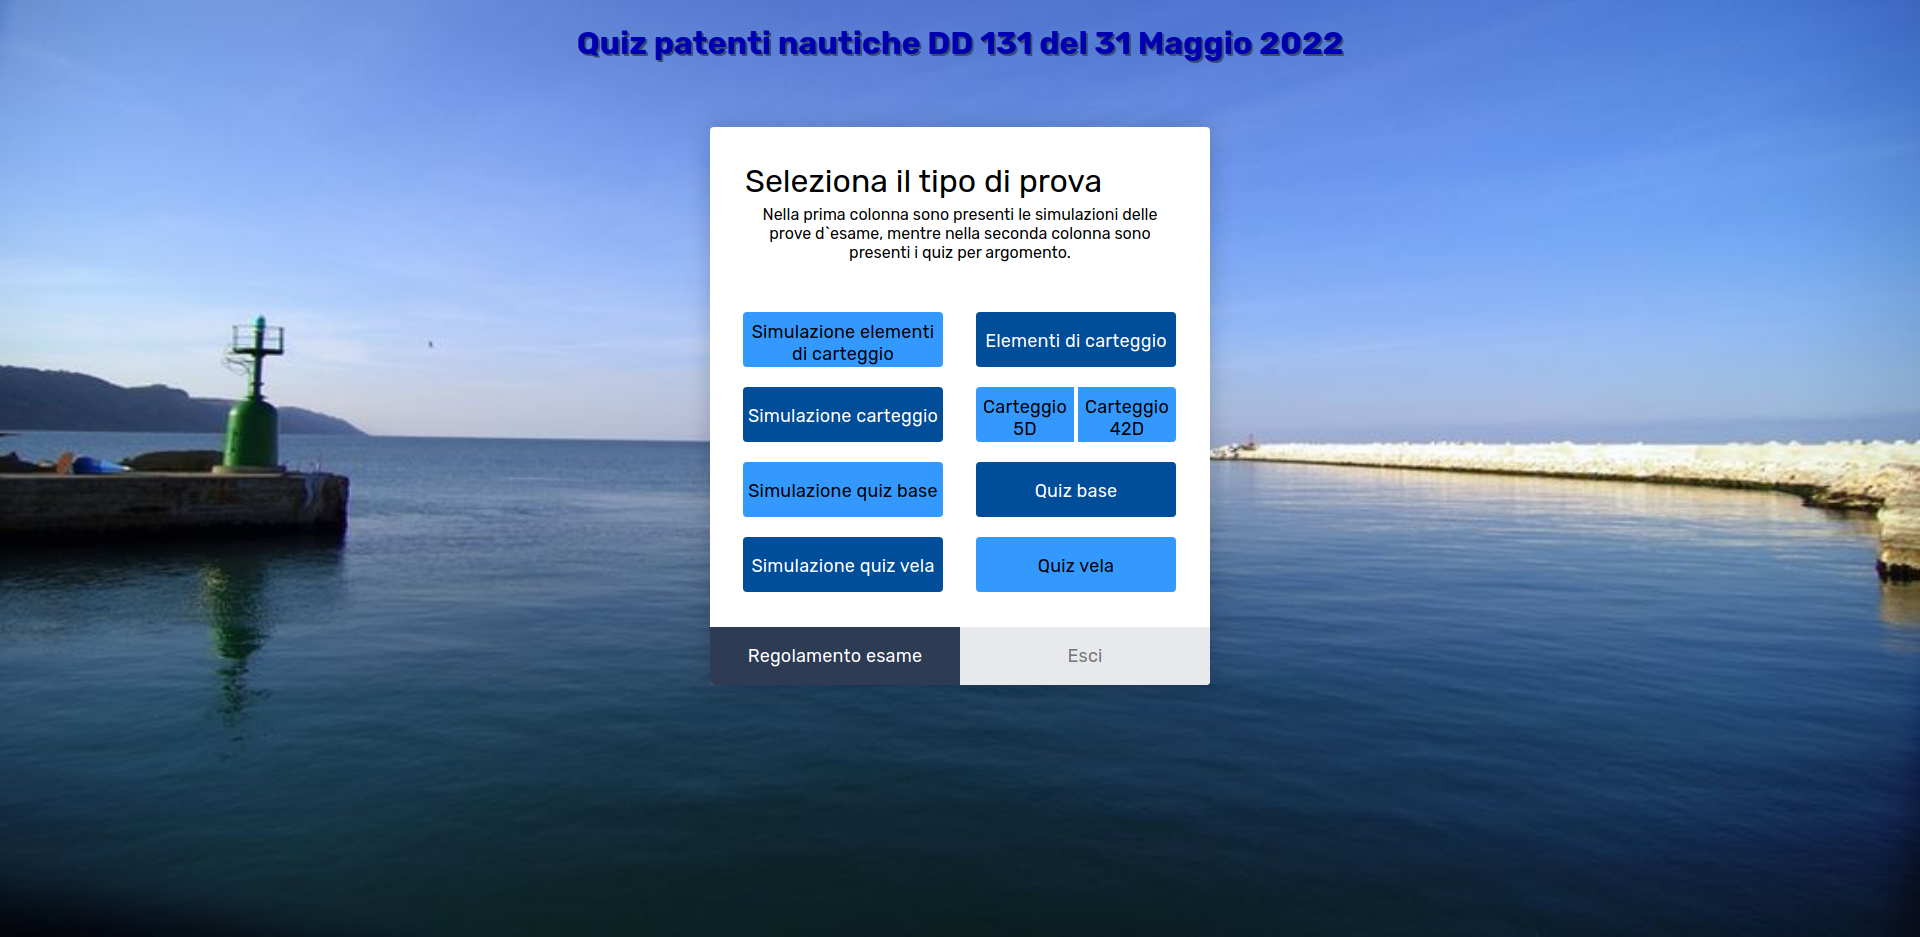
\includegraphics[scale=0.25]{Sites-images/07-Home_accesso_alle_prove.png}
		\caption{Pagina di selezione dei corsi.}
	\end{center}
\end{figure}

\textcolor{black}{Ora in ordine di rilevanza verranno presentati i file di ogni esercitazione, mettendo in evidenza le peculiarità di ognuno. I primi file saranno riportati maggiormente nella loro interezza in modo da esplicitare il metodo con il quale è stata condotta la costruzione dei restanti. Degli ultimi si riporteranno solo le parti salienti.}\\

\subsection{Presentazione delle pagine dei corsi}

\paragraph{\textcolor{black}{Simulazione elementi di carteggio}}\leavevmode\\
\raggedright
\begin{lstlisting}[language=php]
	if($_SESSION['permission'] !== "true"){
		/*control if user is logged*/
		if($_SESSION['mail'] !== null && $_SESSION['password'] !== null){
			
			$query = $utilities->getMysql()->query("SELECT password FROM user_table1 WHERE (email = '{$_SESSION['mail']}')");
			$tempArray = $query->fetch_array(MYSQLI_ASSOC);
			$password = $tempArray['password'];
			
			if($_SESSION['password'] !== $password){
				$_SESSION['user']     = "NotAllow";
				$_SESSION['mail']     = null;
				$_SESSION['password'] = null;
				header("Location: ../../main.php");
				exit;
			}
			/*in case of page reload*/
			$_SESSION['permission'] = "true";
			
		}else{
			$_SESSION['user']     = "NotAllow";
			$_SESSION['mail']     = null;
			$_SESSION['password'] = null;
			header("Location: ../../main.php");
			exit;
		}
	}
	
	/*find course properties*/
	$query = $utilities->getMysql()->query("SELECT * FROM charting_elements_properties WHERE (id = '1')");
	$tempArray = $query->fetch_array(MYSQLI_ASSOC);
	$maxQuestions = $tempArray['questions'];//<--- Very important field
	$maxErrors = $tempArray['errors'];//<--- Very important field
	
	/*find questions number*/
	$query = $utilities->getMysql()->query("SELECT COUNT(*) FROM charting_elements");
	$tempArray = $query->fetch_array(MYSQLI_ASSOC);
	$questionsNumber = $tempArray['COUNT(*)'];//<--- Very important field
	
	
	
	/*--------- GENERATE INDEXES AND EXTRACT QUESTIONS ----------*/
	
	$indexNumbers = array();
	$questions = array();
	
	$temp = 0;
	
	while($temp < $maxQuestions){
		
		if($_SESSION['numbers'][0] !== null){
			// if i'm here meaning that the page has been reloaded     
			if($indexNumbers[0] !== null){
				//generate number in recursive case
				$tempNum = random_int(1, $questionsNumber);
				//verify that the number isn't duplicated
				while(in_array($tempNum,$indexNumbers) || in_array($tempNum,$_SESSION['numbers'])){
					$tempNum = random_int(1, $questionsNumber);
				}
				
				//insert number
				$indexNumbers[$temp] = $tempNum; 
				
			}else{
				//generate number on base case
				$tempNum = random_int(1, $questionsNumber);
				//verify that the number is new (respect the past)
				while(in_array($tempNum,$_SESSION['numbers'])){
					$tempNum = random_int(1, $questionsNumber);
				}
				//insert number
				$indexNumbers[$temp] = $tempNum; 
			}
			
		}else{
			//if i'm here meaning that the page is new
			if($indexNumbers[0] !== null){
				//generate number in recursive case
				$tempNum = random_int(1, $questionsNumber);
				//verify that the number isn't duplicated
				while(in_array($tempNum,$indexNumbers)){
					$tempNum = random_int(1, $questionsNumber);
				}
				
				//insert number
				$indexNumbers[$temp] = $tempNum;
				
			}else{
				//generate number on base case
				$indexNumbers[$temp] = random_int(1, $questionsNumber);
			}
		}
		
		/*extract questions from db using the index generated*/
		$query = $utilities->getMysql()->query("SELECT * FROM charting_elements WHERE (id = '{$indexNumbers[$temp]}')");
		$tempArray = $query->fetch_array(MYSQLI_ASSOC);
		
		$questions[$temp] = array(
		"question_text"   => $tempArray['question_text'],
		"question1"       => $tempArray['question_1'],
		"question2"       => $tempArray['question_2'],
		"question3"       => $tempArray['question_3'],
		"question4"       => $tempArray['question_4'],
		"question5"       => $tempArray['question_5'],
		"answer1"         => $tempArray['answer_1'],
		"answer2"         => $tempArray['answer_2'],
		"answer3"         => $tempArray['answer_3'],
		"answer4"         => $tempArray['answer_4'],
		"answer5"         => $tempArray['answer_5'],
		);
		
		++$temp;
	}
	
	$_SESSION['numbers'] = $indexNumbers;
\end{lstlisting}

\textcolor{black}{Una delle prime operazioni che vengono svolte è il controllo dell'utente, per evitare l'accesso non autorizzato al servizio. Da notare inoltre che grazie alla variabile di sessione "permission" si garantisce che l'utente non venga espulso nel caso in cui ricarichi la pagina.\\
Successivamente si procede estraendo dal database le proprietà della simulazione, come il numero di domande da somministrare e il numero di errori massimi da poter commettere. Successivamente viene fatto il calcolo del numero delle domande presenti nel database in modo da poter stabilire il "range" per la selezione causale delle domande da presentare. Il fatto di contare ogni volta le domande presenti nel database garantisce che ogni nuova domanda inserita sia subito disponibile senza fare ulteriori aggiornamenti. Di conseguenza risulta semplificato il mantenimento e aggiornamento del database.\\
A questo punto si estraggono casualmente i vari indici delle domande da presentare. Questa operazione viene fatta con un ciclo "while" annidato che prosegue fino a che non siano stati generati senza ripetizioni (anche nei confronti dell'ultima esercitazione fatta) tutti gli indici richiesti. Per cercare di tenere alto il livello di efficienza delle operazioni l'ultima parte del ciclo "while" si compone della estrazione ed inserimento in un "array" delle domande permettendo di non dover svolgere un ulteriore ciclo.}\\
\bigskip
\textcolor{black}{Il codice "html" riportato inferiormente serve per mostrare come le informazioni estratte nella parte di "php" sono state integrate nella parte visibile della pagina. In generale si è usato il sistema "d'interrompere" il codice "html" richiamando il "tag" del "php" con l'ausilio comando "echo" per riportare le informazioni necessarie.}\\

\begin{lstlisting}[language=html]
	<!DOCTYPE html>
	<html lang="it" >
	<head>
	<meta charset="UTF-8">
	<title>Simulazione su elementi di carteggio nautico</title>
	<link rel='stylesheet' href='https://fonts.googleapis.com/css?family=Rubik:400,700'><link rel="stylesheet" href="simulationStyle.css">
	
	</head>
	<body>  
	
	<div class="welcomeText">
	<h1>Quiz patenti nautiche DD 131 del 31 Maggio 2022</h1>
	<h2>Simulazione sulle domande su elementi di carteggio nautico</h2>
	</div>
	
	<div class="question-form">
	<form method="post">
	<h1><?php
	if($indexNumbers[1] !== null){
		echo "Indice domande: ";
		$temp = 0;
		
		while($temp < $maxQuestions){
			echo $indexNumbers[$temp]." ";
			++$temp;
		}
		
	}else{
		echo "Indice domanda: ".$indexNumbers[0];
	}
	?>
	</h1>
	<div class="content">
	<?php 
	$temp = 0;
	while($temp < $maxQuestions){
		echo "<b>".$questions[$temp]["question_text"]."</b><br>";
		echo"<br>";
		echo $questions[$temp]["question1"]."<br>";
		echo $questions[$temp]["question2"]."<br>";
		echo $questions[$temp]["question3"]."<br>";
		echo $questions[$temp]["question4"]."<br>";
		echo $questions[$temp]["question5"]."<br>";
		echo"<br>";
		++$temp;
	}
	?> 
	</div>
	<div class="actions">
	<input type="button" name="revision" value="Guarda la soluzione" id="revision" onclick="check()"/>
	<div id="chart">Non hai la carta nautica? <a href="../Nautical_Charts/Carta_Nautica_5D.pdf" download> Scaricala qui</a></div>
	</div>
	<div id="answer">
	<?php
	$temp = 0;
	while($temp < $maxQuestions){
		if($indexNumbers[1] !== null){
			$tempNumber = $temp + 1;
			echo"<h3>Soluzione domanda: ".$tempNumber." </h3><br>"; 
		}
		echo"Soluzione quesito 1: <b>".$questions[$temp]["answer1"]."</b><br>";
		echo"Soluzione quesito 2: <b>".$questions[$temp]["answer2"]."</b><br>";
		echo"Soluzione quesito 3: <b>".$questions[$temp]["answer3"]."</b><br>";
		echo"Soluzione quesito 4: <b>".$questions[$temp]["answer4"]."</b><br>";
		echo"Soluzione quesito 5: <b>".$questions[$temp]["answer5"]."</b><br>";
		echo"<br>";
		++$temp;
	}
	?>
	<h3><?php
	if($maxErrors > 1){
		echo "La prova e' stata superata se si sono commessi massimo ".$maxErrors." errori.";
	}else{
		echo "La prova e' stata superata se e' stato commesso massimo ".$maxErrors." errore.";  
	}
	
	?></h3>
	</div>
	<div class="foot">
	<input type="submit" name="cancel" value="Esci dalla simulazione" id="button2"/>
	<input type="button" name="nextPage" value="Prova successiva" id="button1" onclick="next()"/>
	</div>
	</form>
	</div>
\end{lstlisting}

\textcolor{black}{Un problema che si solleva a questo punto dello sviluppo è la creazione di un sistema che permetta di nascondere la risposta del quesito, permettendo quindi l'esercizio. Questa cosa è realizzabile solo con il "javascript" che permette lato "front-end" di animare le varie parti del "html".\\
Si riportata lo "script" che è stato scritto per risolvere il problema.}\\

\begin{lstlisting}[language=java]
	<script>
	/*hide elements at the beginning*/
	var x = document.getElementById("answer");
	x.style.display = "none";
	/*show elements when the button is clicked*/
	function check(){
		var x = document.getElementById("answer");
		
		if(x.style.display === "none"){
			x.style.display = "block";
		}else{
			x.style.display = "none";
		}	
	}
	
	function next(){
		location.reload();  
	}
	</script>
\end{lstlisting}

\textcolor{black}{La funzione "check" viene evocata dal pulsante identificato come "revision" e permette di mostrare o di nascondere la parte in "html" contrassegnata come "answer" (inizialmente nascosta).\\
Siccome ogni esercitazione viene organizzata nella parte di codice in "php", eseguita soltanto durante il caricamento della pagina, come ultima cosa è stata dichiarata una funzione invocata dal pulsante "nextPage" per forzare il "reloading" della pagina, generando di fatto (nelle modalità vista prima) una nuova esercitazione.}\\
\vspace*{2mm}
\textcolor{black}{Finito di presentare il codice della simulazione, si desidera procedere con quello dell'esercitazione riferita sempre allo stesso tipo di domande. Incominciando ad analizzare il codice in "php"}.

%\vspace*{-0cm}

\begin{figure}[H]
	\begin{center}
		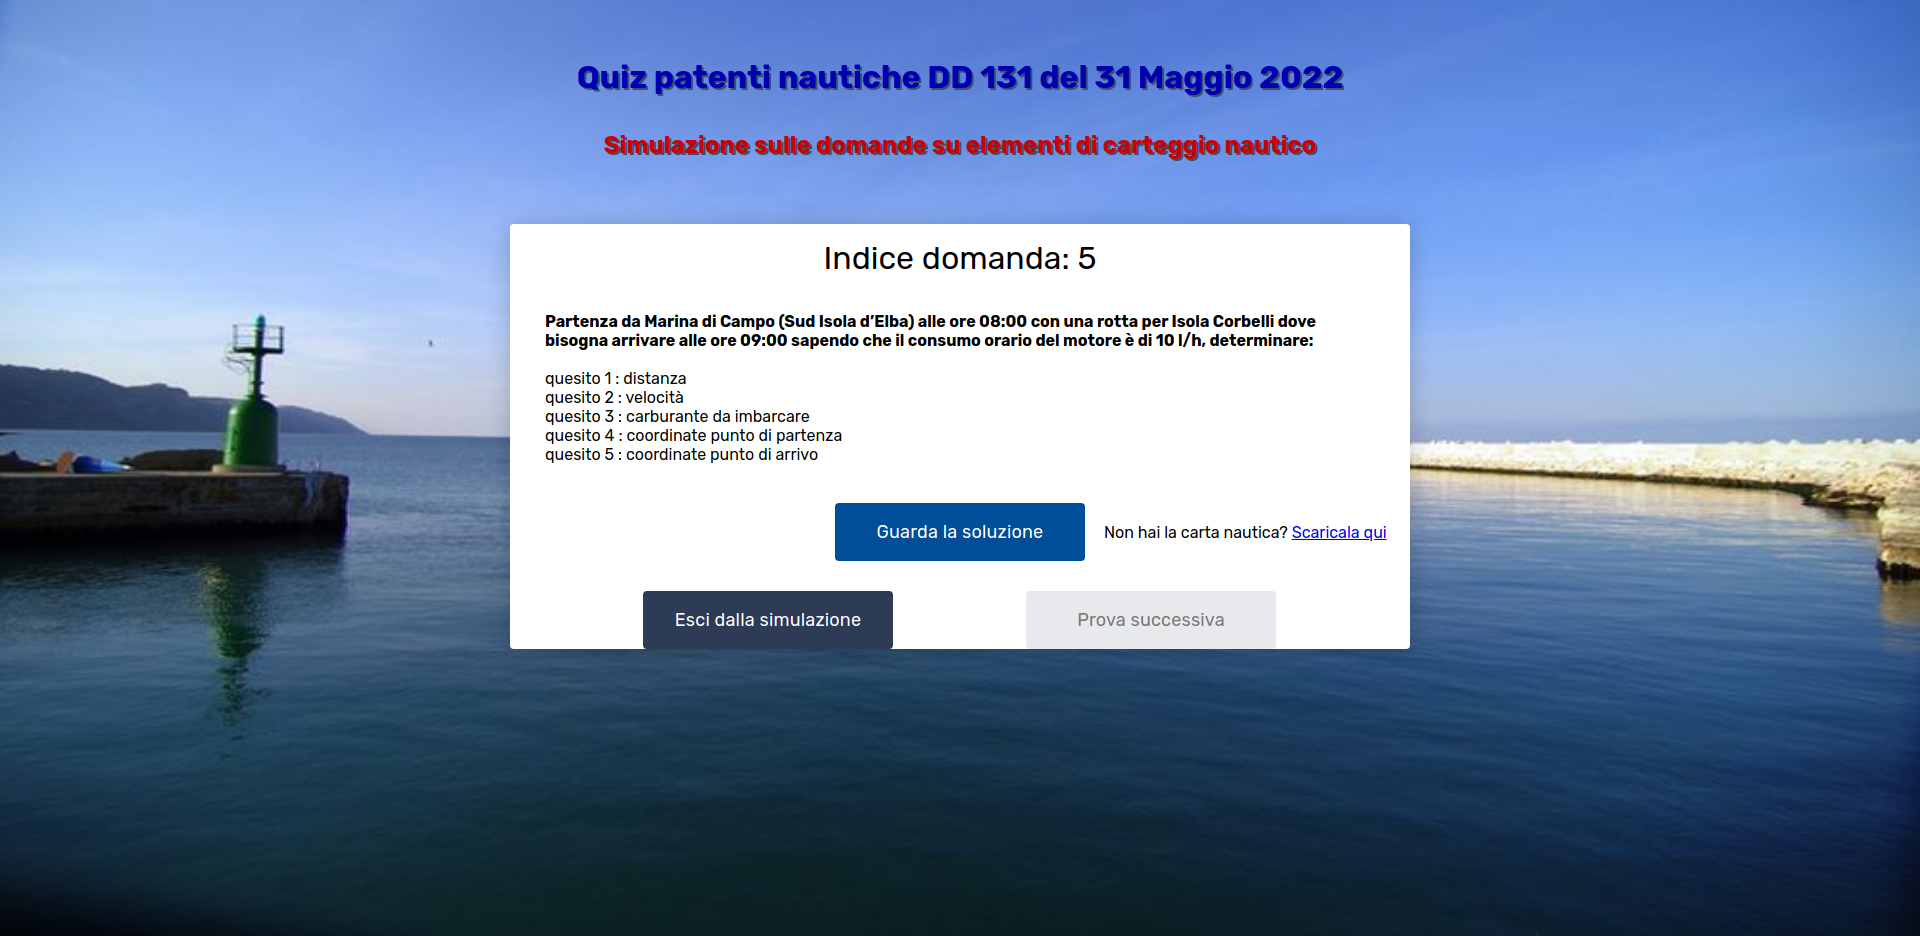
\includegraphics[scale=0.25]{Sites-images/12-Simulazione_elementi_di_carteggio.png}
		\caption{Pagina della simulazione elementi di carteggio.}
	\end{center}
\end{figure}
\vspace*{-1cm}
\begin{figure}[H]
	\begin{center}
		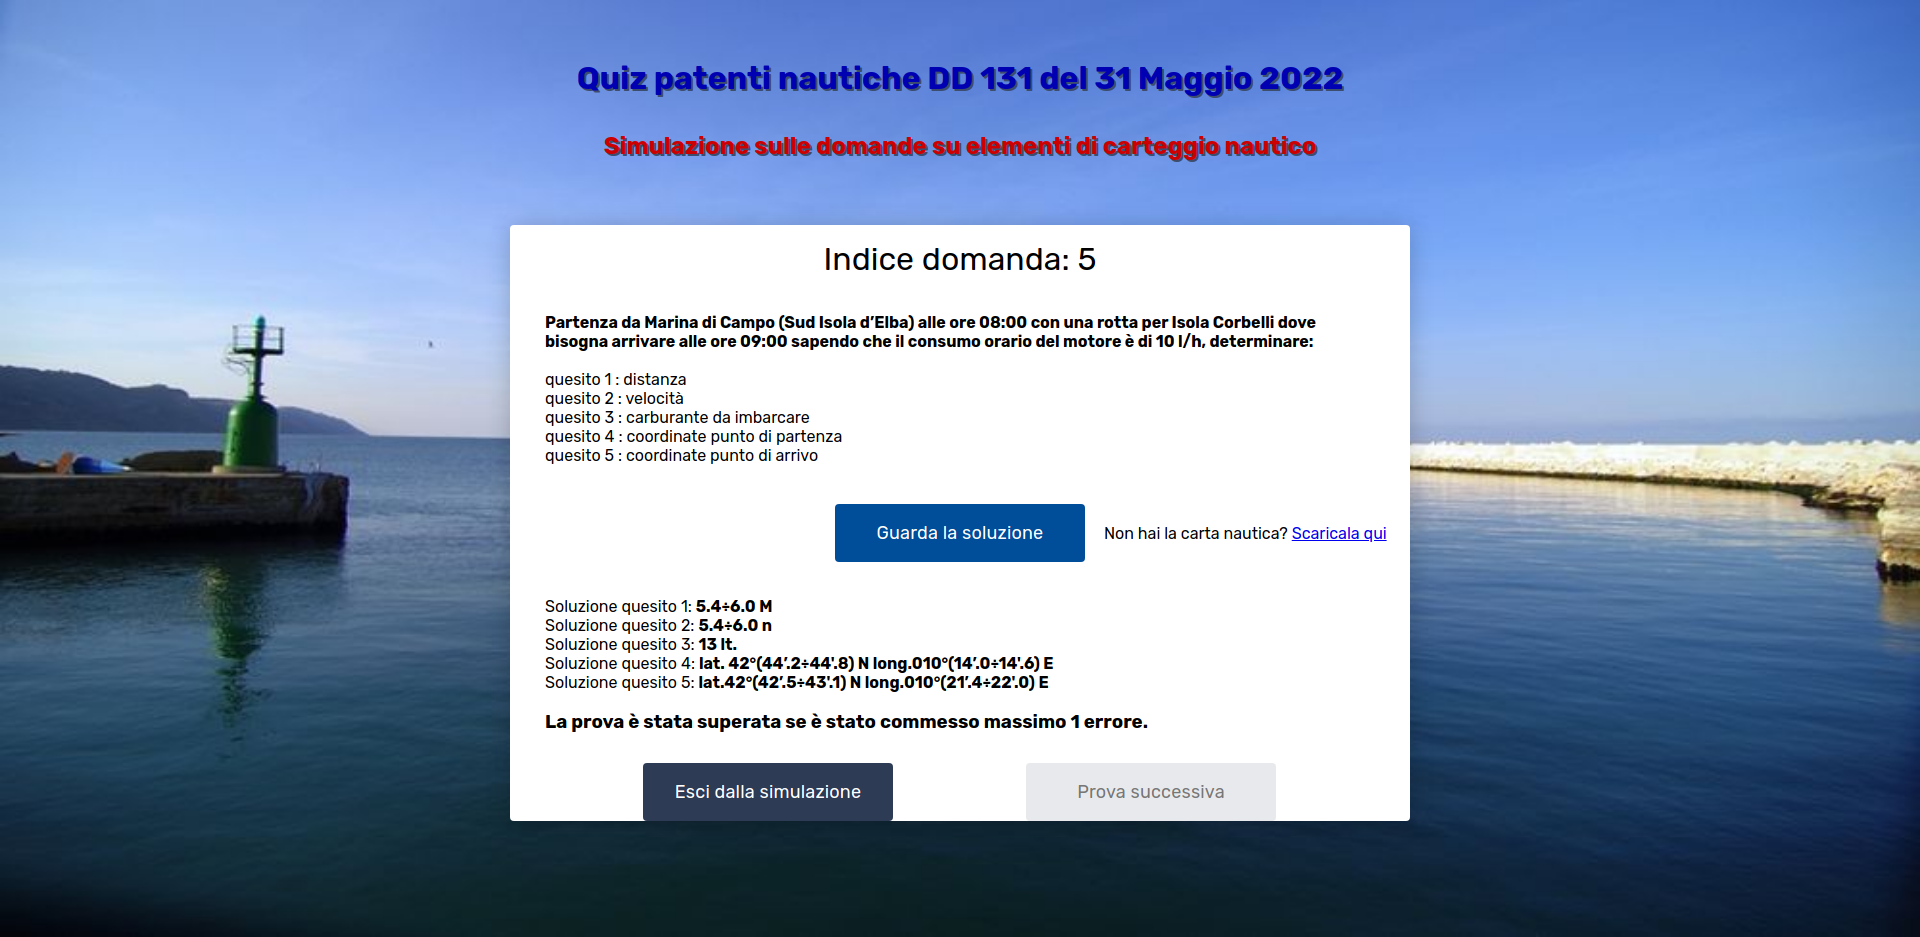
\includegraphics[scale=0.25]{Sites-images/13-Simulazione_elementi_di_carteggio-con_soluzioni.png}
		\caption{Pagina della simulazione elementi di carteggio con le soluzioni.}
	\end{center}
\end{figure}

\paragraph{\textcolor{black}{Elementi di carteggio (esercitazione)}}\leavevmode\\
\raggedright
\begin{lstlisting}[language=php]
	
	if($_SESSION['permission'] !== "true"){
		/*control if user is logged*/
		if($_SESSION['mail'] !== null && $_SESSION['password'] !== null){
			
			$query = $utilities->getMysql()->query("SELECT password FROM user_table1 WHERE (email = '{$_SESSION['mail']}')");
			$tempArray = $query->fetch_array(MYSQLI_ASSOC);
			$password = $tempArray['password'];
			
			if($_SESSION['password'] !== $password){
				$_SESSION['user']     = "NotAllow";
				$_SESSION['mail']     = null;
				$_SESSION['password'] = null;
				header("Location: ../../main.php");
				exit;
			}
			/*in case of page reload*/
			$_SESSION['permission'] = "true";
			
		}else{
			$_SESSION['user']     = "NotAllow";
			$_SESSION['mail']     = null;
			$_SESSION['password'] = null;
			header("Location: ../../main.php");
			exit;
		}
	}
	
	/*---------- END USER VERIFY ----------*/
	
	/*set count variable*/
	if($_SESSION['numbers'] == null){
		$_SESSION['numbers'] = 1;
	}
	
	
	/*find questions number*/
	$query = $utilities->getMysql()->query("SELECT COUNT(*) FROM charting_elements");
	$tempArray = $query->fetch_array(MYSQLI_ASSOC);
	$maxQuestions = $tempArray['COUNT(*)'];//<--- Very important field
	
	
	/*---------- START BUTTONS PART ----------*/
	
	if(isset($_POST['prevPage'])){
		if($_SESSION['numbers'] - 1 >= 1 && $_SESSION['numbers'] !== null){
			--$_SESSION['numbers'];
		}else{
			$utilities->Popup("Non e' possibile visualizzare la domanda precedente");
		}
	}
	
	if(isset($_POST['cancel'])){
		$_SESSION['permission'] = null;
		$_SESSION['numbers']     = null;
		header("Location: ../entry.php");
		exit;
	}
	
	if(isset($_POST['nextPage'])){
		if($_SESSION['numbers'] + 1 <= $maxQuestions && $_SESSION['numbers'] !== null){
			++$_SESSION['numbers'];
		}else{
			$utilities->Popup("Non e' possibile visualizzare la domanda successiva");
		}
	}
	
	/*---------- GENERATE QUESTIONS ----------*/
	
	$query = $utilities->getMysql()->query("SELECT * FROM charting_elements WHERE (id = '{$_SESSION['numbers']}')");
	$tempArray = $query->fetch_array(MYSQLI_ASSOC);
	$question_text = $tempArray['question_text'];
	$question1     = $tempArray['question_1'];
	$question2     = $tempArray['question_2'];
	$question3     = $tempArray['question_3'];
	$question4     = $tempArray['question_4'];
	$question5     = $tempArray['question_5'];
	$answer1       = $tempArray['answer_1'];
	$answer2       = $tempArray['answer_2'];
	$answer3       = $tempArray['answer_3'];
	$answer4       = $tempArray['answer_4'];
	$answer5       = $tempArray['answer_5'];
\end{lstlisting}

\textcolor{black}{Anche in questo caso la prima cosa che viene fatta è sempre il controllo dell'utente (da questo punto non più riportato nelle parti di codice successive).  Durante la generazione di una nuova esercitazione viene scritta una variabile di sessione con l'indice della domanda corrente, in modo che dopo il "reload" si possa accedere alla domanda successiva o alla precedente se è possibile (cioè a meno di non trovarsi agli estremi della lista di domande). Durante il primo accesso all'esercitazione la varaibile viene sempre instanziata con il valore di 1, siccome per specifica le domande sono conteggiate a partire dal numero 1 e non dallo 0 come abitudine informatica.\\
Saltata la parte che riguarda la gestione dei pulsantisi mostra come in questo caso, non dovendo gestire più di una domanda per volta,  si sia preferito dichiarare tante variabili quante le informazioni necessarie, al posto di dichiarare un "array" come nel caso precedente.\\
Lampante a questo punto sarà la semplicità con la quale le informazioni sono state riportate nella parte visibile della pagina. Dato che non è stato mostrato prima il codice "html" tipico delle esercitazioni, anche in questo caso viene riportato nella sua interezza, per dar modo di comprendere questo aspetto.}\\

\begin{lstlisting}[language=html]
	<html lang="it" >
	<head>
	<meta charset="UTF-8">
	<title>Esercitazione su elementi di carteggio nautico</title>
	<link rel='stylesheet' href='https://fonts.googleapis.com/css?family=Rubik:400,700'><link rel="stylesheet" href="exerciseStyle.css">
	
	</head>
	<body>  
	
	<div class="welcomeText">
	<h1>Quiz patenti nautiche DD 131 del 31 Maggio 2022</h1>
	<h2>Esercitazione sulle domande su elementi di carteggio nautico</h2>
	</div>
	
	<div class="question-form">
	<form method="post">
	<h1><?php
	echo "Indice domanda: ".$_SESSION['numbers']." / ". $maxQuestions;
	?>
	</h1>
	<div class="content">
	<?php 
	echo "<b>".$question_text."</b><br>";
	echo"<br>";
	echo $question1."<br>";
	echo $question2."<br>";
	echo $question3."<br>";
	echo $question4."<br>";
	echo $question5;
	?> 
	</div>
	<div class="actions">
	<input type="button" name="revision" value="Guarda la soluzione" id="revision" onclick="check()"/>
	<div id="chart">Non hai la carta nautica? <a href="../Nautical_Charts/Carta_Nautica_5D.pdf" download> Scaricala qui</a></div>
	</div>
	<div id="answer">
	<?php
	echo "Soluzione quesito 1: <b>".$answer1."</b><br>";
	echo "Soluzione quesito 2: <b>".$answer2."</b><br>";
	echo "Soluzione quesito 3: <b>".$answer3."</b><br>";
	echo "Soluzione quesito 4: <b>".$answer4."</b><br>";
	echo "Soluzione quesito 5: <b>".$answer5."</b>";
	?>
	</div>
	<div class="foot">
	<input type="submit" name="prevPage" value="Domanda precedente" id="button3"/>
	<input type="submit" name="cancel" value="Esci dalla esercitazione" id="button2"/>
	<input type="submit" name="nextPage" value="Domanda successiva" id="button1"/>
	</div>
	</form>
	</div>
\end{lstlisting}

\begin{minipage}{\textwidth}
%	\vspace*{-9cm}
	\raggedright
	\textcolor{black}{La parte di "scripting" non viene riportata poiché simile a quella precedente.}\\
\end{minipage}

\begin{minipage}{\textwidth}
	%\vspace*{-2cm}
	\begin{figure}[H]
		\begin{center}
			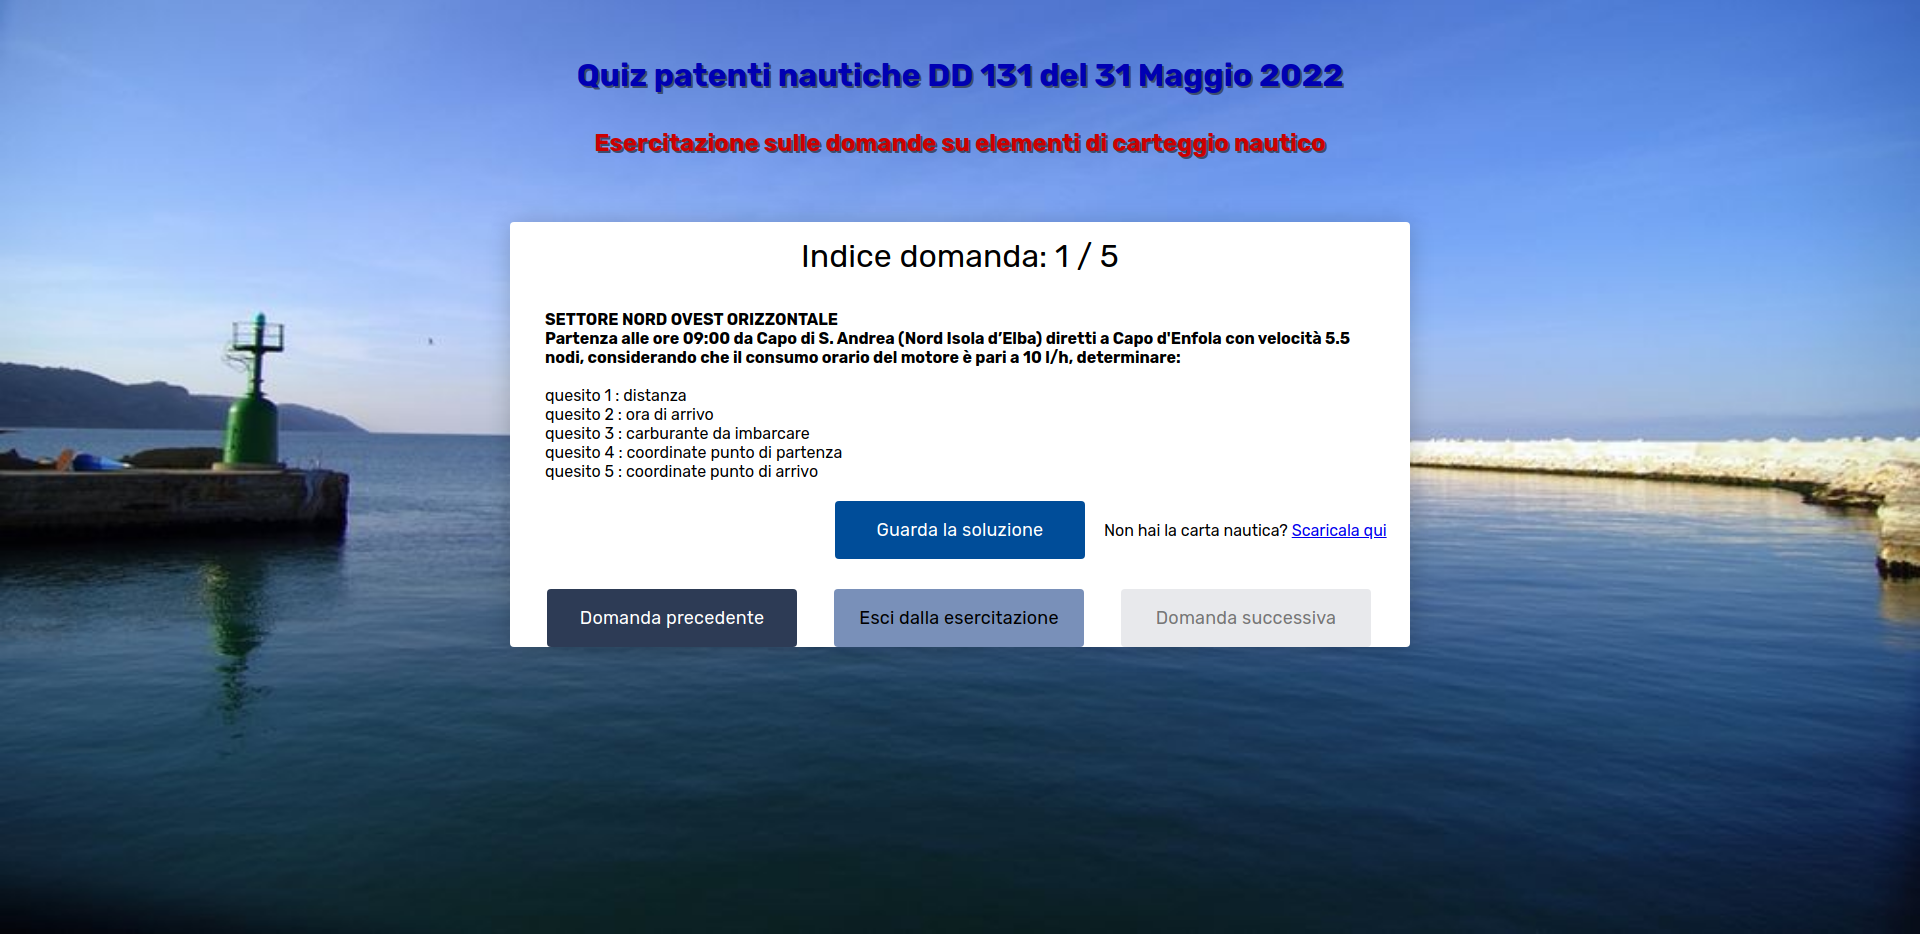
\includegraphics[scale=0.25]{Sites-images/14-Elementi_di_carteggio.png}
			\caption{Pagina degli elementi di carteggio.}
		\end{center}
	\end{figure}
\end{minipage}

\newpage

\begin{minipage}{\textwidth}
	\begin{figure}[H]
		\begin{center}
			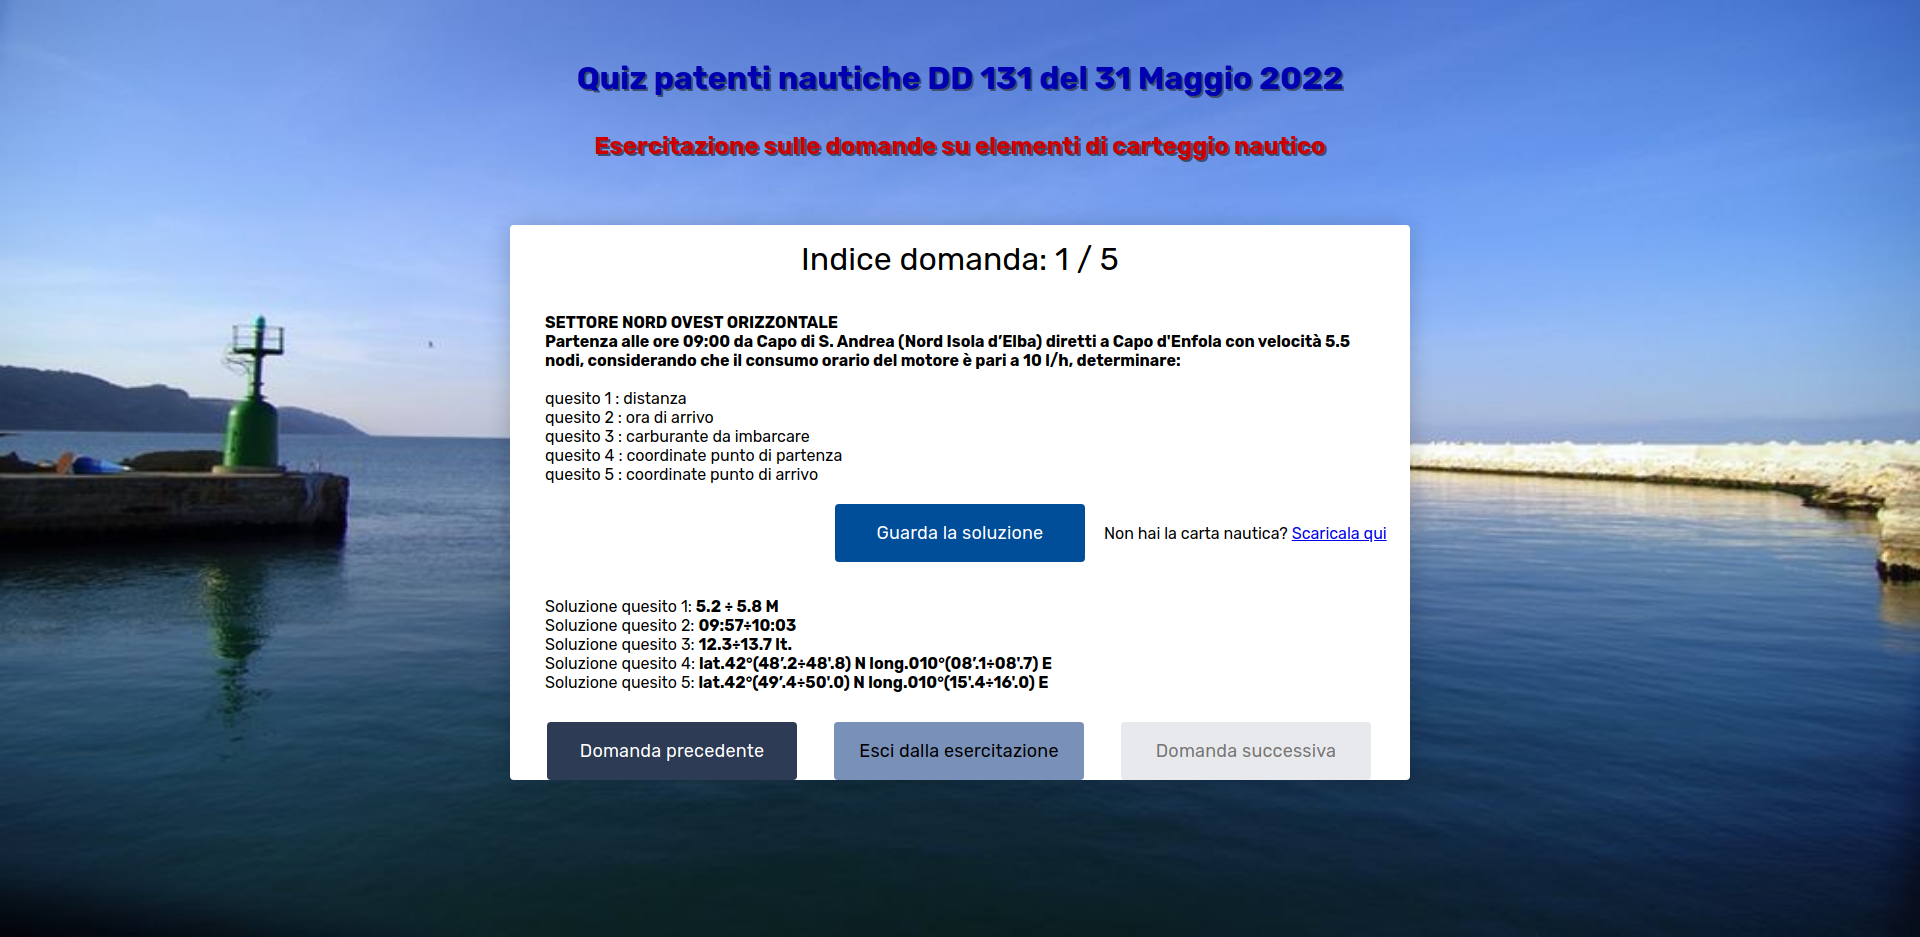
\includegraphics[scale=0.25]{Sites-images/15-Elementi_di_carteggio-con_soluzioni.png}
			\caption{Pagina degli elementi di carteggio con soluzioni.}
		\end{center}
	\end{figure}
\end{minipage}

\textcolor{black}{Si analizzano ora le peculiarità della prova di carteggio.}\\

\paragraph{\textcolor{black}{Simulazione carteggio}}\leavevmode\\
\raggedright
\textcolor{black}{La cosa che è d'interesse in questo caso è la gestione e presentazione di domande prese da due insiemi differenti, ovvero, quelle sulla carta nautica "5D" e "42D".}\\ 

\begin{lstlisting}[language=php]
	/*find course properties*/
	$query = $utilities->getMysql()->query("SELECT * FROM charting_test_properties WHERE (id = '1')");
	$tempArray = $query->fetch_array(MYSQLI_ASSOC);
	
	$max5DQuestions = $tempArray['5d_questions'];//<--- Very important field
	$max42DQuestions = $tempArray['42d_questions'];//<--- Very important field
	$maxErrors = $tempArray['errors'];//<--- Very important field
	
	/*find current questions numbers*/
	$query = $utilities->getMysql()->query("SELECT COUNT(*) FROM charting_test_5d");
	$tempArray = $query->fetch_array(MYSQLI_ASSOC);
	$questionsNumber5D = $tempArray['COUNT(*)'];//<--- Very important field
	
	$query = $utilities->getMysql()->query("SELECT COUNT(*) FROM charting_test_42d");
	$tempArray = $query->fetch_array(MYSQLI_ASSOC);
	$questionsNumber42D = $tempArray['COUNT(*)'];//<--- Very important field
	
	
	/*--------- GENERATE THE INDEXES AND extract questions---------*/
	$questionsIndex = 0;
	$indexNumbers = array();
	$questions = array();
	
	//---------- CHART 5D
	$temp = 0;
	while($temp < $max5DQuestions){
		
		if($_SESSION['numbers']['5d'][0] !== null){
			// if i'm here meaning that the page has been reloaded      
			if($indexNumbers['5d'][0] !== null){
				//generate number in recursive case
				$tempNum = random_int(1, $questionsNumber5D); // this 1 is because i know that the questions starts form 1 into db
				//verify that number isn't duplicated
				while(in_array($tempNum,$indexNumbers['5d']) || in_array($tempNum,$_SESSION['numbers']['5d'])){
					$tempNum = random_int(1, $questionsNumber5D);
				}
				
				//insert number
				$indexNumbers['5d'][$temp] = $tempNum; 
				
			}else{
				//generate number on base case
				$tempNum = random_int(1, $questionsNumber5D);
				//verify that the number is new (respect the past)
				while(in_array($tempNum,$_SESSION['numbers']['5d'])){
					$tempNum = random_int(1, $questionsNumber5D);
				}
				//insert number
				$indexNumbers['5d'][$temp] = $tempNum; 
			}
			
		}else{
			
			//if i'm here meaning that the page is new
			if($indexNumbers['5d'][0] !== null){
				//generate number in recursive case
				$tempNum = random_int(1, $questionsNumber5D);
				//verify that the number isn't duplicated
				while(in_array($tempNum,$indexNumbers['5d'])){
					$tempNum = random_int(1, $questionsNumber5D);
				}
				
				//insert number
				$indexNumbers['5d'][$temp] = $tempNum;
				
			}else{
				//generate number on base case
				$indexNumbers['5d'][$temp] = random_int(1, $questionsNumber5D);
			}
		}
		
		//extract questions from db
		$query = $utilities->getMysql()->query("SELECT * FROM charting_test_5d WHERE (id = '{$indexNumbers['5d'][$temp]}')");
		$tempArray = $query->fetch_array(MYSQLI_ASSOC);  
		
		$questions[$questionsIndex] = array(
		"index"         => $tempArray['id'],
		"question_text" => $tempArray['question_text'],
		"answer"        => $tempArray['answer'],
		"area"		=> $tempArray['area'],
		"is42d"         => false,
		);
		++$questionsIndex;
		
		++$temp;
	}
	
	//---------- CHART 42D
	$temp = 0;
	while($temp < $max42DQuestions){
		
		if($_SESSION['numbers']['42d'][0] !== null){
			// if i'm here meaning that the page has been reloaded     
			if($indexNumbers['42d'][0] !== null){
				//generate number in recursive case
				$tempNum = random_int(1, $questionsNumber42D); // this 1 is because i know that the questions starts form 1 into db
				//verify that the number isn't duplicated
				while(in_array($tempNum,$indexNumbers['42d']) || in_array($tempNum,$_SESSION['numbers']['42d'])){
					$tempNum = random_int(1, $questionsNumber42D);
				}
				
				//insert number
				$indexNumbers['42d'][$temp] = $tempNum; 
				
			}else{
				//generate number on base case
				$tempNum = random_int(1, $questionsNumber42D);
				//verify that the number is new (respect the past)
				while(in_array($tempNum,$_SESSION['numbers']['42d'])){
					$tempNum = random_int(1, $questionsNumber42D);
				}
				//insert number
				$indexNumbers['42d'][$temp] = $tempNum; 
			}
			
		}else{
			//if i'm here meaning that the page is new
			if($indexNumbers['42d'][0] !== null){
				//generate number in recursive case
				$tempNum = random_int(1, $questionsNumber42D);
				//verify that the number isn't duplicated
				while(in_array($tempNum,$indexNumbers['42d'])){
					$tempNum = random_int(1, $questionsNumber42D);
				}
				
				//insert number
				$indexNumbers['42d'][$temp] = $tempNum;
				
			}else{
				//generate number on base case
				$indexNumbers['42d'][$temp] = random_int(1, $questionsNumber42D);
			}
		}
		
		//extract questions from db
		$query = $utilities->getMysql()->query("SELECT * FROM charting_test_42d WHERE (id = '{$indexNumbers['42d'][$temp]}')");
		$tempArray = $query->fetch_array(MYSQLI_ASSOC);  
		
		$questions[$questionsIndex] = array(
		"index"         => $tempArray['id'],
		"question_text" => $tempArray['question_text'],
		"answer"        => $tempArray['answer'],
		"area"		=> $tempArray['area'],	
		"is42d"         => true,
		);
		++$questionsIndex;
		
		++$temp;
	}
	
	
	$_SESSION['numbers'] = $indexNumbers;
	
	$totalQuestions = count($questions);
\end{lstlisting}\leavevmode\newline

\begin{minipage}{\textwidth}
	\vspace*{-32cm}
	
	\textcolor{black}{In generale l'estrazione delle domande non avviene in modi differenti rispetto a quanto presentato in passato. Si può osservare che per ogni tipo di domande è stato fatto un ciclo "while" con la stessa logica del precedente. In questo caso la scelta di un doppio ciclo (uno per ogni insieme di domande) potrebbe non risultare tra le più efficienti in assoluto, ma aumenta la semplicità del codice, permettendo di vedere il problema del reperimento delle informazioni come diviso in due parti. Però si è comunque cercato di rendere il codice efficiente usando un solo "array" (al posto di due come si sarebbe portati a pensare) per memorizzare tutte le domande estratte, in modo da risparmiare spazio in memoria. Il campo "is42d" permette di distinguere tra i due tipi di domande.\\
	Il resto del codice della pagina non presenta ulteriori diversità.
	}\\
\end{minipage}%\leavevmode\newpage

%\restoregeometry

\begin{minipage}{\textwidth}
	\begin{figure}[H]
		\begin{center}
			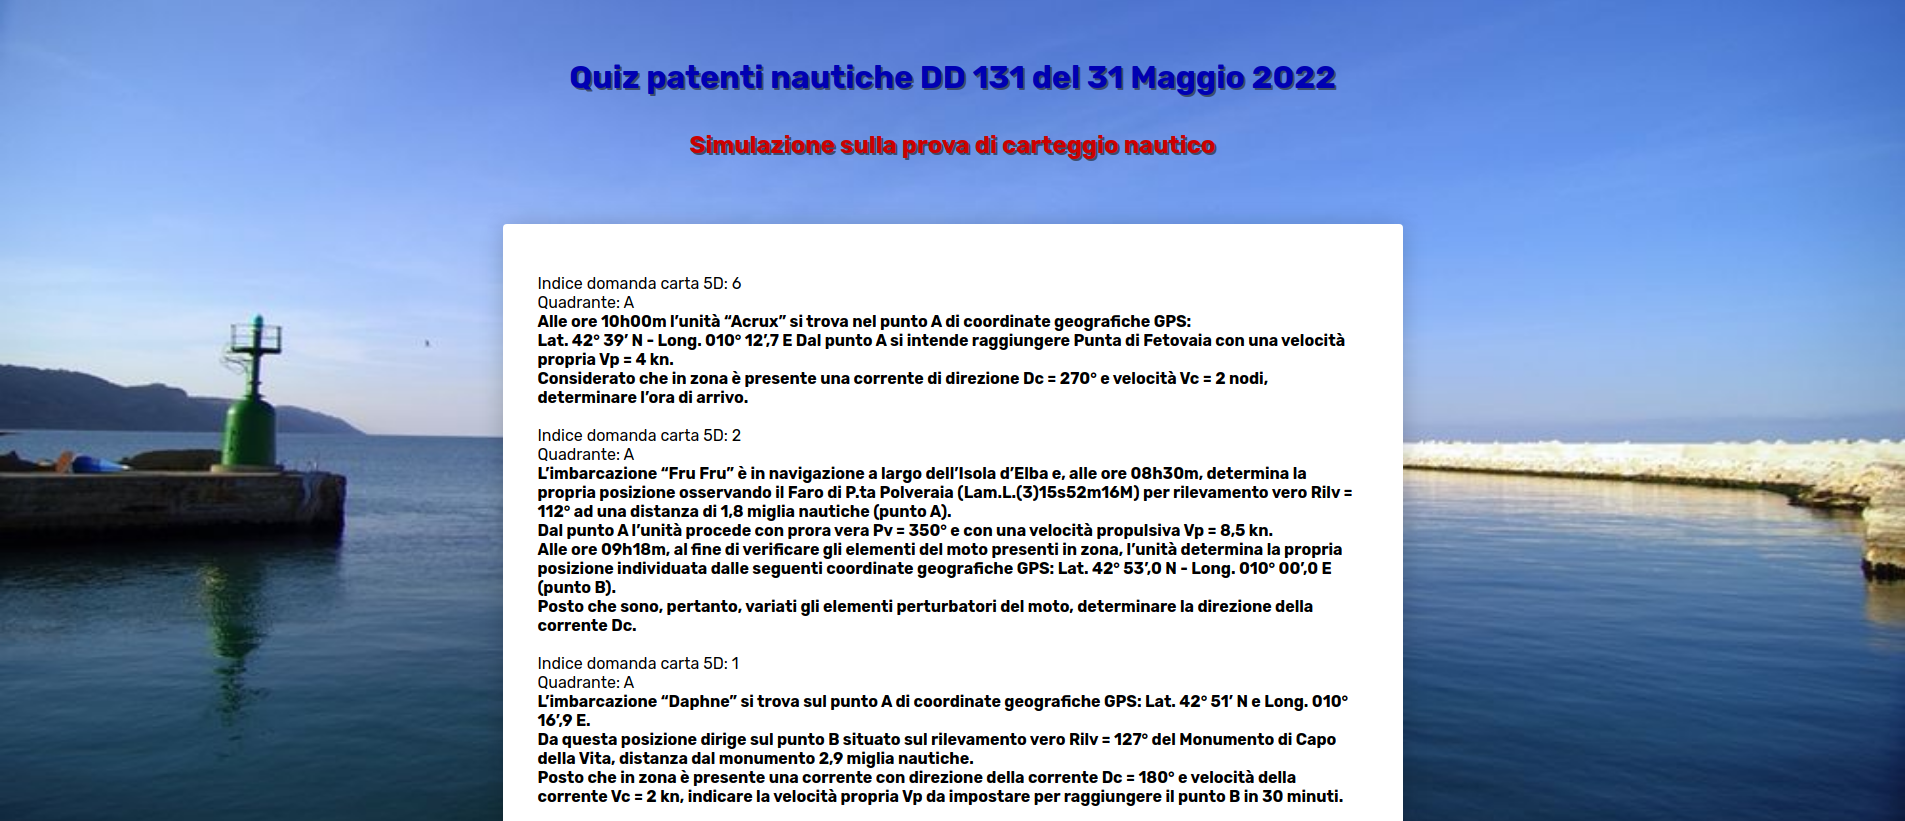
\includegraphics[scale=0.25]{Sites-images/16-Simulazione_carteggio1.png}
			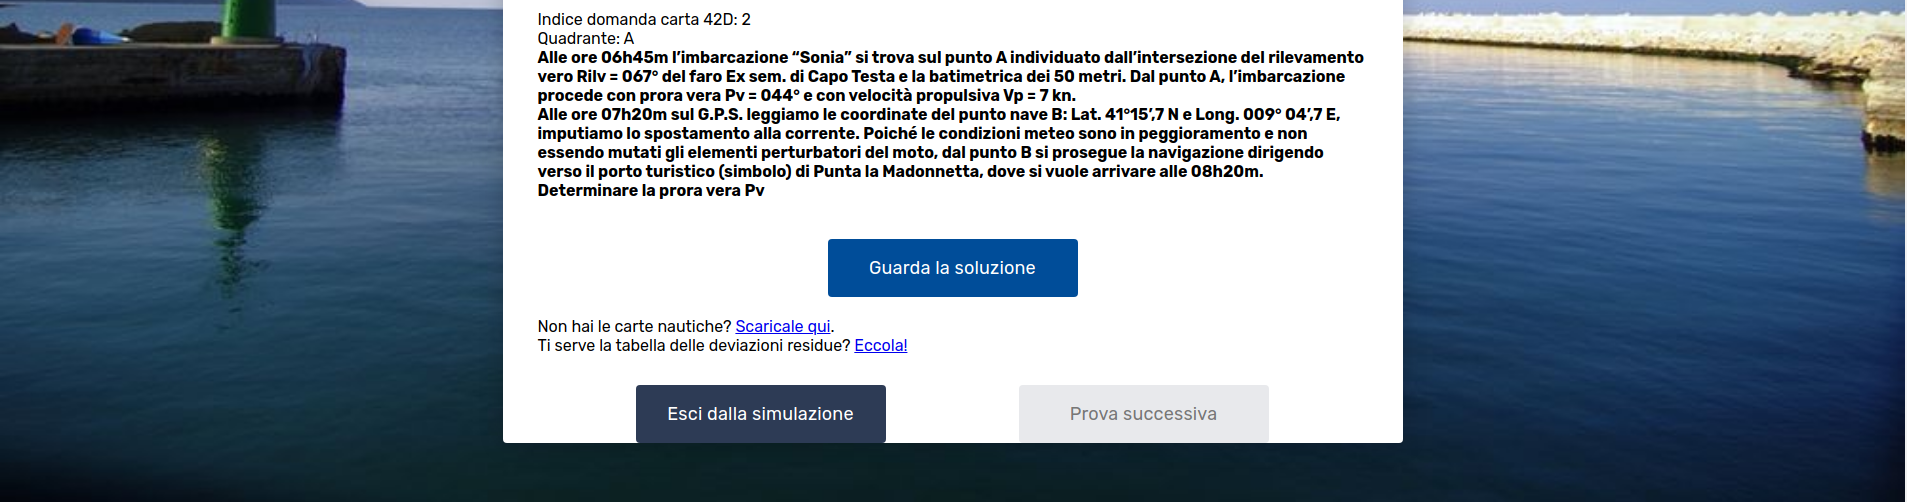
\includegraphics[scale=0.25]{Sites-images/17-Simulazione_carteggio2.png}
			\caption{Pagina di simulazione del carteggio.}
			(Ricomposta)
		\end{center}
	\end{figure}
	
	\begin{figure}[H]
		\begin{center}
			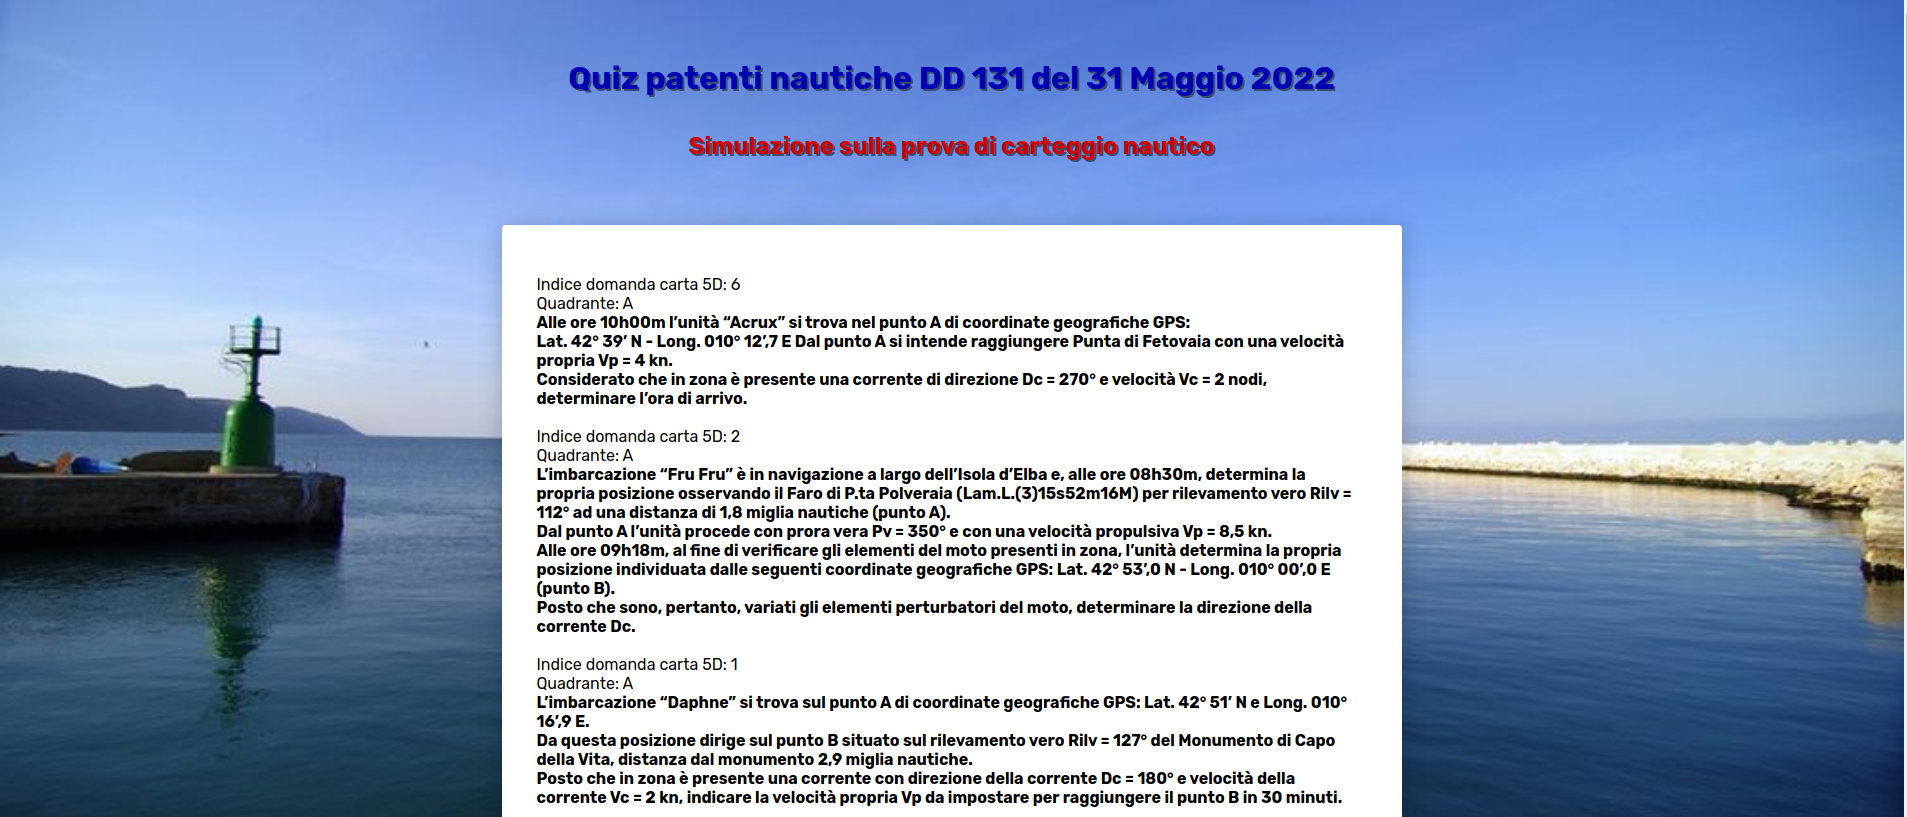
\includegraphics[scale=0.25]{Sites-images/18-Simulazione_carteggio-con_soluzioni1.png}
			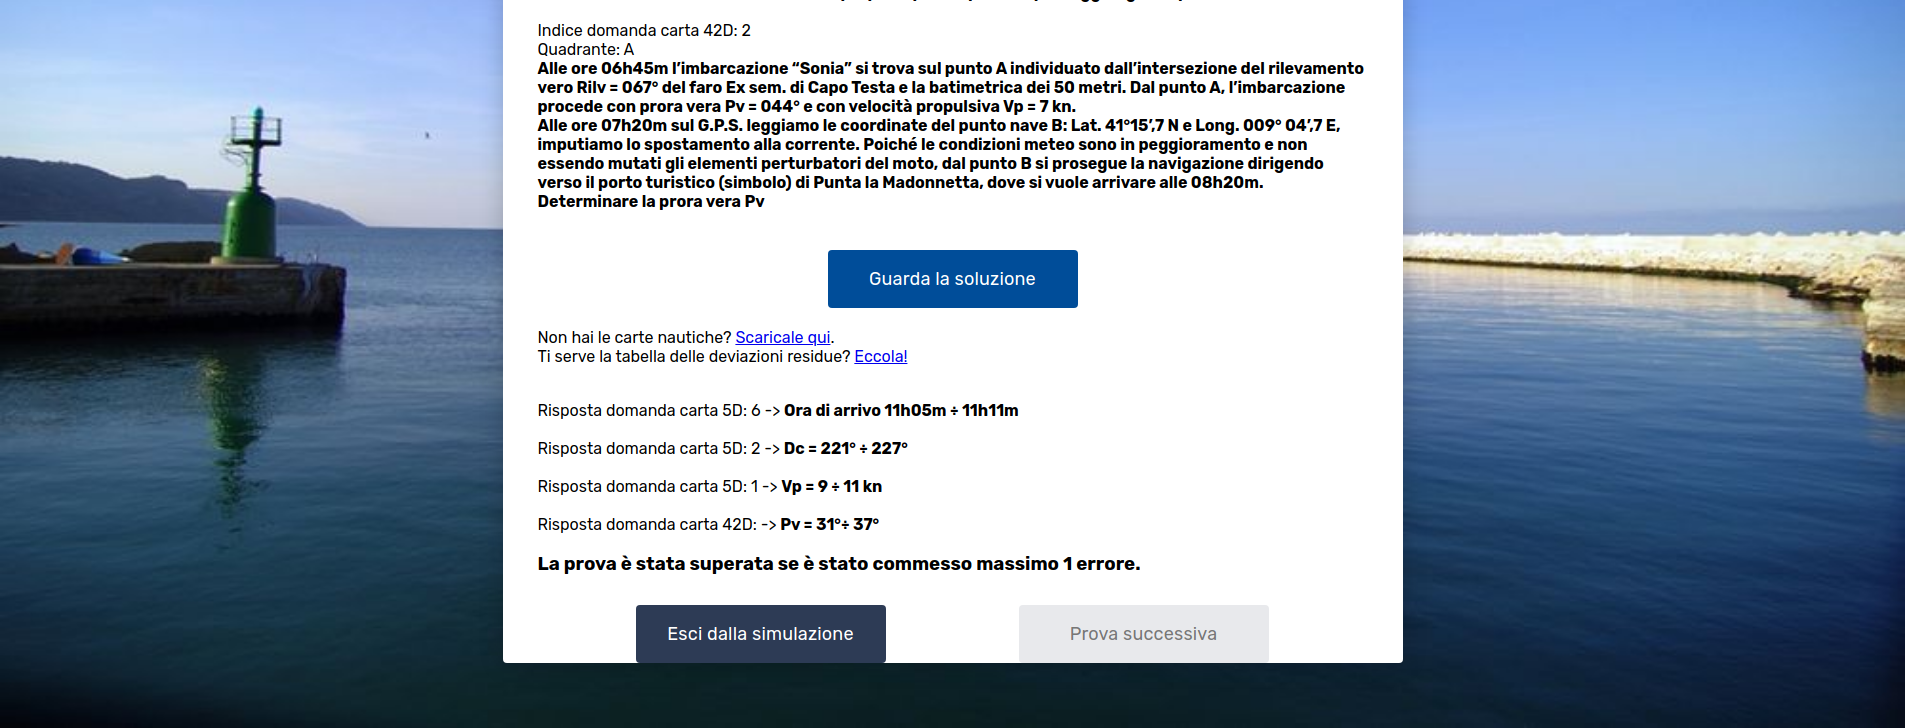
\includegraphics[scale=0.25]{Sites-images/19-Simulazione_carteggio-con_soluzioni2.png}
			\caption{Pagina di simulazione del carteggio con soluzioni.}
			(Ricomposta)
		\end{center}
	\end{figure}
\end{minipage}

\paragraph{\textcolor{black}{Carteggio 5D e 42D (esercitazione)}}\leavevmode\\
\textcolor{black}{Durante la spiegazione di questa parte, sono state accorpate le due pagine distinte per l'esercitazione nelle due categorie di domande, siccome risultano identiche tranne per il tipo di domande puntate.\\
Le domande presenti in questa sezione sono divisibili per argomenti, motivo per cui all'inizio della esercitazione viene chiesto di quale argomento caricare le domande. Questo tipo di gestione comporta che la parte di codice in "php" debba collaborale con quella in "javascrpit" in modo tale che tramite quest'ultima l'utente possa selezionare l'argomento tra quelli presenti nel database e che la parte in "php" possa dunque caricare le domande richieste. Il passaggio delle informazioni tra il "front-end" ed il "back-end" è fatto attraverso l'impostazione di argomenti nel "url", siccome ci sono dei problemi con il funzionamento di "AJAX". Questo aspetto sarà affrontato più avanti con la presentazione di un caso nel quale l'uso di "AJAX" sarebbe stato particolarmente conveniente.\\
Il codice per la gestione delle domande è riportato inferiormente.}\newline 

\textbf{\textcolor{black}{Parte di codice php}}\\

\begin{lstlisting}[language=php]
/*---------- RETRIEVE URL TOPIC ----------*/
$Array = $urlUtility->getInfoFromUrl($_SERVER['REQUEST_URI']);

if($Array['topic'] !== null && $Array['topic'] !== $_SESSION['topic']){
	$_SESSION['topic'] = $Array['topic'];
	
	/*change temp array to determinate questions*/
	$query = $utilities->getMysql()->query("SELECT * FROM charting_test_5d WHERE (topic = '{$Array['topic']}')");
	$tempArray = $query->fetch_all(MYSQLI_ASSOC);
	$_SESSION['maxQuestions'] = null;
	$_SESSION['questions']    = $tempArray;
	$_SESSION['numbers']       = 0;
}

/*--------- QUESTIONS PREPARATION ----------*/

$id       = null;
$topic    = null;
$question = null;
$answer   = null;
if($_SESSION['maxQuestions'] == null){
	$_SESSION['maxQuestions'] = count($_SESSION['questions']);
}

/*extract questions*/
if($_SESSION['questions'] !== null && $_SESSION['numbers'] !== null){
	
	$id = $_SESSION['questions'][$_SESSION['numbers']]['id'];
	$topic = $_SESSION['questions'][$_SESSION['numbers']]['topic'];
	$question = $_SESSION['questions'][$_SESSION['numbers']]['question_text'];
	$answer = $_SESSION['questions'][$_SESSION['numbers']]['answer'];
	$area = $_SESSION['questions'][$_SESSION['numbers']]['area'];	
}
\end{lstlisting}

\vspace*{1.5cm}

\textcolor{black}{\textbf{Parte di codice html}. \\Per mostrare com'è fatto il menu a tendina poi utilizzato con il "javascrpit".}\\

\begin{lstlisting}[language=html]
	 <input type="button" onclick="dropFunction()" class="dropbtn" name="dropdown" value="Seleziona capitolo">
	
	<div id="myDropdown" class="dropdown-content">
	<?php
	$query = $utilities->getMysql()->query("SELECT DISTINCT topic FROM charting_test_5d");
	$tempArray = $query->fetch_all(MYSQLI_ASSOC);
	foreach($tempArray as $arr1){
		foreach($arr1 as $arr2){
			$var = "'".$arr2."'";
			echo '<a onclick="setArgument('.$var.')">'.$arr2.'</a>';
		}
	}		
	
	?>			
\end{lstlisting}

\textcolor{black}{\textbf{Parte di codice javascript}}\\

\begin{lstlisting}[language=java]
	<script type='text/javascript'>
	
	//hide revision elements at the beginning
	var x = document.getElementById("answer");
	x.style.display = "none";
	
	//show elements when the revision button is clicked
	function check(){
		var x = document.getElementById("answer");
		
		if(x.style.display === "none"){
			x.style.display = "block";
		}else{
			x.style.display = "none";
		}	
	}
	
	//dropdown button toggle to hide and show contents
	function dropFunction() {
		document.getElementById("myDropdown").classList.toggle("show");
	}
	
	// close dropdown menu when is clicked outside of it
	window.onclick = function(event) {
		if (!event.target.matches('.dropbtn')) {
			var dropdowns = document.getElementsByClassName("dropdown-content");
			var i;
			for (i = 0; i < dropdowns.length; i++) {
				var openDropdown = dropdowns[i];
				if (openDropdown.classList.contains('show')) {
					openDropdown.classList.remove('show');
				}
			}
		}
	}
	
	// set the argument topic to url
	function setArgument(topic){
		var URL = window.location.href;
		var data ={'topic': topic};
		var parameters = new URLSearchParams(data);
		window.location.href = URL.split('?')[0]+"?"+parameters;
	}
	</script>
\end{lstlisting}

\begin{minipage}{\textwidth}
%	\vspace*{-25cm}
	
	\textcolor{black}{Nel codice riportato si può vedere come il menu a tendina definito nella parte "html" e gestito con il "javascript" permetta all'utente di selezionare l'argomento. Quest'ultimo poi viene passato alla parte in "php" tramite impostazione "dell'url" fatto con l'ultima funzione definita in "javascript".\\
	La gestione delle domande caricate in base all'argomento è deducibile in quanto molto simile a casi precedenti.}\\
\end{minipage}%\leavevmode\newpage

%\vspace*{-15cm}
\begin{minipage}{\textwidth}
	\begin{center}
		\textbf{Esempio delle pagine del carteggio sulla carta 5d.}
	\end{center}
	
	\begin{figure}[H]
		\begin{center}
			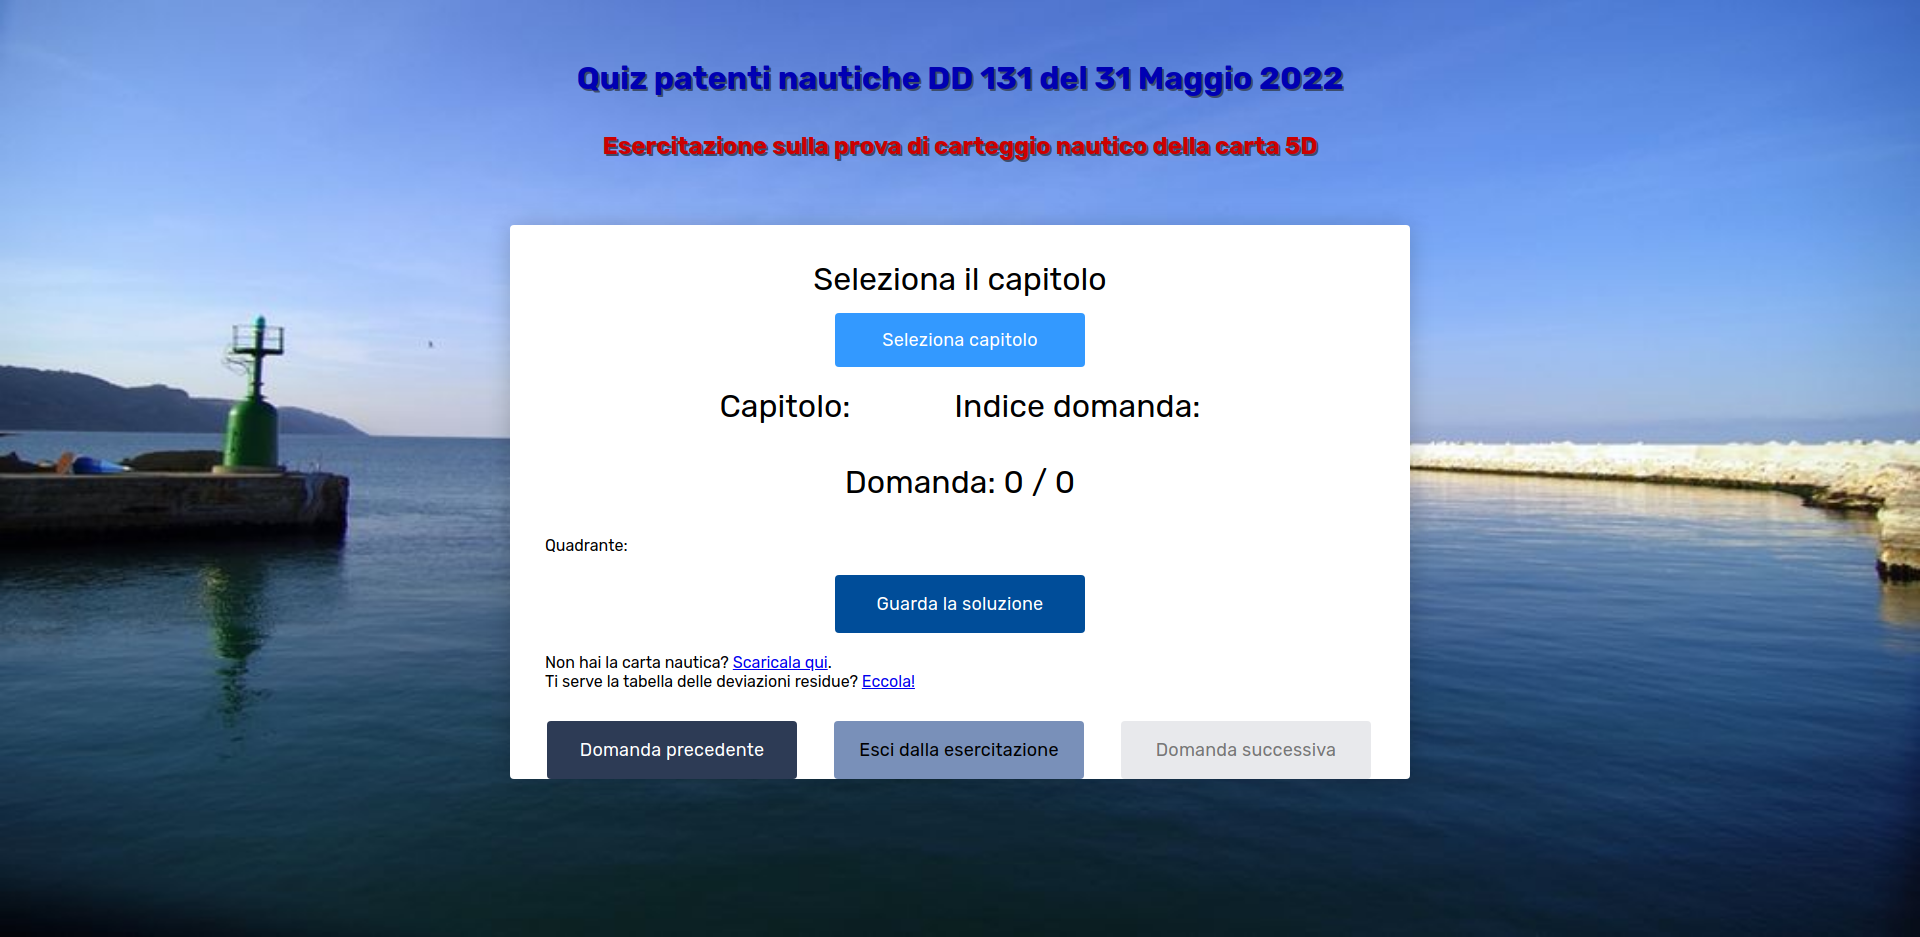
\includegraphics[scale=0.25]{Sites-images/20-Carteggio_5d.png}
			\caption{Pagina di carteggio sulla carta 5d.}
		\end{center}
	\end{figure}
	\end{minipage}
	\newpage
	
	\begin{minipage}{\textwidth}
	\begin{figure}[H]
		\begin{center}
			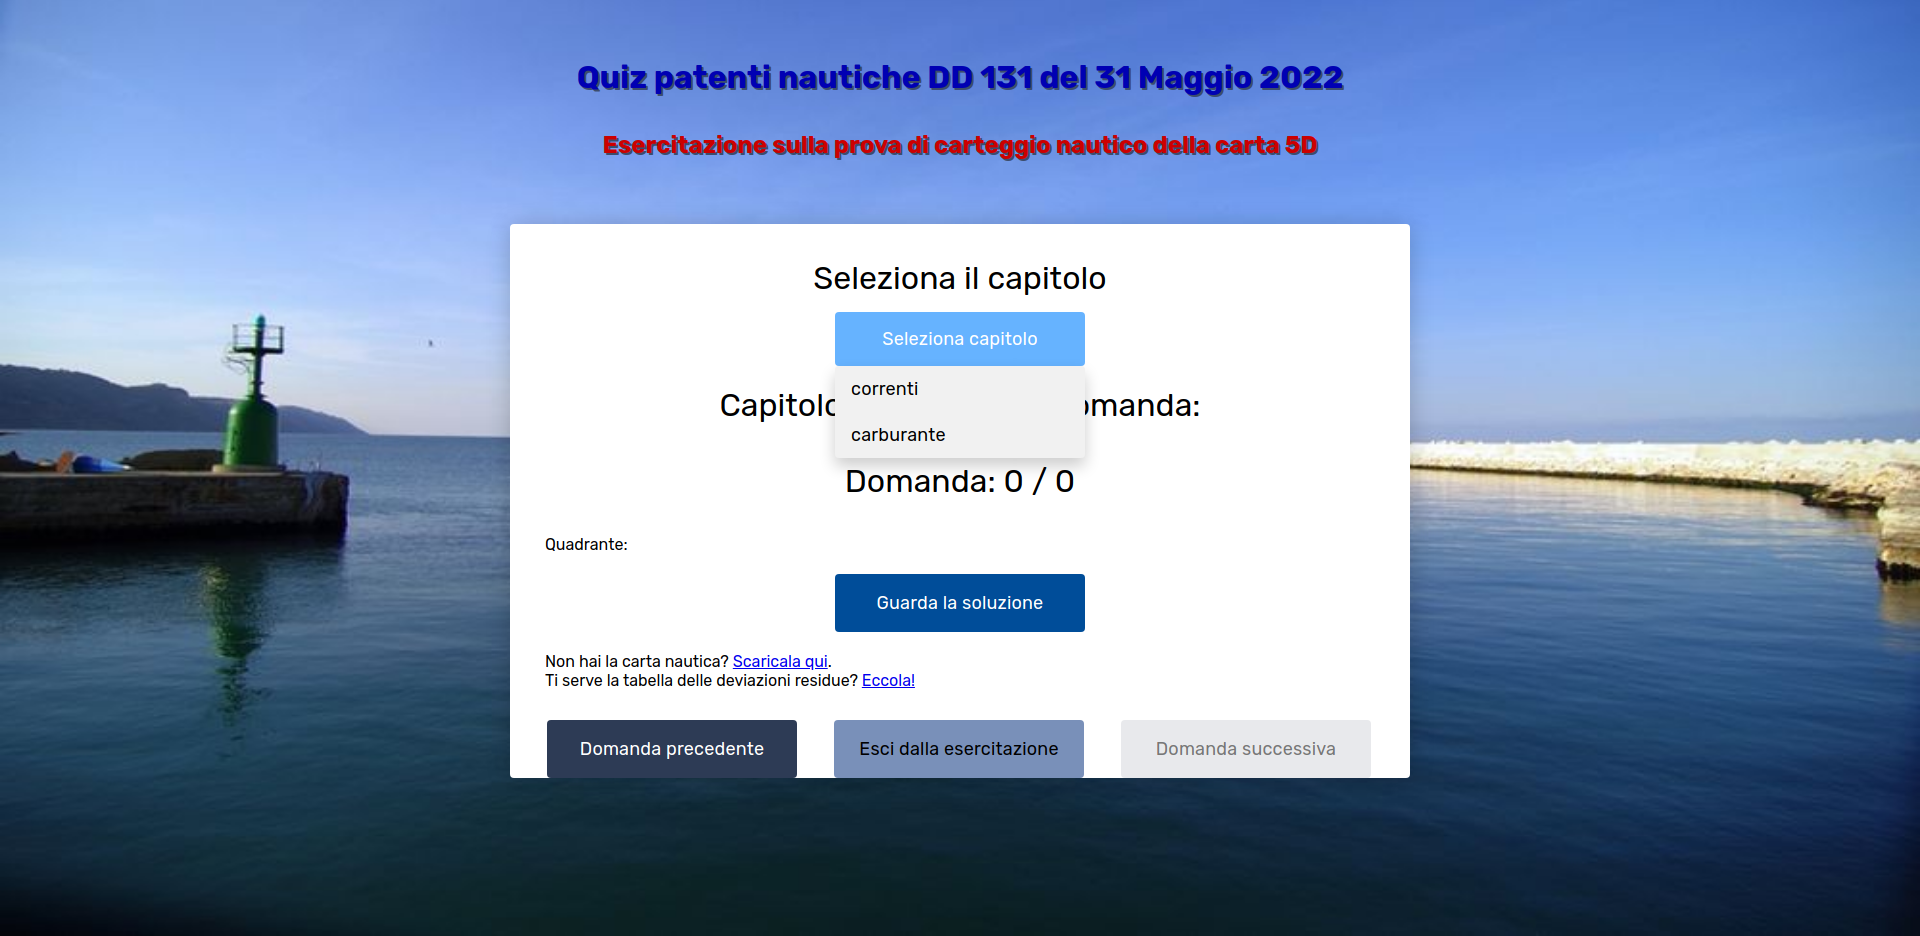
\includegraphics[scale=0.25]{Sites-images/21-Carteggio_5d_Selezione.png}
			\caption{Pagina di carteggio sulla carta 5d con selezione.}
		\end{center}
	\end{figure}

\begin{figure}[H]
	\begin{center}
		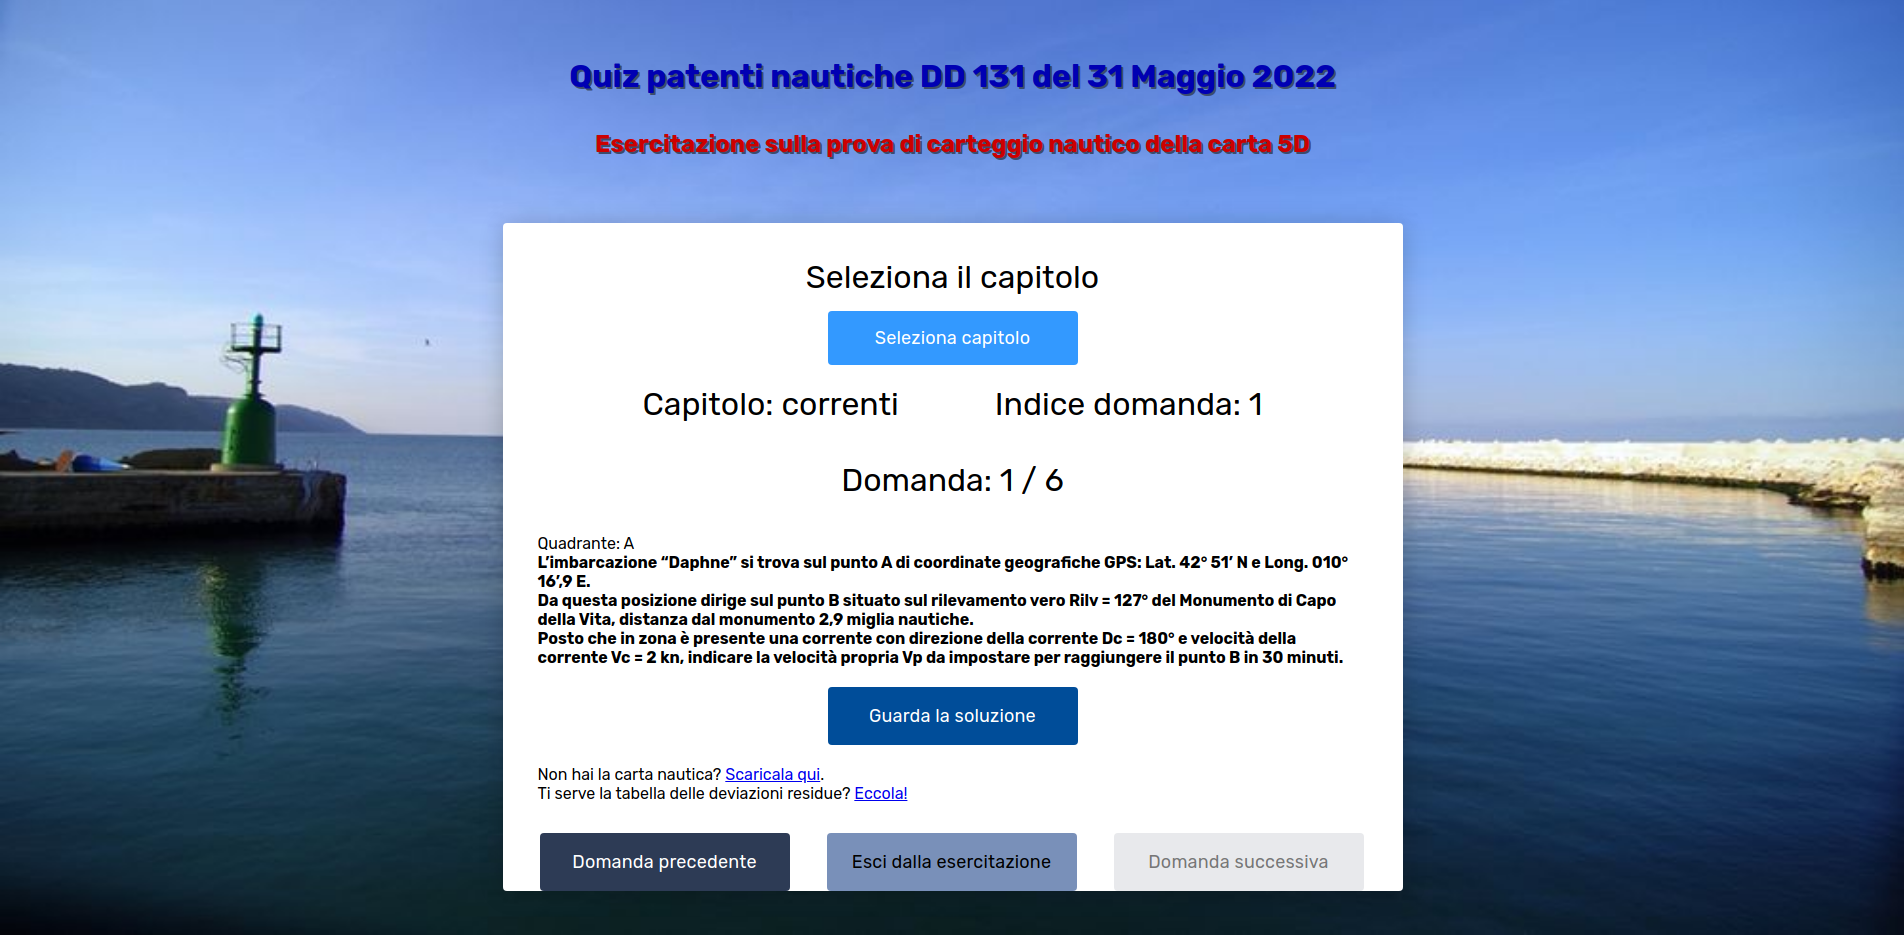
\includegraphics[scale=0.25]{Sites-images/22-Carteggio_5d_Domanda.png}
		\caption{Pagina di carteggio sulla carta 5d con la domanda.}
	\end{center}
\end{figure}

\begin{figure}[H]
	\begin{center}
		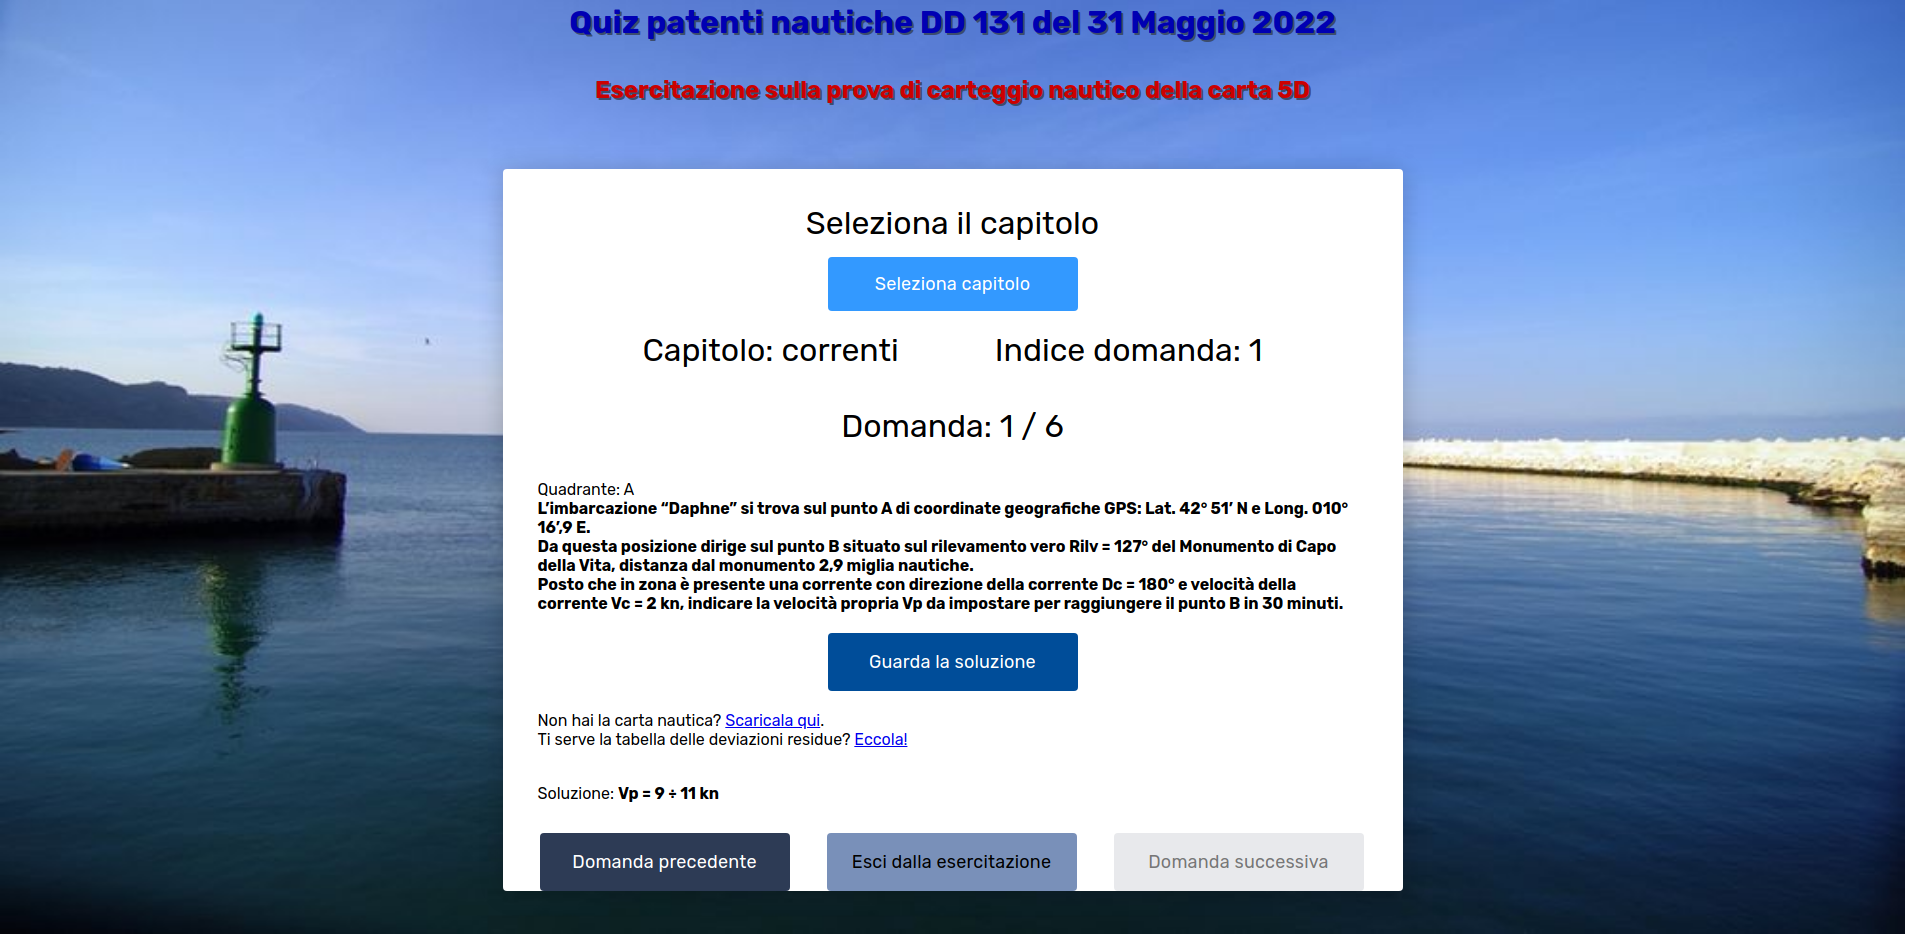
\includegraphics[scale=0.25]{Sites-images/23-Carteggio_5d_Risposta.png}
		\caption{Pagina di carteggio sulla carta 5d con la risposta.}
	\end{center}
\end{figure}
\end{minipage}


\textcolor{black}{Ora si passa alla presentazione delle parti salienti del codice della simulazione ed esercitazione per i quiz di base.}\\

\paragraph{\textcolor{black}{Simulazione quiz base}}\leavevmode\\
\raggedright
\textcolor{black}{Il codice che amministra questa simulazione è più complesso rispetto ai precedenti, per questa prova bisogna selezionare (in base al regolamento) una certa quantità di domande per ogni argomento ma per semplificare il database, le domande sono state inserite tutte nella stessa tabella e sono distinguibili attraverso l'argomento di appartenenza e dall'indice assoluto stabilito dal regolamento. Questa soluzione permette una manutenzione facilitata in caso di aggiornamento delle domande.\\
Però rende il codice più complesso, dovendo in primo luogo estrarre per ogni argomento il "range" tra gli indicici in cui fare la selezione causale delle domande.\\
Per questo motivo non verrà riportato tutto il codice, ma solo quello che mostra l'intera gestione delle domande di un singolo argomento, in modo da poter semplificare la lettura e la comprensione.}\\

\begin{lstlisting}[language=php]
	/*---------- EXTRACT QUESTIONS PROPERTIES ----------*/
	$query = $utilities->getMysql()->query("SELECT * FROM base_quiz_properties WHERE (id = '1')");
	$tempArray = $query->fetch_array(MYSQLI_ASSOC);
	
	$teoria_dello_scafo_questions                      = $tempArray['teoria_dello_scafo_questions'];
	$motori_questions                                  = $tempArray['motori_questions'];
	$sicurezza_della_navigazione_questions             = $tempArray['sicurezza_della_navigazione_questions'];
	$manovra_e_condotta_questions                      = $tempArray['manovra_e_condotta_questions'];
	$colreg_e_segnalamento_marittimo_questions         = $tempArray['colreg_e_segnalamento_marittimo_questions'];
	$meteorologia_questions                            = $tempArray['meteorologia_questions'];
	$navigazione_cartografica_ed_elettronica_questions = $tempArray['navigazione_cartografica_ed_elettronica_questions'];
	$normativa_diportistica_e_ambientale_questions     = $tempArray['normativa_diportistica_e_ambientale_questions'];
	$errors                                            = $tempArray['errors'];
	
	/*---------- FIND RANGE TO GENERATE QUESTIONS ----------*/
	$teoria_dello_scafo_questions_range = array();
	
	//---------- TEORIA DELLO SCAFO
	$query = $utilities->getMysql()->query("SELECT MIN(DISTINCT id) AS id FROM base_quiz WHERE (topic = 'TEORIA DELLO SCAFO')");
	$tempArray = $query->fetch_array(MYSQLI_ASSOC);
	$teoria_dello_scafo_questions_range['min'] = $tempArray['id'];
	$query = $utilities->getMysql()->query("SELECT MAX(DISTINCT id) AS id FROM base_quiz WHERE (topic = 'TEORIA DELLO SCAFO')");
	$tempArray = $query->fetch_array(MYSQLI_ASSOC);
	$teoria_dello_scafo_questions_range['max'] = $tempArray['id'];
	
	/*--------- PART TO GENERATE THE INDEXES AND TO CATCH THE QUESTIONS---------*/
	
	// variables where save indexes
	$indexNumbers = array();
	$questions = array();
	$indexQuestions = 0; //this will be increased after every question inserted.
	
	/---------- TEORIA DELLO SCAFO
	//-> $teoria_dello_scafo_questions
	//-> $teoria_dello_scafo_questions_range
	//-> teoria_dello_scafo
	$temp = 0;
	while($temp < $teoria_dello_scafo_questions){
		
		if($_SESSION['numbers']['teoria_dello_scafo'] !== null){
			// if i'm here meaning that the page has been reloaded
			if($indexNumbers['teoria_dello_scafo'][0] !== null){
				//generate number in recursive case
				$tempNum = random_int($teoria_dello_scafo_questions_range['min'], $teoria_dello_scafo_questions_range['max']);
				//verify that the number isn't duplicated
				while(in_array($tempNum,$indexNumbers['teoria_dello_scafo']) || in_array($tempNum,$_SESSION['numbers']['teoria_dello_scafo'])){
					$tempNum = random_int($teoria_dello_scafo_questions_range['min'], $teoria_dello_scafo_questions_range['max']);
				}
				
				//insert number
				$indexNumbers['teoria_dello_scafo'][$temp] = $tempNum;
				
			}else{
				//generate number on base case
				$tempNum = random_int($teoria_dello_scafo_questions_range['min'], $teoria_dello_scafo_questions_range['max']);
				//verify that the number is new (respect the past)
				while(in_array($tempNum,$_SESSION['numbers']['teoria_dello_scafo'])){
					$tempNum = random_int($teoria_dello_scafo_questions_range['min'], $teoria_dello_scafo_questions_range['max']);
				}
				//insert number
				$indexNumbers['teoria_dello_scafo'][$temp] = $tempNum;
			}
			
		}else{
			//if i'm here meaning that the page is new
			if($indexNumbers['teoria_dello_scafo'][0] !== null){
				//generate number in recursive case
				$tempNum = random_int($teoria_dello_scafo_questions_range['min'], $teoria_dello_scafo_questions_range['max']);
				//verify that the number isn't duplicated
				while(in_array($tempNum,$indexNumbers['teoria_dello_scafo'])){
					$tempNum = random_int($teoria_dello_scafo_questions_range['min'], $teoria_dello_scafo_questions_range['max']);
				}
				
				//insert number
				$indexNumbers['teoria_dello_scafo'][$temp] = $tempNum;
				
			}else{
				//generate number on base case
				$indexNumbers['teoria_dello_scafo'][$temp] = random_int($teoria_dello_scafo_questions_range['min'], $teoria_dello_scafo_questions_range['max']);
			}
		}
		/*catch question*/
		$query = $utilities->getMysql()->query("SELECT * FROM base_quiz WHERE (id = '{$indexNumbers['teoria_dello_scafo'][$temp]}')");
		$tempArray = $query->fetch_array(MYSQLI_ASSOC);
		$questions[$indexQuestions] = $tempArray;
		++$indexQuestions;
		
		++$temp;
		}
		
		$_SESSION['numbers'] = $indexNumbers;
		
		// get current number of loaded questions
		$totalQuestions = count($questions);
		
		/*--------- PREPARE ARRAY WITH ANSWER FOR CHECKING PART IN JS---------*/
		$questionsAnswers = array();
		
		$temp = 0;
		while($temp < $totalQuestions){
			
			$questionsAnswers[$temp]['answer_1'] = $questions[$temp]['answer_1'];
			$questionsAnswers[$temp]['answer_2'] = $questions[$temp]['answer_2'];
			$questionsAnswers[$temp]['answer_3'] = $questions[$temp]['answer_3'];
			
			++$temp;
		}
\end{lstlisting}
\textcolor{black}{Si può notare che la logica di fondo non è stata stravolta ma è stata adeguata al specifico caso, infatti, come anche in precedenza, le domande sono state tutte inserite in un "array" comune e l'inserimento è stato fatto come di consueto alla fine dei cicli "while" annidati per poter risparmiare risorse. La novità principale in questo caso risiede nel sistema un pochino più complesso di selezione delle domande.\\
Rispetto al passato dove la risposta alle domande era aperta (siccome nel lavorare con le carte nautiche è facile commettere degli errori di misurazione meccanici) qui l'utente deve selezionare la risposta che ritiene giusta rispetto alle tre proposte. Viene quindi riportato inferiormente la parte di codice "html" che mostra come è stata costruita la visualizzazione delle domande.}\\

\begin{lstlisting}[language=html]
	<?php
	/*--------- GENERATE QUESTIONS---------*/
	$temp = 0;
	while($temp < $totalQuestions){
		
		
		//prepare variables
		$answers_1 = null;
		$answers_2 = null;
		$answers_3 = null;
		
		//--------- generate the check's answers with truth properties ----------
		
		//first answer case
		if($questions[$temp]['answer_1'] == 'V'){
			$answers_1 = "
			<div class='answer1' id='answer1".$temp."' style='color: green'> V-> ".$questions[$temp]['answer_text_1']." </div>
			<div class='answer1_null' id='answer1_null".$temp."' > V-> ".$questions[$temp]['answer_text_1']." </div>
			";
		}else{
			$answers_1 = "
			<div class='answer1' id='answer1".$temp."' style='color: red'> F-> ".$questions[$temp]['answer_text_1']." </div>
			<div class='answer1_null' id='answer1_null".$temp."' > F-> ".$questions[$temp]['answer_text_1']." </div>
			";
		}
		
		//second answer case
		if($questions[$temp]['answer_2'] == 'V'){
			$answers_2 = "
			<div class='answer2' id='answer2".$temp."' style='color: green'> V-> ".$questions[$temp]['answer_text_2']." </div>
			<div class='answer2_null' id='answer2_null".$temp."' > V-> ".$questions[$temp]['answer_text_2']." </div>
			";
		}else{
			$answers_2 = "
			<div class='answer2' id='answer2".$temp."' style='color: red'> F-> ".$questions[$temp]['answer_text_2']." </div>
			<div class='answer2_null' id='answer2_null".$temp."' > F-> ".$questions[$temp]['answer_text_2']." </div>
			";
		}
		
		//thirth answer case
		if($questions[$temp]['answer_3'] == 'V'){
			$answers_3 = "
			<div class='answer3' id='answer3".$temp."' style='color: green'> V-> ".$questions[$temp]['answer_text_3']." </div>
			<div class='answer3_null' id='answer3_null".$temp."' > V-> ".$questions[$temp]['answer_text_3']." </div>
			";
		}else{
			$answers_3 = "
			<div class='answer3' id='answer3".$temp."' style='color: red'> F-> ".$questions[$temp]['answer_text_3']." </div>
			<div class='answer3_null' id='answer3_null".$temp."' > F-> ".$questions[$temp]['answer_text_3']." </div>
			";
		}
		
		
		//--------- PRINT QUESTION ----------
		$tempImg = null;
		if($questions[$temp]['img'] !== null){
			$tempImg = "<div class='answerImg' id='answerImg".$temp."'> <img src='data:image/jpeg;base64,".base64_encode($questions[$temp]['img'])."'/> </div>";
		}
		echo "<div class='question'>
		<p><b> ".$questions[$temp]['question_text']." </b></p>
		".$tempImg."
		<div id= 'answerRadios'>
		<div class='label1' id='label1".$temp."'> <label> <input type='radio' name='radio".$temp."' id='radio1".$temp."' > ".$questions[$temp]['answer_text_1']." </label> </div>
		<div class='label2' id='label2".$temp."'> <label> <input type='radio' name='radio".$temp."' id='radio2".$temp."' > ".$questions[$temp]['answer_text_2']." </label> </div>
		<div class='label3' id='label3".$temp."'> <label> <input type='radio' name='radio".$temp."' id='radio3".$temp."' > ".$questions[$temp]['answer_text_3']." </label> </div>
		</div>
		".$answers_1."
		".$answers_2."
		".$answers_3."
		</div>";
		
		++$temp;
	}
	?>
	</div>
	<div class="actions">
	<input type='button' name='revision' value='Verifica le risposte' id='revision' onclick='check()'/>
	</div>
\end{lstlisting}

\textcolor{black}{Per prima cosa sono state preparate in delle variabili le "stringhe di codice html" per ogni risposta, in modo da riferirsi successivamente a queste in una forma più compatta e chiara. Vi è la parte di codice che effettivamente "stampa" le domande con le relative risposte (la fase di prima è propedeutica per evitare di complicare questa porzione). Per raccogliere la risposta dell'utente si è usato l'oggetto "radio" (dei quali ne è selezionabile solo uno per domanda) rispetto ai classici pulsanti.\\ 
La correzione del codice è delegata alla parte in "javascript", qui riportato inferiormente.}\\

\begin{lstlisting}[language=java]
	<script>
	
	/*--------- PREPARE IMPORT FIELDS---------*/
	var errors    = 0;
	var corrected = false;
	
	/*--------- GET IMPORTANT FIELDS FROM PHP---------*/
	var maxErrors = <?php echo $errors;?>;
	//the array with all answers
	var questionsAnswers = JSON.parse(<?php echo "'".json_encode($questionsAnswers)."'"; ?>);
	var totalQuestions = <?php echo $totalQuestions;?>;
	
	/*--------- HIDE THE ELEMENTS AT THE BEGINNING---------*/
	var temp = 0;
	
	while(temp < totalQuestions){
		var answer1      = document.getElementById("answer1"+temp);
		var answer1_null = document.getElementById("answer1_null"+temp);
		var answer2      = document.getElementById("answer2"+temp);
		var answer2_null = document.getElementById("answer2_null"+temp);
		var answer3      = document.getElementById("answer3"+temp);
		var answer3_null = document.getElementById("answer3_null"+temp);
		
		answer1.style.display      = "none";
		answer1_null.style.display = "none";
		answer2.style.display      = "none";
		answer2_null.style.display = "none";
		answer3.style.display      = "none";
		answer3_null.style.display = "none";
		
		++temp;
	}
	
	var passed    = document.getElementById("passed");
	var notpassed = document.getElementById("notpassed");
	
	passed.style.display    = "none";
	notpassed.style.display = "none";
	
	/*--------- CHECKING FUNCTION---------*/
	function check(){
		
		temp = 0;
		while(temp < totalQuestions && !corrected){
			
			// hide common fields
			var label1       = document.getElementById("label1"+temp);
			var label2       = document.getElementById("label2"+temp);
			var label3       = document.getElementById("label3"+temp);
			
			label1.style.display = "none";
			label2.style.display = "none";
			label3.style.display = "none";
			
			//GIVEN ANSWER 1
			if(document.getElementById(String('radio1'+temp)).checked){
				
				//show answer
				var answer1      = document.getElementById("answer1"+temp);
				var answer2_null = document.getElementById("answer2_null"+temp);
				var answer3_null = document.getElementById("answer3_null"+temp);
				
				answer1.style.display         = "block";
				answer2_null.style.display    = "block";
				answer3_null.style.display    = "block";
				
				//count error
				if(questionsAnswers[temp]['answer_1']!== 'V'){
					++errors;
				}
				
			}else{
				//GIVEN ANSWER 2
				if(document.getElementById(String('radio2'+temp)).checked){
					
					//show answer
					var answer1_null = document.getElementById("answer1_null"+temp);
					var answer2      = document.getElementById("answer2"+temp);
					var answer3_null = document.getElementById("answer3_null"+temp);
					
					answer1_null.style.display    = "block";
					answer2.style.display         = "block";
					answer3_null.style.display    = "block";
					
					//count error
					if(questionsAnswers[temp]['answer_2']!== 'V'){
						++errors;
					}
					
				}else{
					//GIVEN ANSWER 3
					if(document.getElementById(String('radio3'+temp)).checked){
						
						//show answer
						var answer1_null = document.getElementById("answer1_null"+temp);
						var answer2_null = document.getElementById("answer2_null"+temp);
						var answer3      = document.getElementById("answer3"+temp);
						
						answer1_null.style.display    = "block";
						answer2_null.style.display    = "block";
						answer3.style.display         = "block";
						
						//count error
						if(questionsAnswers[temp]['answer_3']!== 'V'){
							++errors;
						}
						
					}else{
						//NULL ANSWER CASE
						
						//show answer
						var answer1_null = document.getElementById("answer1_null"+temp);
						var answer2_null = document.getElementById("answer2_null"+temp);
						var answer3_null = document.getElementById("answer3_null"+temp);
						
						answer1_null.style.display    = "block";
						answer2_null.style.display    = "block";
						answer3_null.style.display    = "block";
						
						//count error
						++errors;
						
					}
				}
			}
			
			// end while cycle
			++temp;
		}
		
		//set that the correction has happened
		corrected = true;
		
		if(errors < maxErrors){
			
			passed.style.display = "block";
			
		}else{
			
			notpassed.style.display = "block";
		}
		
	}
\end{lstlisting}\leavevmode\\
\begin{minipage}{\textwidth}
	\textcolor{black}{Nella fase di preparazione dell'operazione di correzione è stato necessario passare delle informazione dal "back-end" (quindi della parte in "php") al "front-end" (ovvero la parte in "javascript"). Purtroppo questa cosa è stata fatta "in chiaro" (quindi in modo poco elegante) serializzando le informazioni tramite il sistema "JSON" al posto di "AJAX" che si presuppone non aver  funzionato a causa del fallimento delle chiamate a sistema, siccome durante le prove, il terminale non riportava alcun errore, anzi, se si attivavano le stampe per il "debug" venivano visualizzati dei messaggi che comunicavano esito positivo, anche se alla fine ciò non risultava.\\
	Finita la fase di preparazione, si oscurano tutte le risposte e il messaggio che dice se la prova è stata più o meno superata. Successivamente è stata scritta la funzione per la correzione delle risposte, in questo caso una funzionalità importante è quella di mostrare la risposta data e quella corretta. La correzione viene fatta sostituendo tutti i pulsanti "radio" con la lettera V oppure F a seconda se la riposta adiacente sia vera oppure falsa, la risposta data dall'utente viene evidenziata cambiando il colore del testo della risposta, in verde nel caso in cui l'utente abbia scelto la risposta giusta e in rosso nel caso contrario. Ogni risposta errata farà aumentare il contatore degli errori con il quale si determina poi se l'utente ha superato o meno la simulazione. La scritta che comunica o meno il superamento della prova viene fatta comparire alla fine della correzione.}
\end{minipage}

\leavevmode\newpage

\begin{minipage}{\textwidth}
\begin{figure}[H]
	\begin{center}
		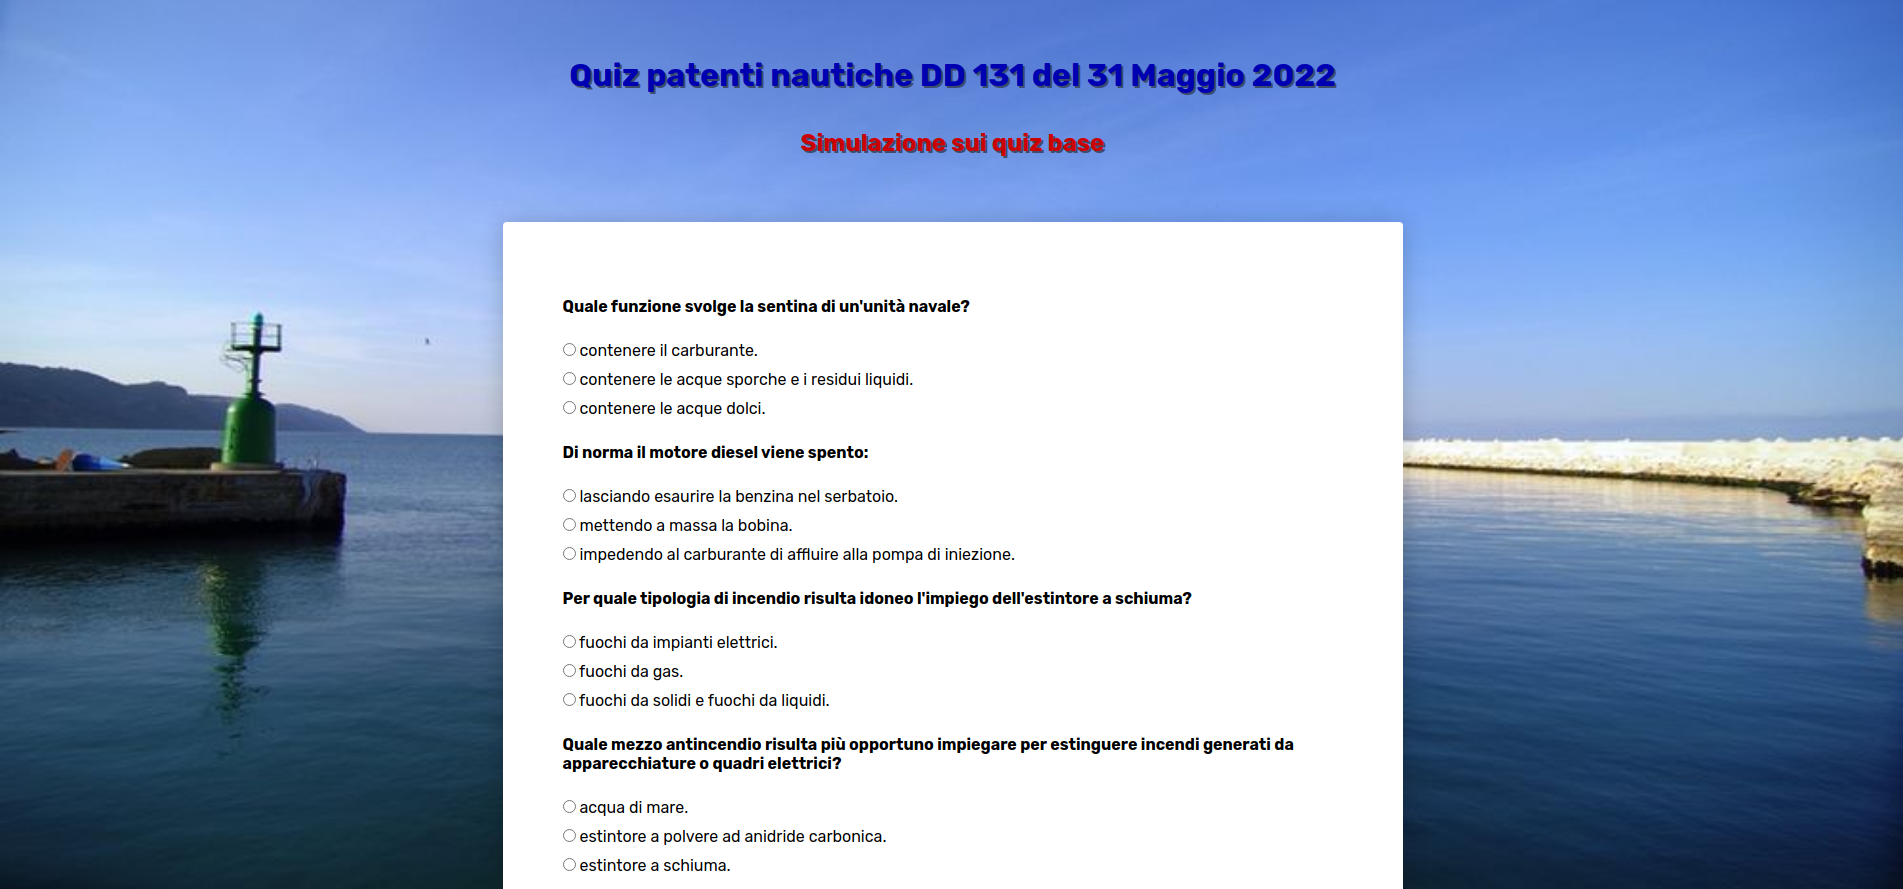
\includegraphics[scale=0.22]{Sites-images/28-Simulazione_quiz_base1.png}
		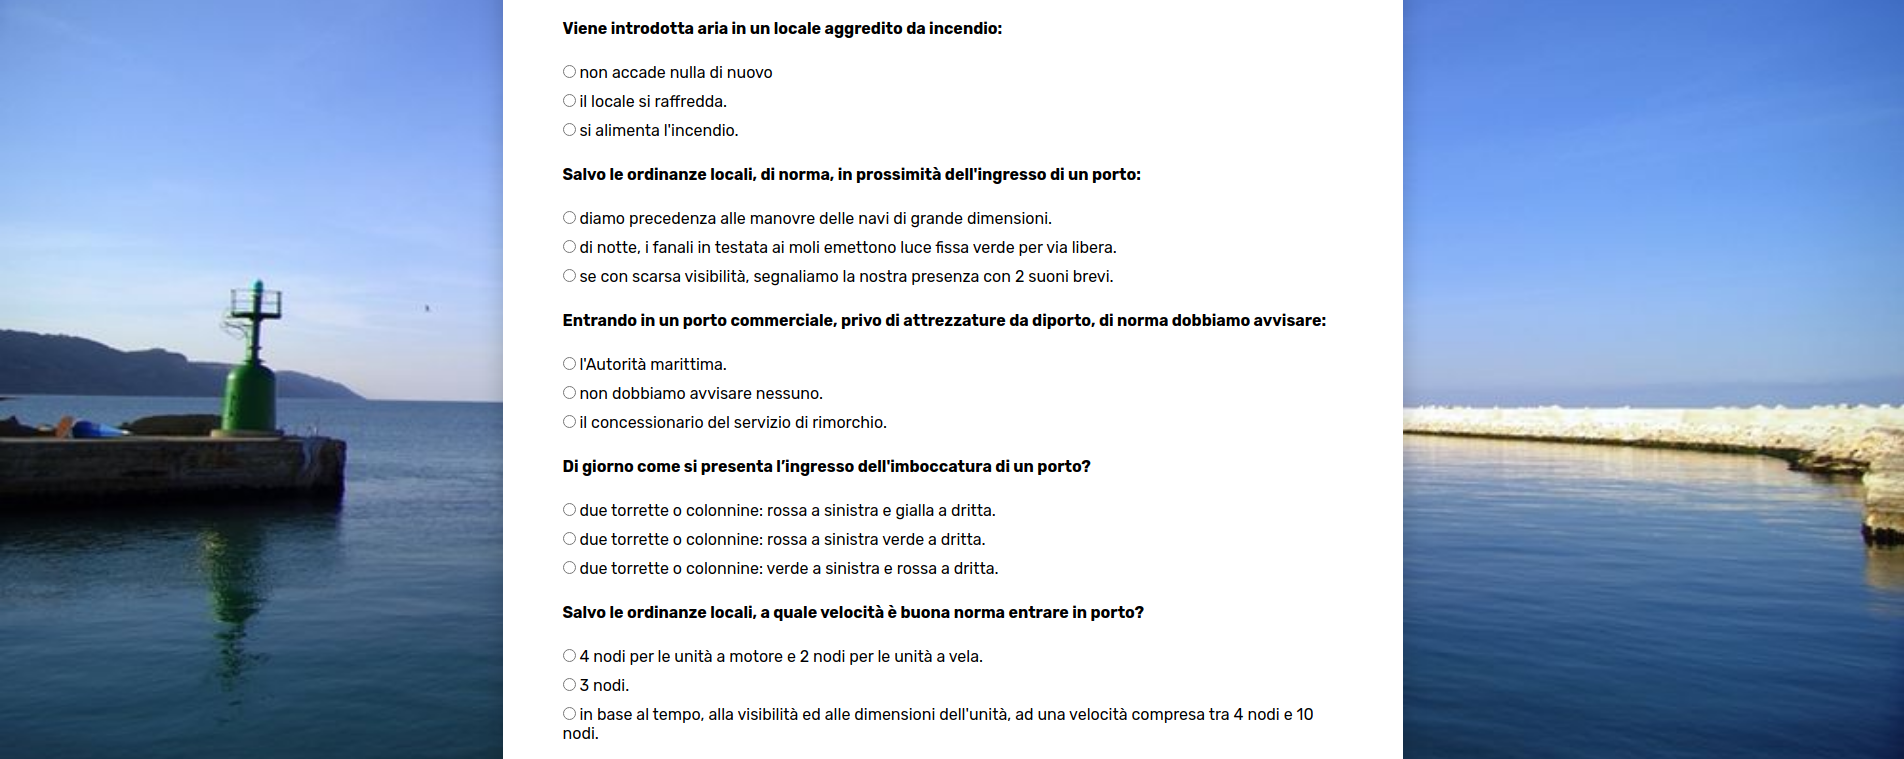
\includegraphics[scale=0.22]{Sites-images/29-Simulazione_quiz_base2.png}
		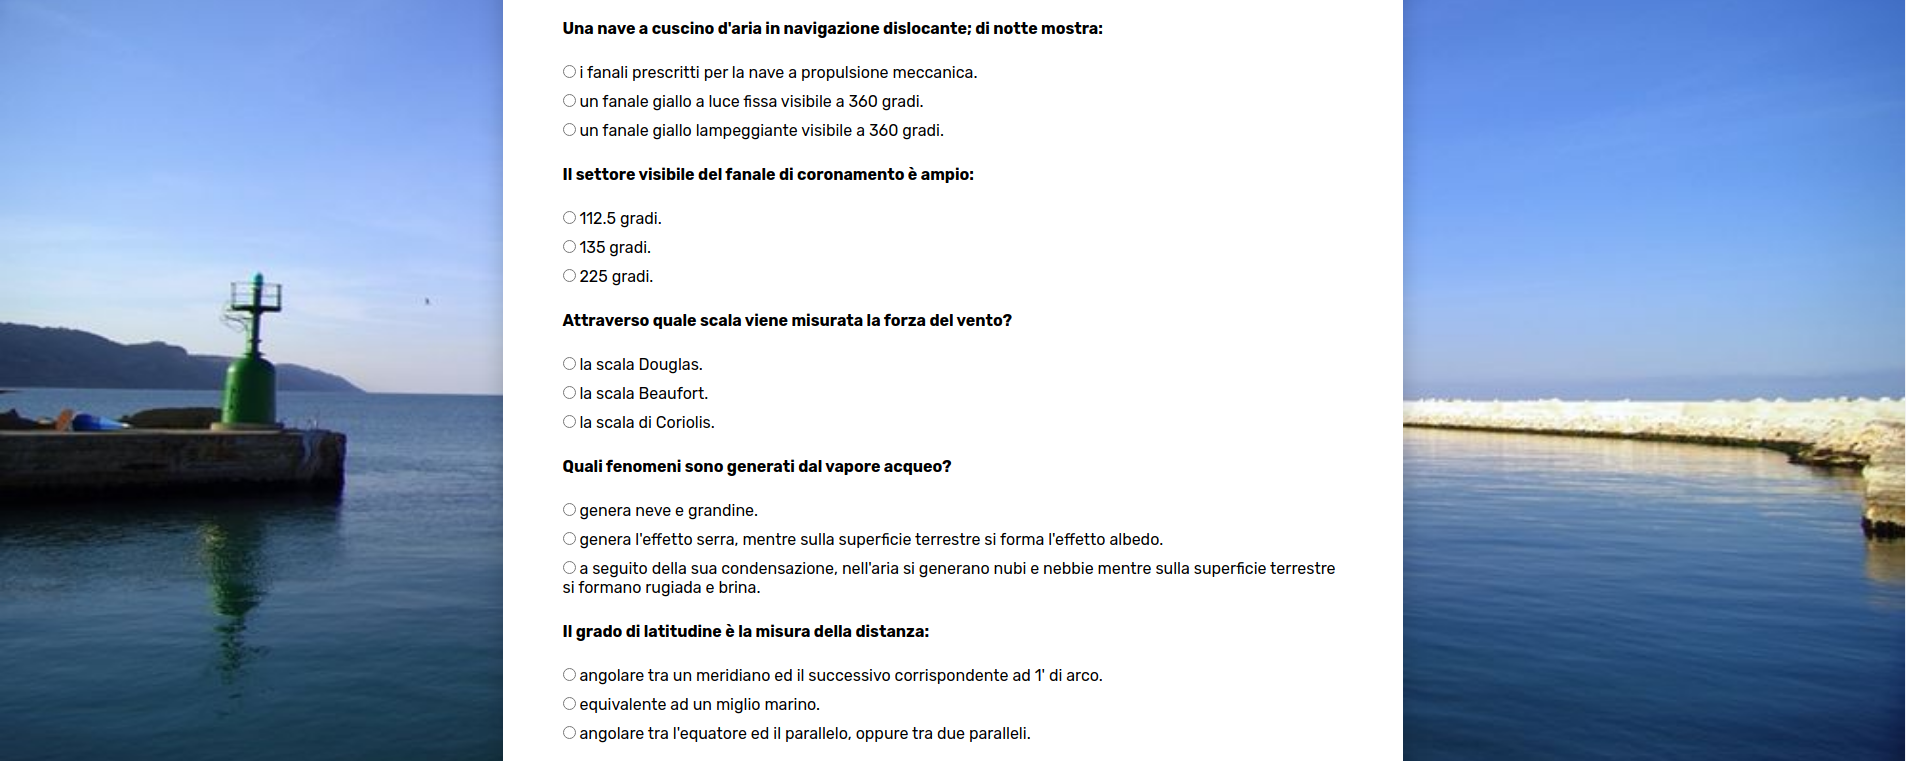
\includegraphics[scale=0.22]{Sites-images/30-Simulazione_quiz_base3.png}
		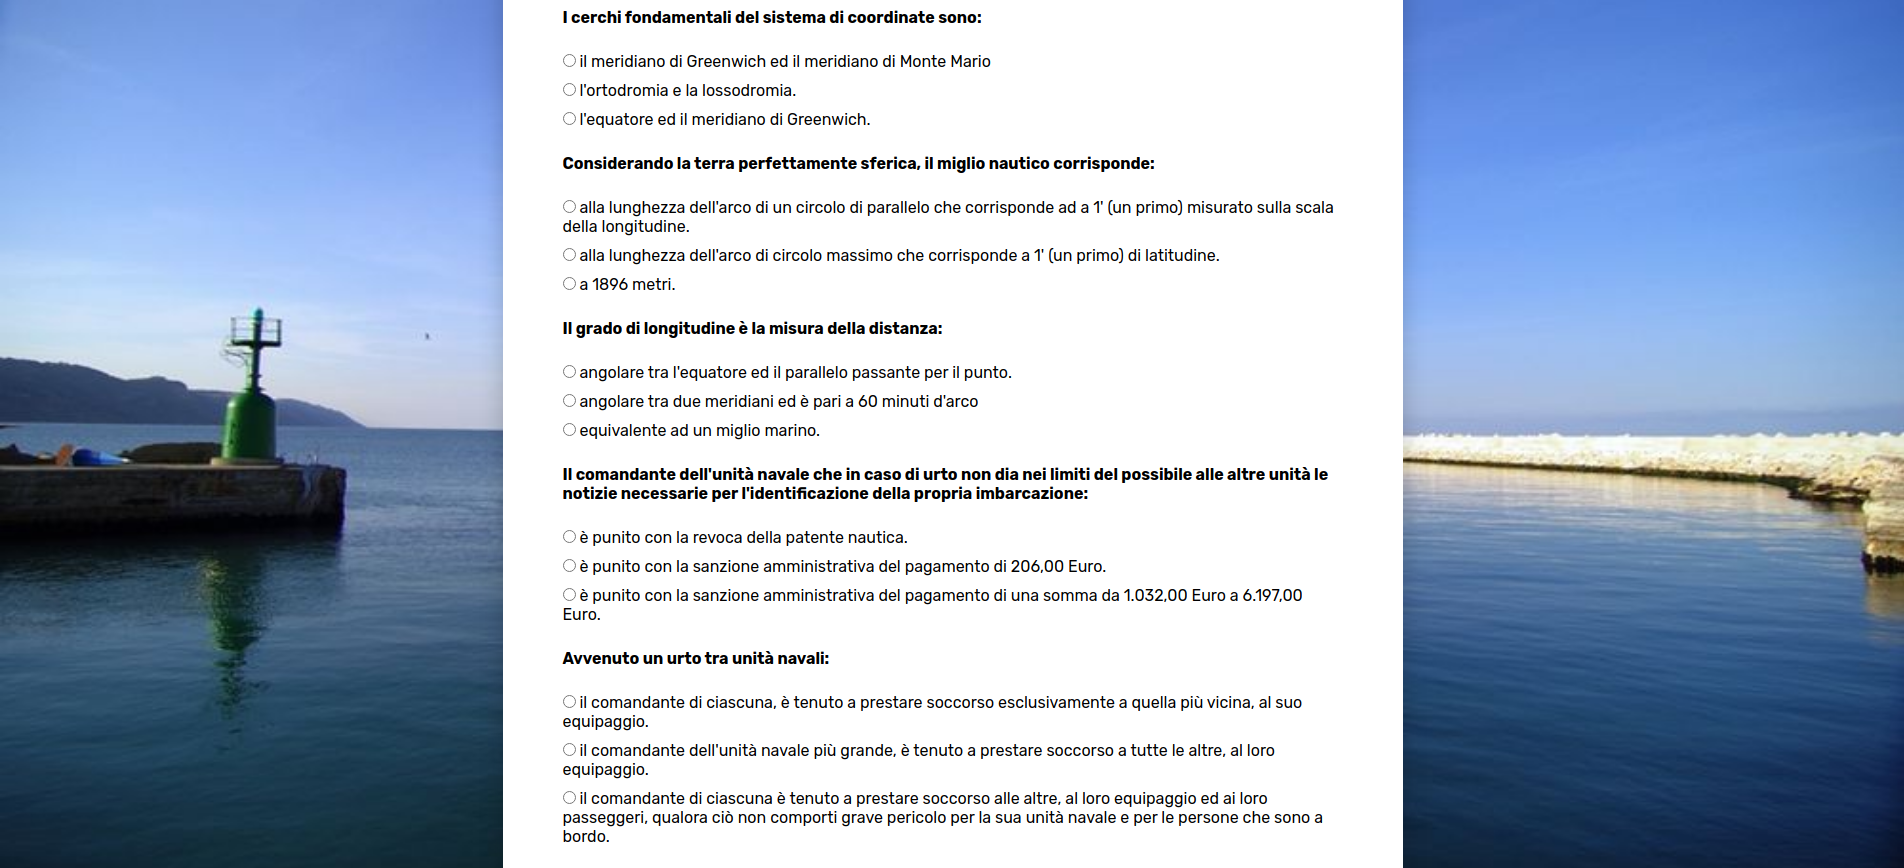
\includegraphics[scale=0.22]{Sites-images/31-Simulazione_quiz_base4.png}
		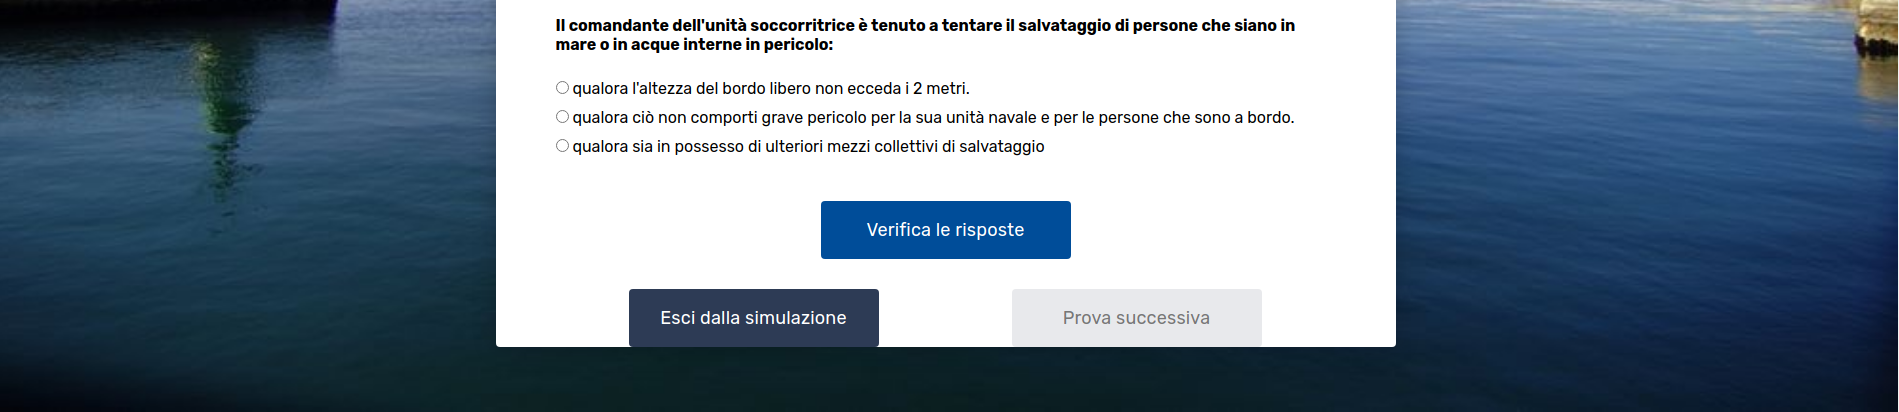
\includegraphics[scale=0.22]{Sites-images/32-Simulazione_quiz_base5.png}
		\caption{Pagina di simulazione dei quiz base.}
		(Ricomposta)
	\end{center}
\end{figure}
\end{minipage}

\begin{minipage}{\textwidth}
\begin{figure}[H]
	\begin{center}
		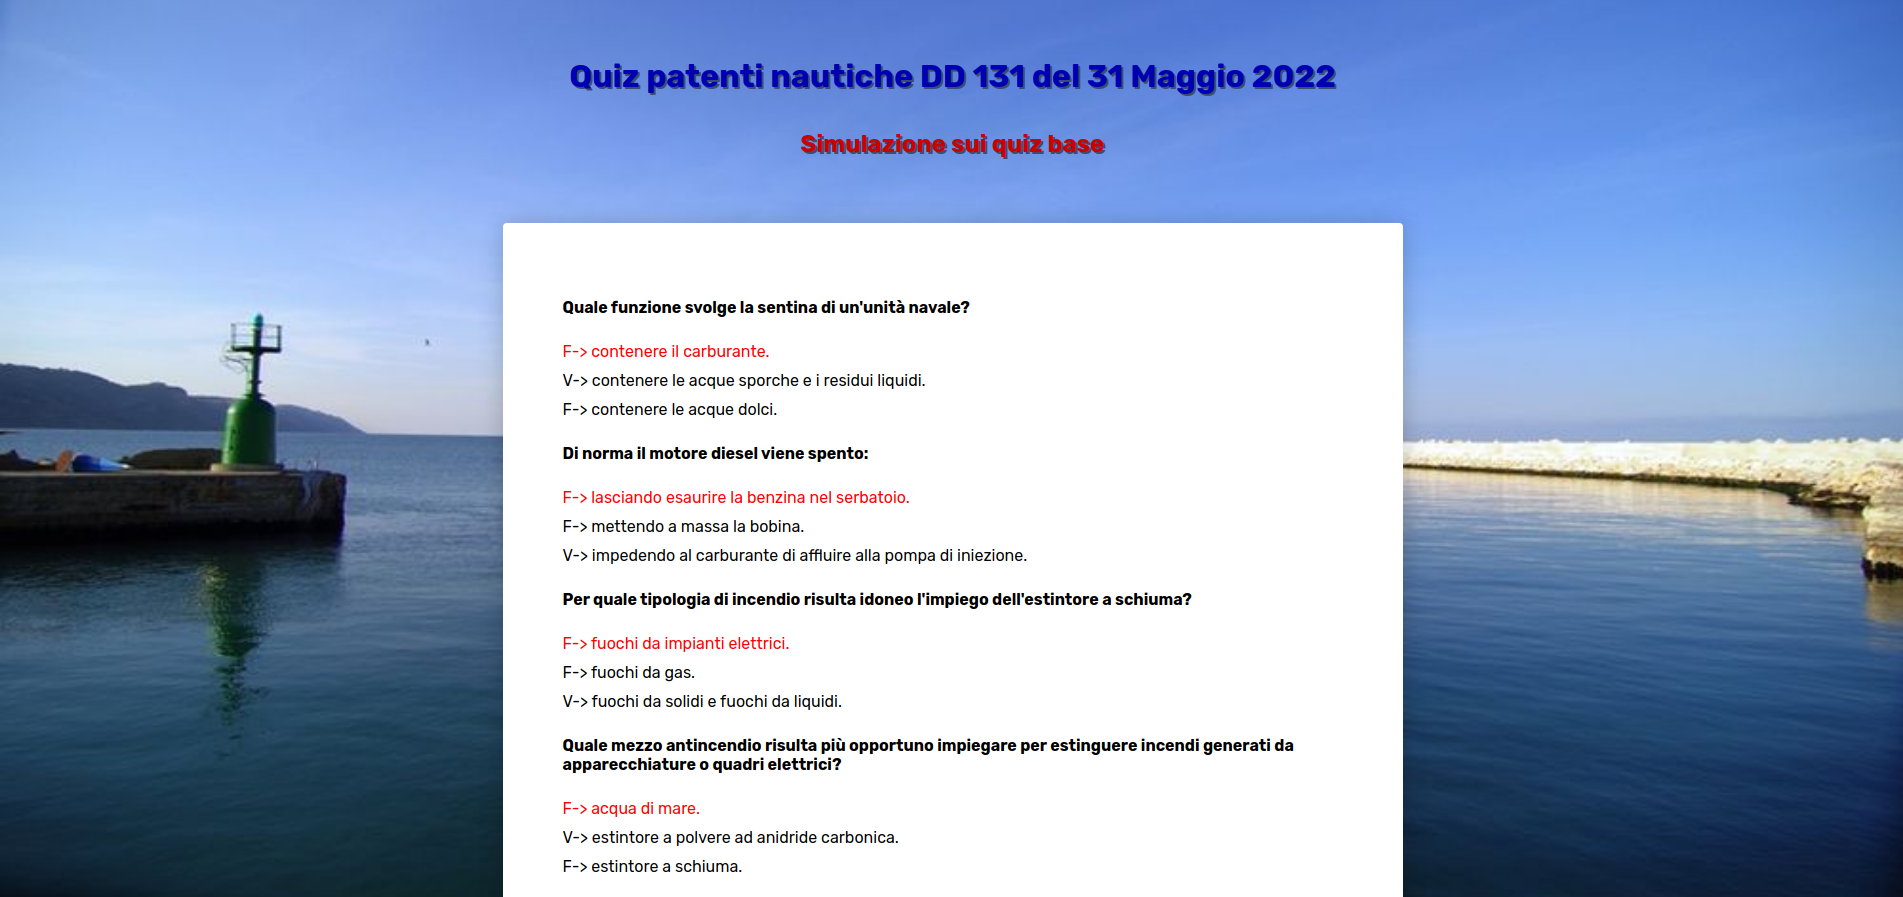
\includegraphics[scale=0.22]{Sites-images/33-Simulazione_quiz_base-risposte1.png}
		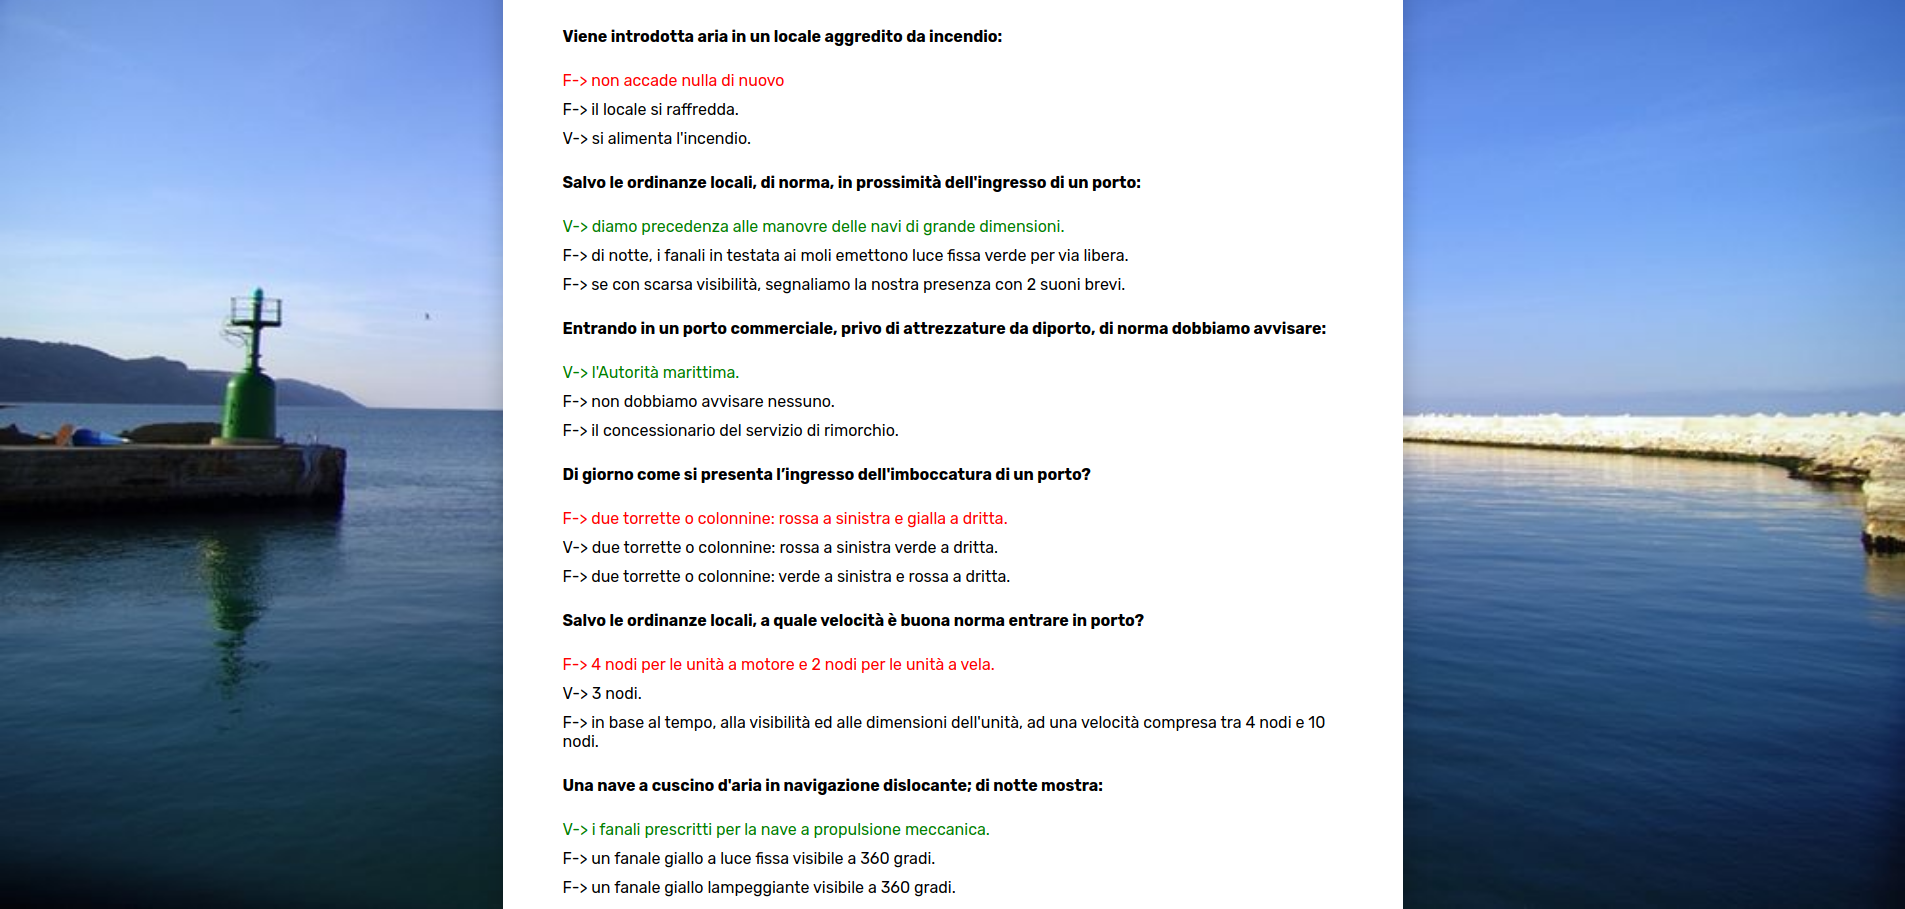
\includegraphics[scale=0.22]{Sites-images/34-Simulazione_quiz_base-risposte2.png}
		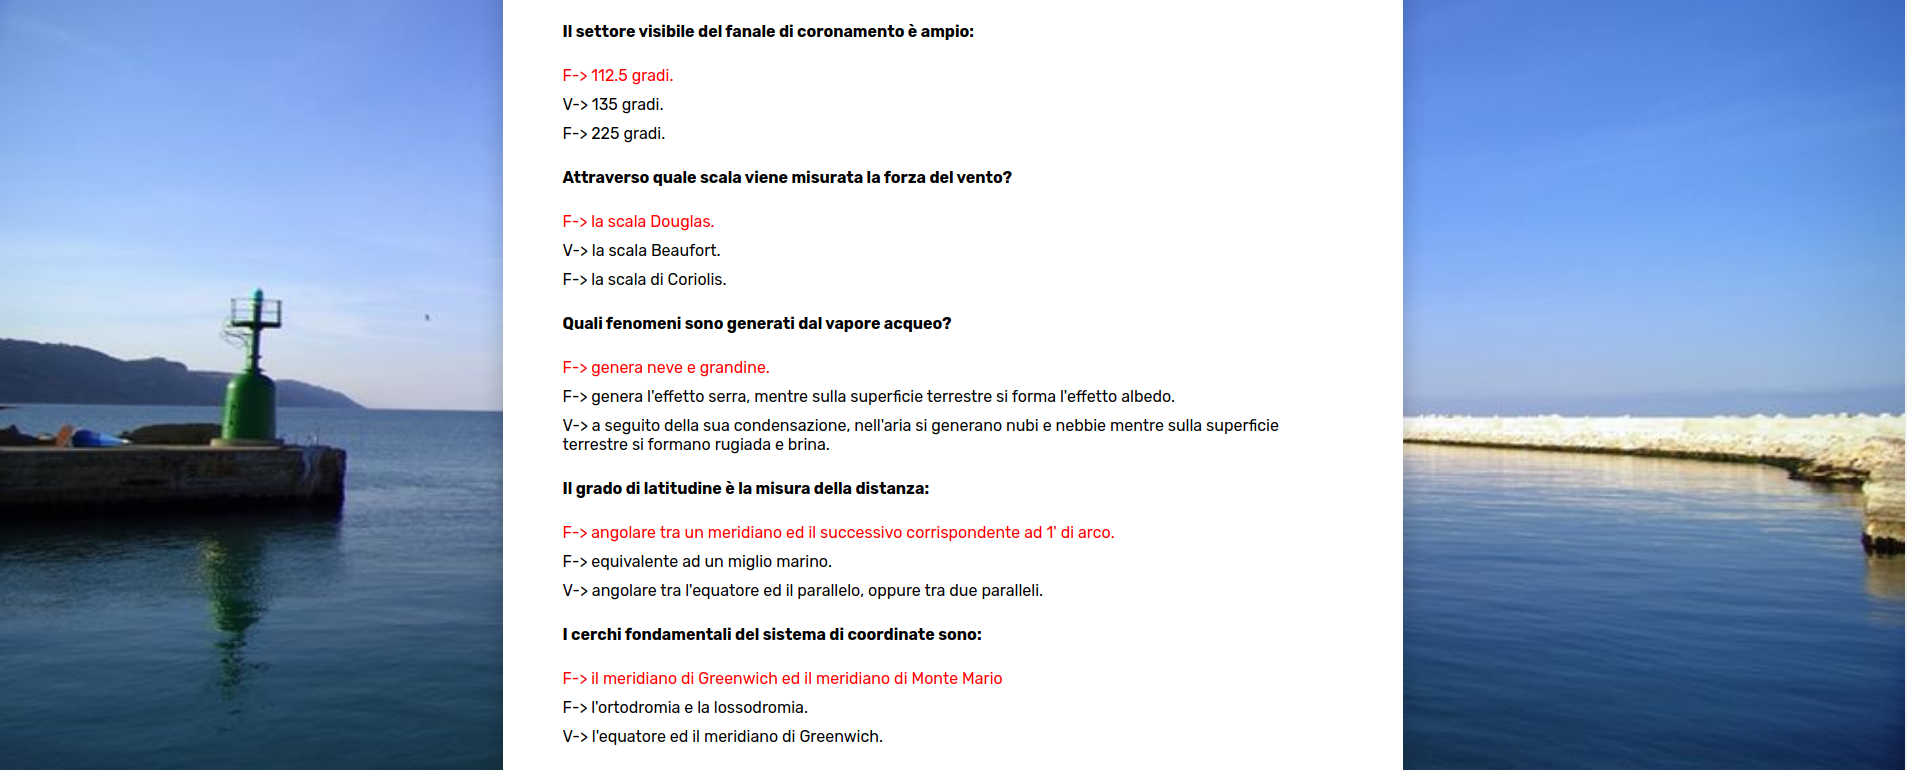
\includegraphics[scale=0.22]{Sites-images/35-Simulazione_quiz_base-risposte3.png}
		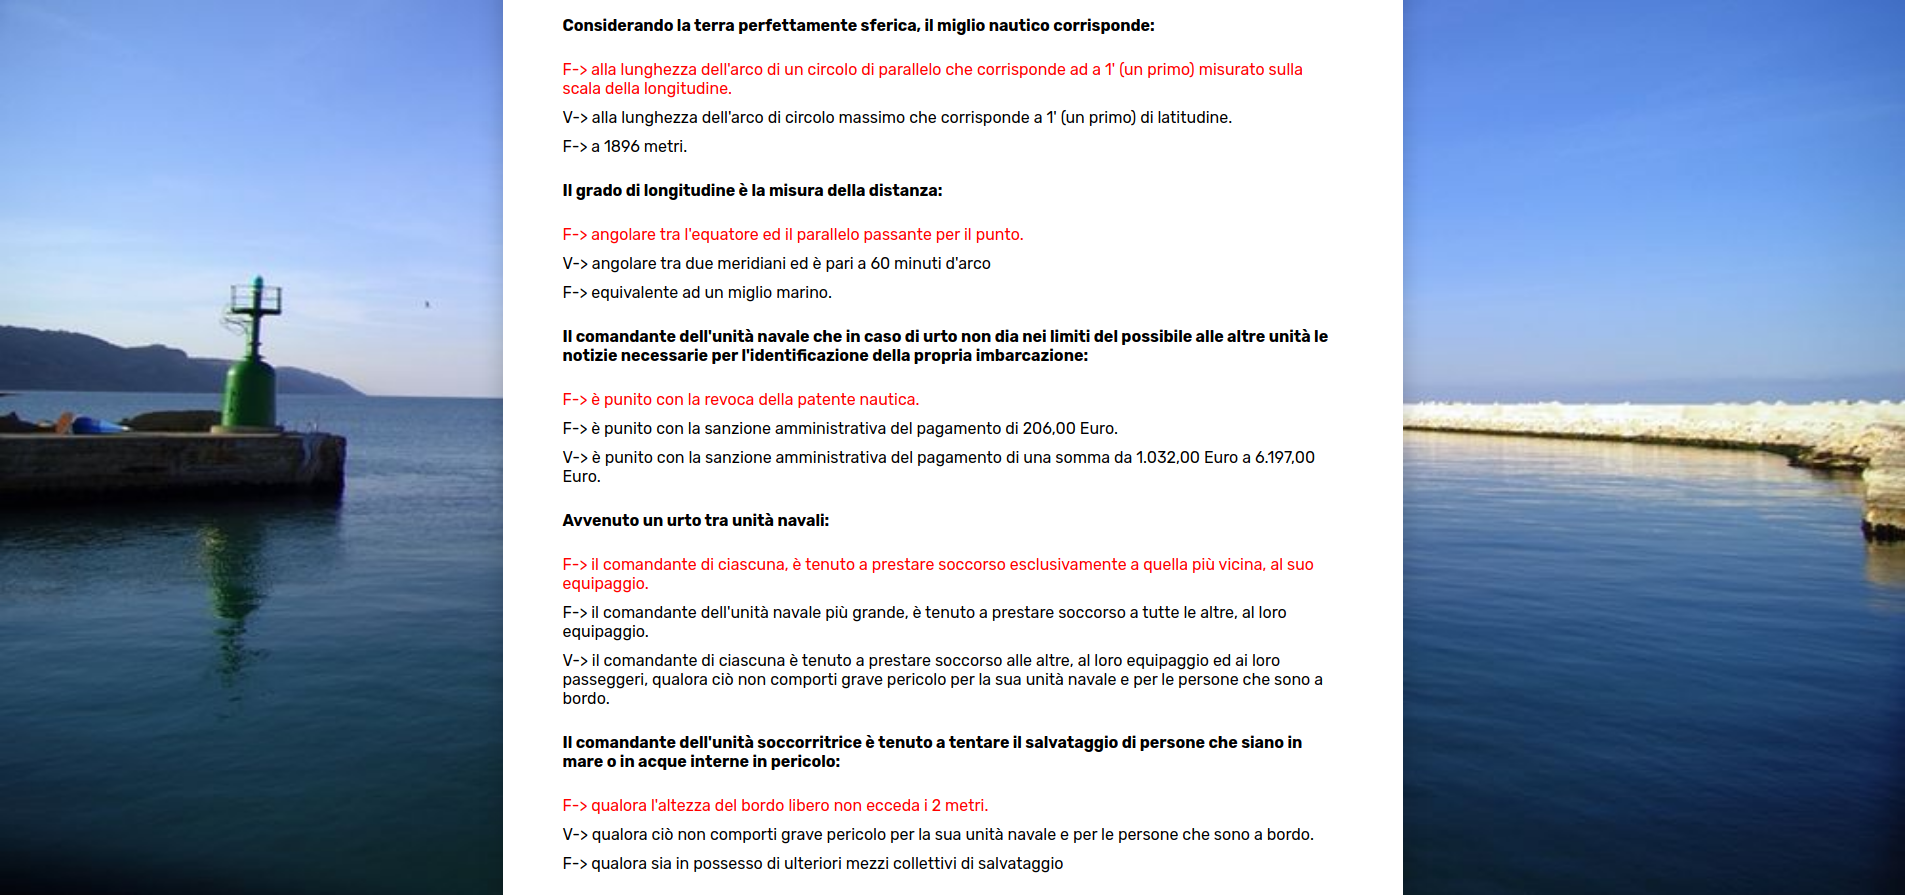
\includegraphics[scale=0.22]{Sites-images/36-Simulazione_quiz_base-risposte4.png}
		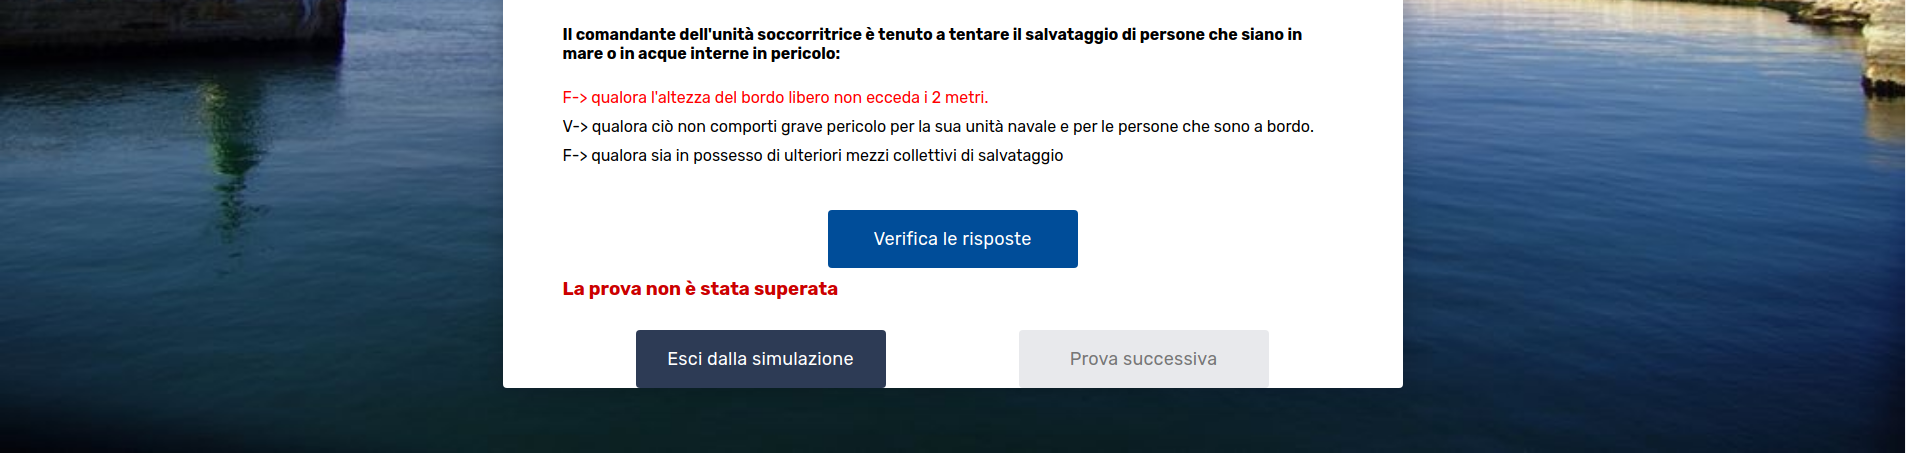
\includegraphics[scale=0.22]{Sites-images/37-Simulazione_quiz_base-risposte5.png}
		\caption{Pagina di simulazione dei quiz base con soluzioni.}
		(Ricomposta)
	\end{center}
\end{figure}
\end{minipage}

\textcolor{black}{Osservata la simulazione si analizza ora la parte di esercitazione associata alla simulazione.}\\

\paragraph{\textcolor{black}{Quiz base (esercitazione)}}\leavevmode\\
\raggedright
\textcolor{black}{L'unica novità rispetto al passato è il fatto che anche in questo esercizio si tiene il conto degli errori commessi. La problematica risiede sempre nella comunicazione tra "front-end" e "back-end", siccome è solo la parte del "javascript" che è in grado di verificare le risposte (la pagina mostra e corregge una domanda per volta). La soluzione (in linea con il passato) è stata quella di mettere in comunicazione questi due emisferi salvando dei parametri "nell'url", primo tra tutti il tipo di domande scelte come nel caso della esercitazione sulla prova di carteggio, date le problematica nel far funzionare "AJAX".\\
Qui di seguito è riportato il codice in "php".}\\

\begin{lstlisting}[language=php]
/*---------- CATCH URL VARIABLES ----------*/
$Array = $urlUtility->getInfoFromUrl($_SERVER['REQUEST_URI']);

//---------- CATCH SCORE
if($Array['score'] !== null){
	$_SESSION['score'] = $Array['score'];
}

//---------- CATCH LAST QUESTIONS VARIABLES
if($Array['index'] !== null && $Array['answer'] !== null){
	
	if($_SESSION['answeredQuestions'][$Array['index']] == null){
		$_SESSION['answeredQuestions'][$Array['index']] = $Array['answer']; 
	} 
}

//---------- CATCH TOPIC 
if($Array['topic'] !== null && $Array['topic'] !== $_SESSION['topic']){
	$_SESSION['topic'] = $Array['topic'];
	
	/*change temp array to determinate questions*/
	$query = $utilities->getMysql()->query("SELECT * FROM base_quiz WHERE (topic = '{$Array['topic']}')");
	$tempArray = $query->fetch_all(MYSQLI_ASSOC);
	/*format variables for question preparation part*/
	$_SESSION['maxQuestions']         = null;
	//get number of extracted questions
	$_SESSION['questions']            = $tempArray;
	$_SESSION['numbers']              = 0;
	$_SESSION['score']                = 0;
	$_SESSION['answeredQuestions']    = null;
}
\end{lstlisting}

\textcolor{black}{Nel codice appena mostrato vi è una funzionalità (implementata a livello di "php" con il "catch" dell'ultima risposta data, trasmessa dal "javascript") che permette di tenere in sessione le risposte date in precedenza in modo da poterle ricontrollare anche in un secondo momento. Il resto del codice in "php" non presenta differenze sostanziali rispetto a quanto è già stato mostrato  e anche il codice "html" è intuibile tenendo a mente quello scritto nel caso della simulazione.\\
Nel caso del "javascript" una cosa da evidenziare è l'inserimento dei parametri "nell'url" e anche come vengono gestire le riposte date in precedenza.}\\

\vspace*{1cm}

\begin{lstlisting}[language=java]
	
	/*--------- SECTION WHERE VERIFY IF THE QUESTION WAS ANSWERED ----------*/
	//useful variables
	var questionIndex = <?php if($id !== null){echo $id;}else{echo "-1";}?>;
	var answerGiven = null;
	
	//verified the past answer
	if(Boolean(<?php if($_SESSION['answeredQuestions'][$id] !== null){echo true;}else{echo false;}?>)){
		
		// to not permit other review
		corrected = true;
		
		switch(<?php if($_SESSION['answeredQuestions'][$id] !== null) {echo $_SESSION['answeredQuestions'][$id];}else{echo "-1";} ?>){
			
			case <?php echo ANSWER1; ?>:
			
			answerRadios.style.display = "none";
			answer1.style.display      = "block";
			answer2_null.style.display = "block";
			answer3_null.style.display = "block";
			break;
			
			case <?php echo ANSWER2; ?>:
			
			answerRadios.style.display = "none";
			answer1_null.style.display = "block";
			answer2.style.display      = "block";
			answer3_null.style.display = "block";
			break;
			
			case <?php echo ANSWER3; ?>:
			
			answerRadios.style.display = "none";
			answer1_null.style.display = "block";
			answer2_null.style.display = "block";
			answer3.style.display      = "block";
			break;
			
		}
		
	}
	
	// set argument topic to url
	function setArgument(topic){
		var URL = window.location.href;
		var data ={'topic': topic};
		var parameters = new URLSearchParams(data);
		window.location.href = URL.split('?')[0]+"?"+parameters;
	}

	//set the new score to url
	function setScore(score){
		var URL = window.location.href;
		var data ={'score': score};
		var parameters = new URLSearchParams(data);
		window.history.pushState(null, document.title, (URL.split('?')[0]+"?"+parameters))
	}

	//set the answer given to php session by url
	function setAnswerGiven(index, answer){
		var URL = window.location.href;
	
		var data1 ={'index': index};
		var data2 ={'answer': answer};
		var parameters1 = new URLSearchParams(data1);
		var parameters2 = new URLSearchParams(data2);
		window.history.pushState(null, document.title, (URL+"&"+parameters1+"&"+parameters2));
	}
\end{lstlisting}\leavevmode

%\newgeometry{bottom=1cm}

\begin{minipage}{\textwidth}
%\vspace*{-2cm}
	\textcolor{black}{Purtroppo anche in questa situazione non potendo utilizzare "AJAX" si sono dovuti trovare dei "workaround" per permettere comunque l'implementazione di queste funzionalità ritenute importanti.\\
	Nel caso in cui nella pagina venga caricata una domanda alla quale si è già risposto, viene eseguita in automatico la correzione, prendendo come valore per la risposta data in precedenza.\\
	Altra cosa qui mostrata è come sono stati salvati tutti i paramatri "nell'url" in modo da poter essere poi ripresi dalla parte in "php".}\\
\end{minipage}\leavevmode\newpage

\begin{minipage}{\textwidth}
\begin{figure}[H]
	\begin{center}
		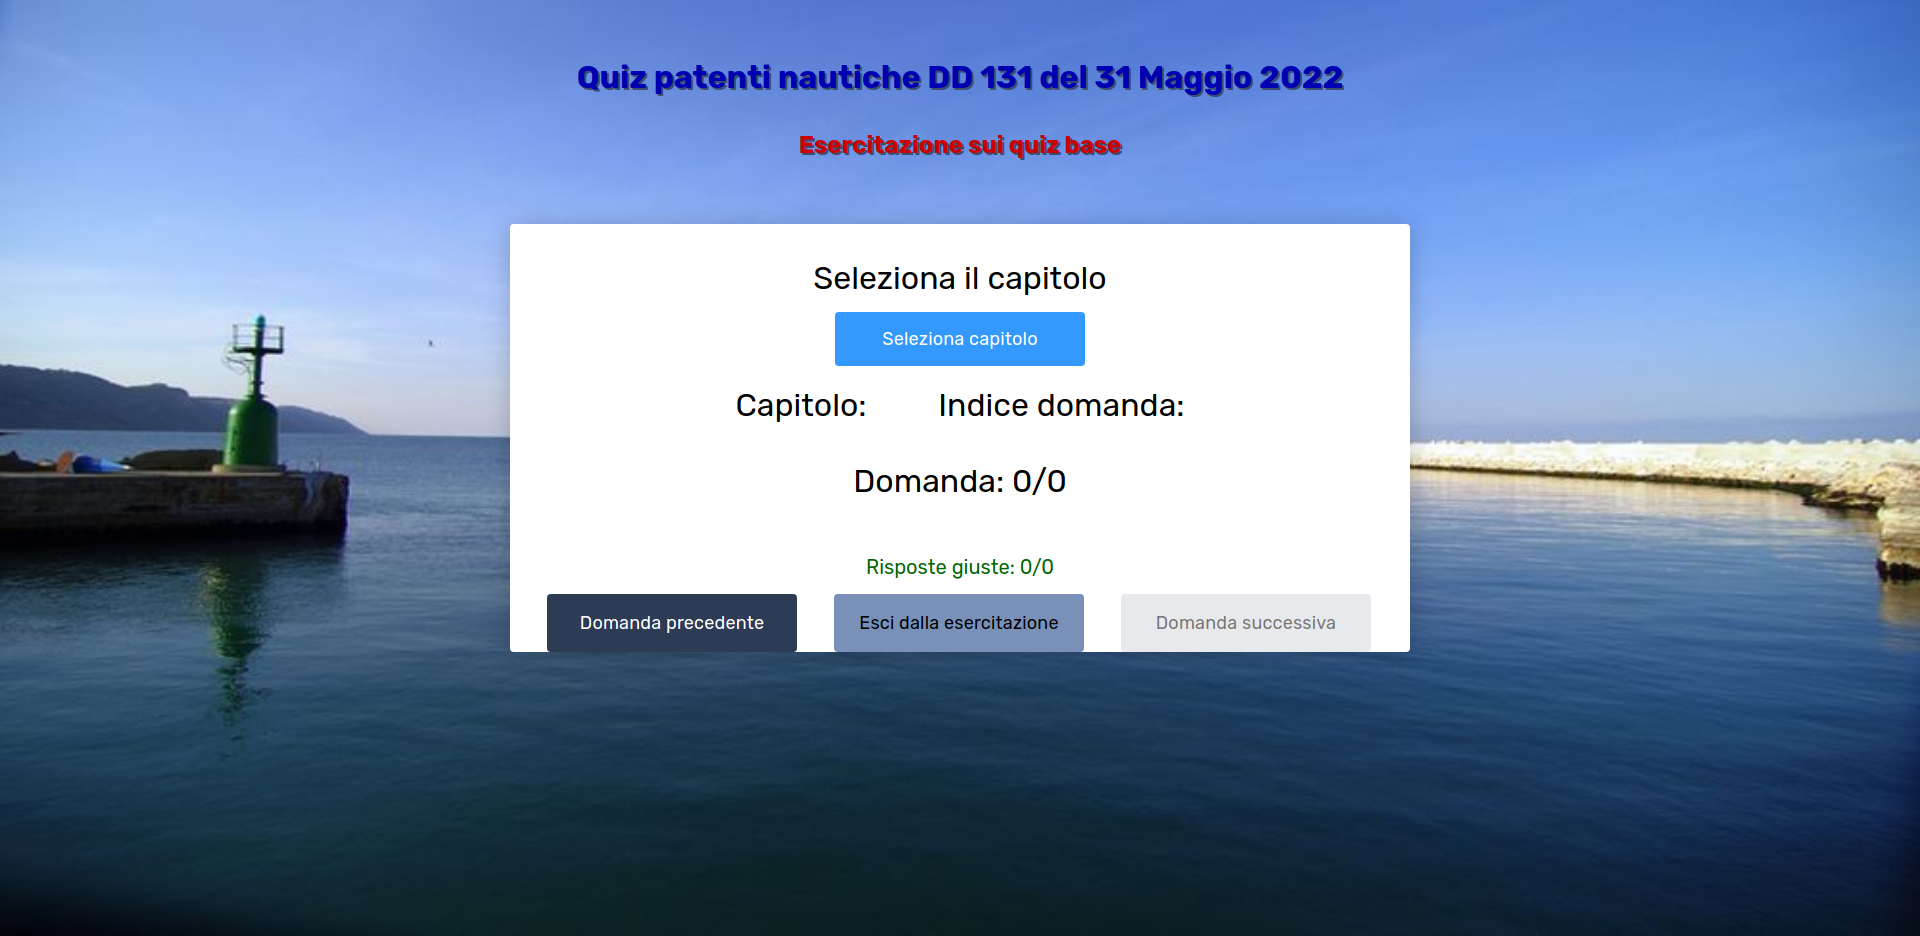
\includegraphics[scale=0.25]{Sites-images/38-Quiz_Base.png}
		\caption{Pagina dei quiz base.}
	\end{center}
\end{figure}


\begin{figure}[H]
	\begin{center}
		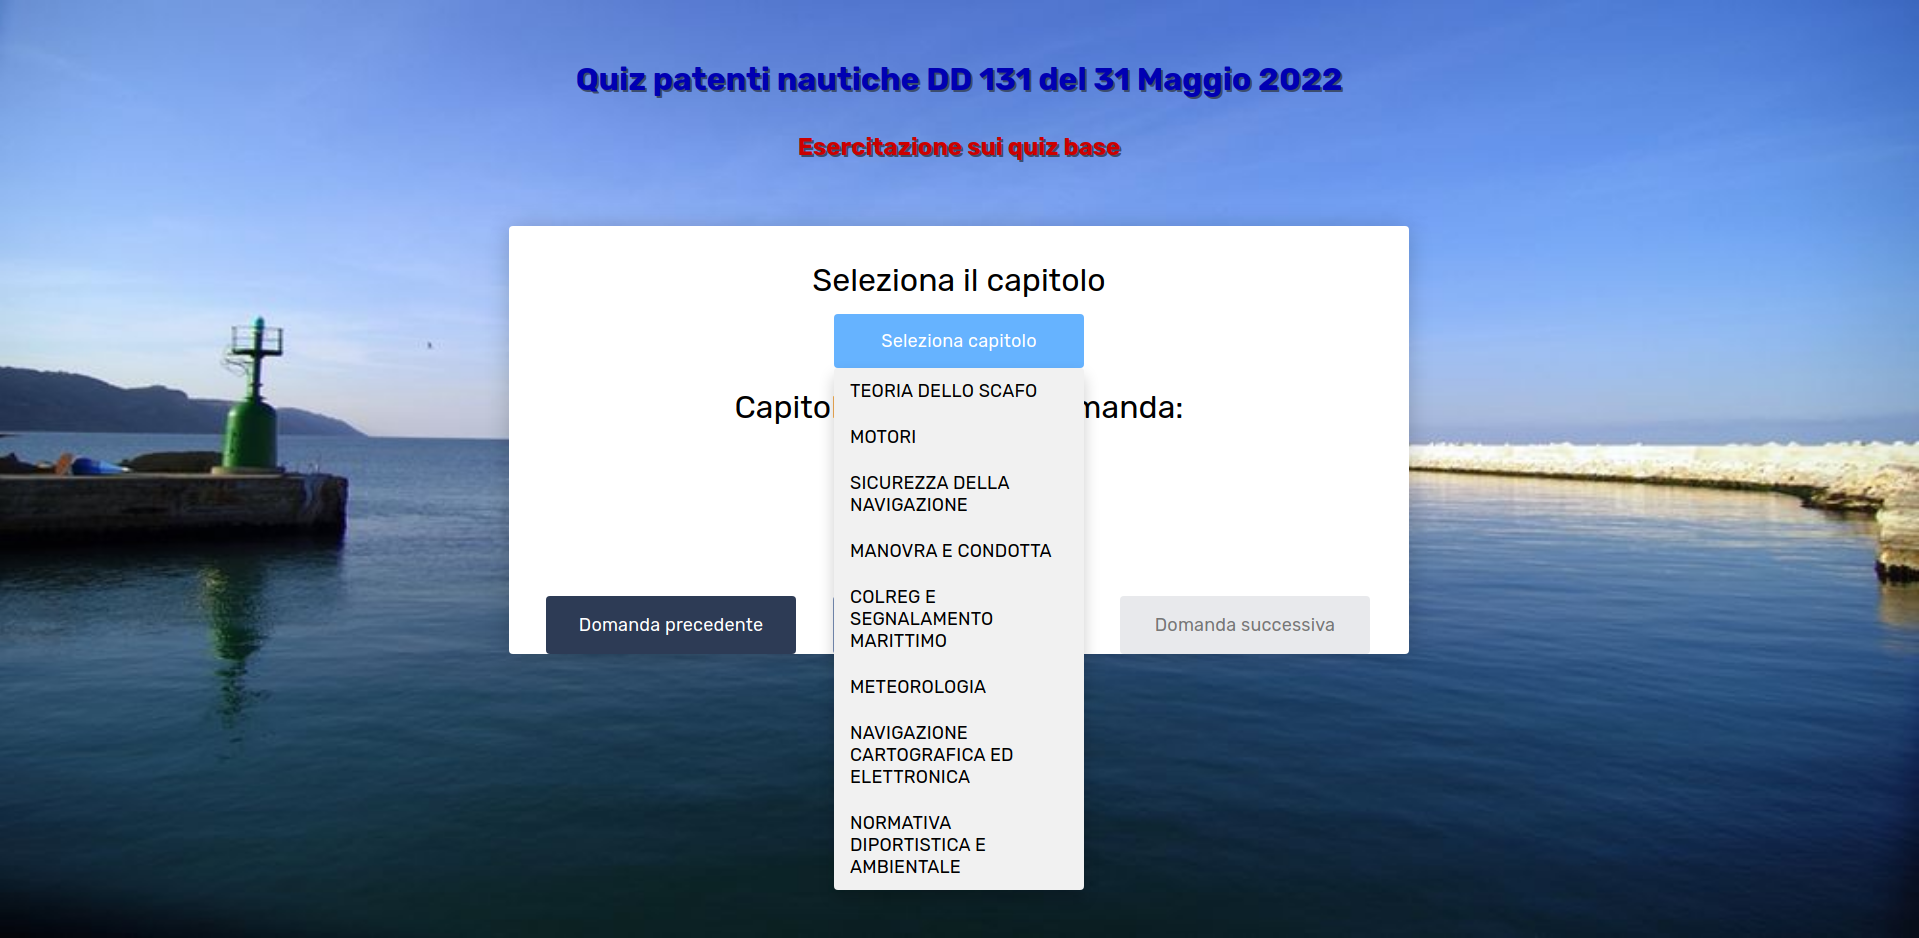
\includegraphics[scale=0.25]{Sites-images/39-Quiz_Base_selezione.png}
		\caption{Pagina dei quiz base con selezione.}
	\end{center}
\end{figure}

\begin{figure}[H]
	\begin{center}
		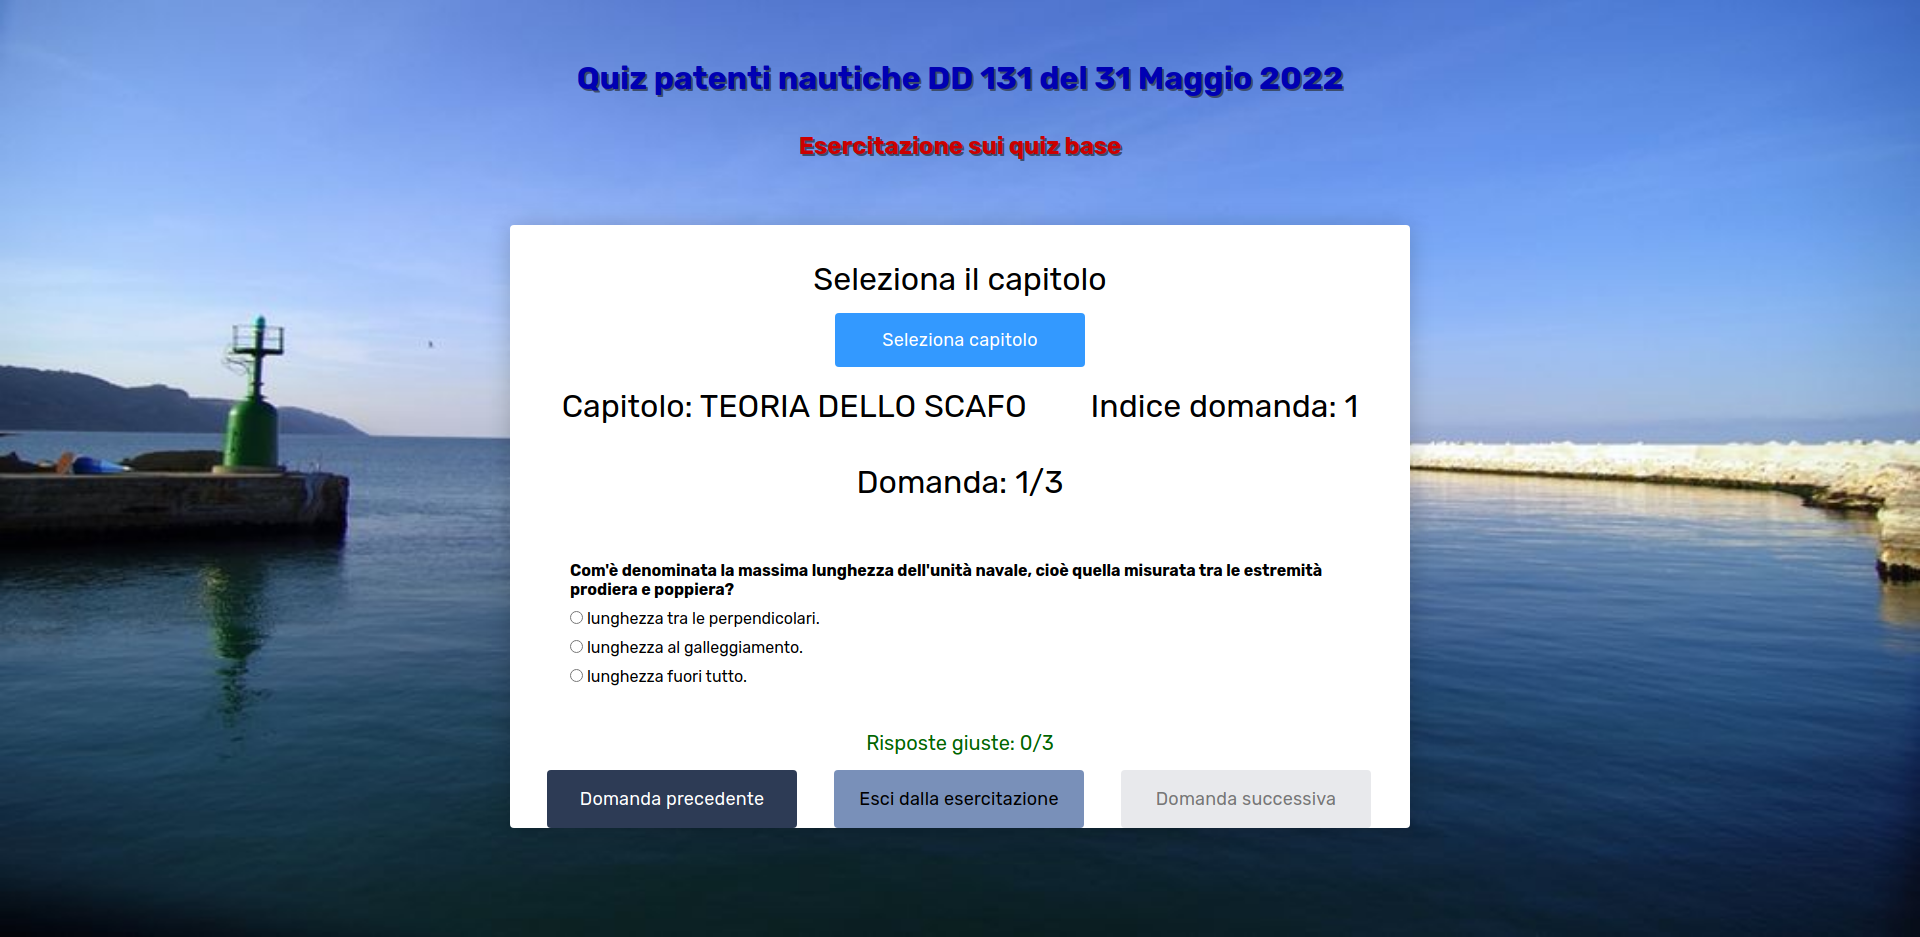
\includegraphics[scale=0.25]{Sites-images/40-Quiz_Base_Domanda.png}
		\caption{Pagina dei quiz base con domanda.}
	\end{center}
\end{figure}
\end{minipage}

\begin{minipage}{\textwidth}
\begin{figure}[H]
	\begin{center}
		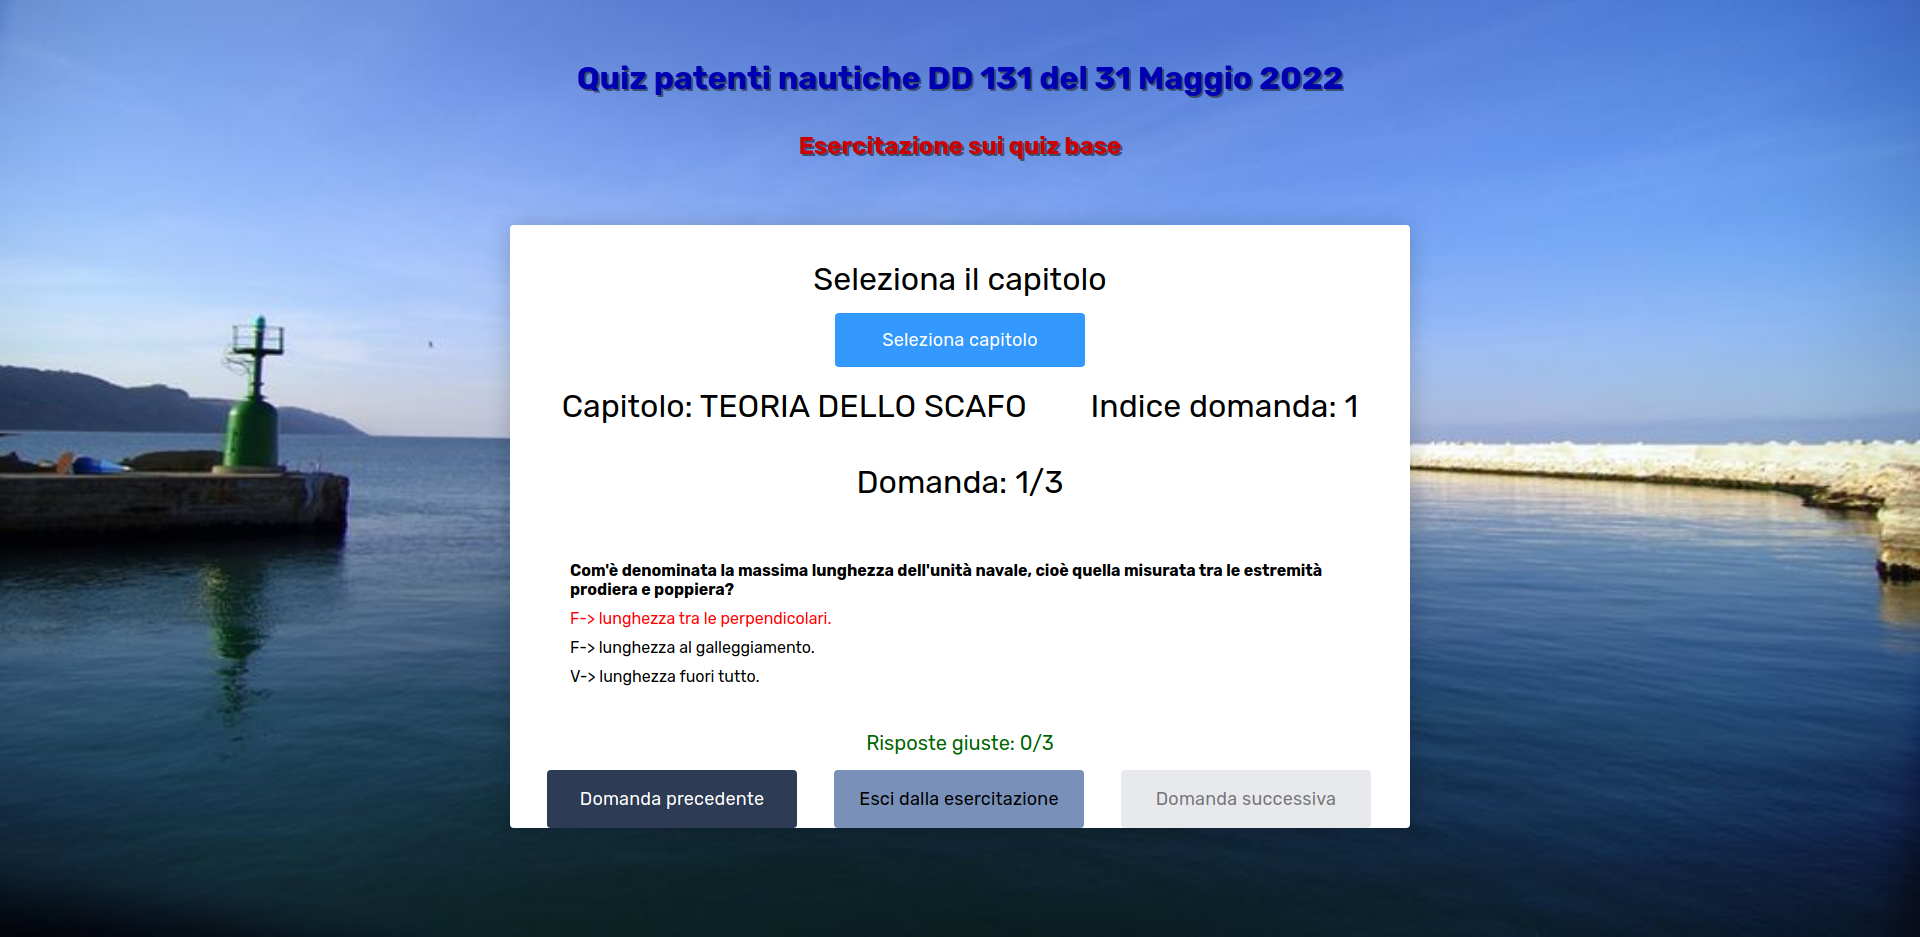
\includegraphics[scale=0.25]{Sites-images/41-Quiz_Base_Soluzione.png}
		\caption{Pagina dei quiz base con soluzione.}
	\end{center}
\end{figure}
\end{minipage}

\textcolor{black}{L'ultima parte del sito implementata, ovvero la simulazione e l'esercitazione dei quiz della vela non viene riportata, in quanto sulla base di quello che è stato mostrato finora sarebbe una ripetizione di logiche e di codice già visto.} 

		%\ringraziamenti
		%\textbf{Non so a chi ringraziare}

	\end{document}
